\documentclass[12pt,oneside]{book}

\usepackage[dvips,letterpaper,margin=0.75in,bottom=0.75in]{geometry}
\usepackage{cite}
\usepackage{slashed}
\usepackage{graphicx}
\usepackage{amsmath}
\usepackage{enumitem}
\usepackage{amsthm}
\usepackage{braket}
\theoremstyle{definition}

\usepackage[american,fulldiode]{circuitikz}
\tikzset{component/.style={draw,thick,circle,fill=white,minimum size =0.75cm,inner sep=0pt}}
\newtheorem{measurement}{Logbook Entry}[chapter]
\newtheorem{plot}{Jupyter Notebook}[chapter]

\begin{document}
\ctikzset{bipoles/thickness=1}
\ctikzset{bipoles/length=.6cm}

\title{Physics 80 Lab Manual}
\author{Michael Mulhearn, Emilija Pantic}
\maketitle

\tableofcontents

\chapter{Introduction to Scientific Python}

\section{Introduction}

This lab will highlight key Scientific Python features starting from
Python fundamentals.

\section{Starting a Jupyter notebook}

This course will make extensive use of the Jupyter Notebook interface
to Scientific Python, which is well suited to academic work (including
independent research) because it combines code with output in
digestable chunks.  Even when the end product is a polished peice of
software, much of the development occurs in the sort of interactive
sessions that Jupyter Notebooks provide.  

\begin{figure}[htbp]
\begin{center}
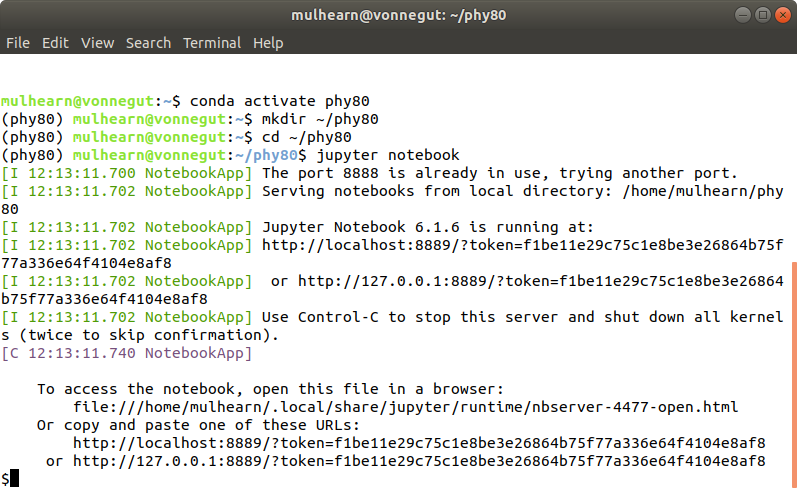
\includegraphics[width=0.65\textwidth]{figs/labs/python/jupyter_startup.png} 
\caption{Example starting Jupyter Notebook from the Linux command line.  In Windows, you will need to open the Anaconda Prompt instead of a terminal.}
\label{fig:jupyterstartup}
\end{center}
\end{figure}

\begin{figure}[htbp]
\begin{center}
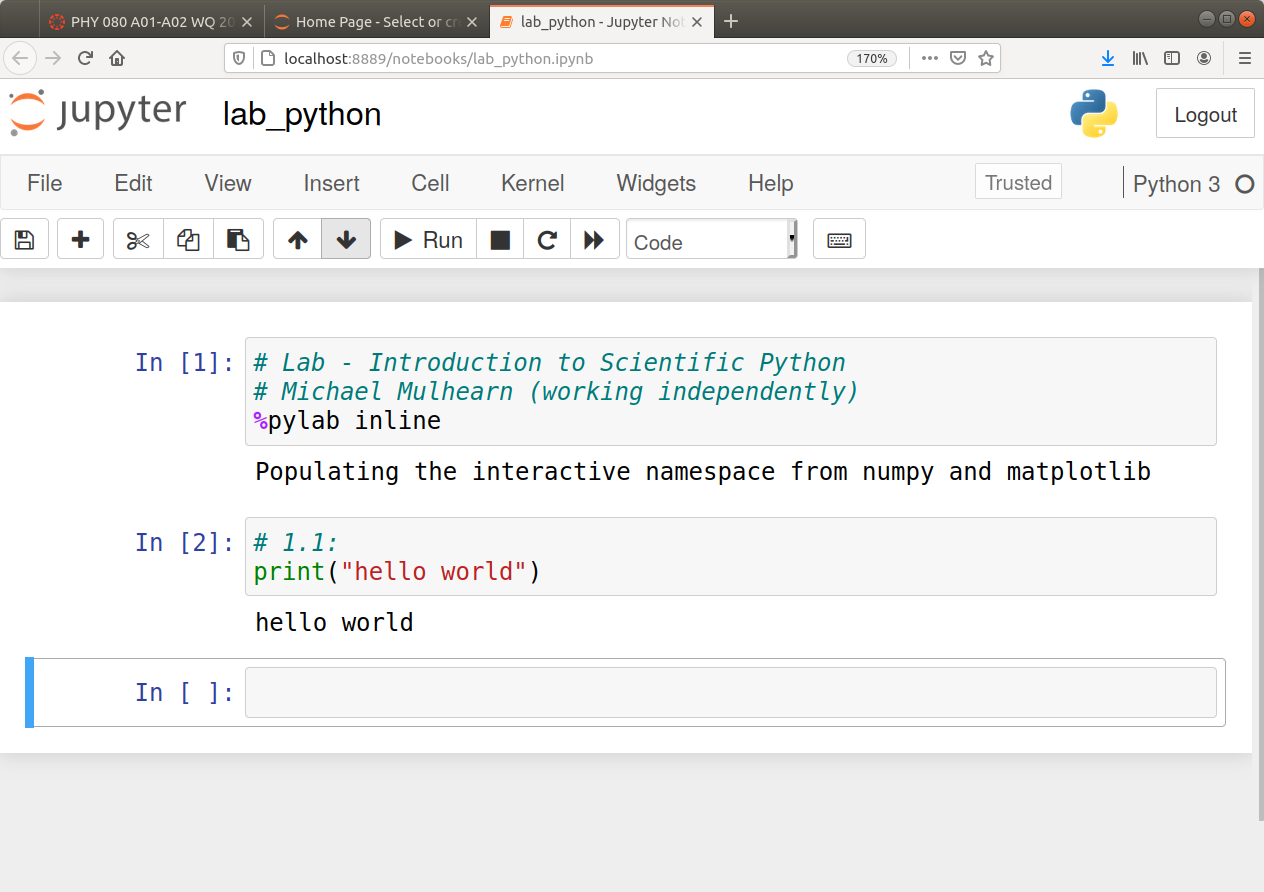
\includegraphics[width=0.65\textwidth]{figs/labs/python/jupyter_window.png} 
\caption{The Hello World example Jupyter Notebook.}
\label{fig:jupyterwindow}
\end{center}
\end{figure}

\begin{figure}[htbp]
\begin{center}
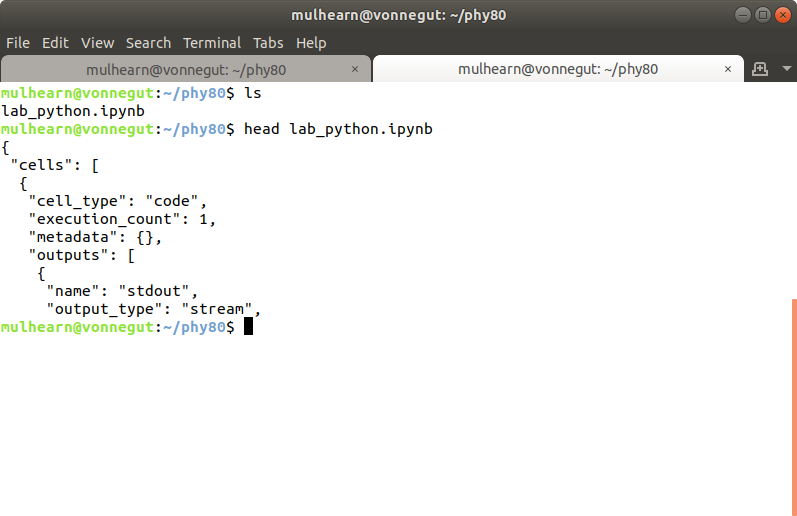
\includegraphics[width=0.65\textwidth]{figs/labs/python/jupyter_saved.png} 
\caption{Example showing the saved Jupyter notebook.  Notice that notebook file (ipynb) is not human readable on its own: it requires the Jupyter software to render it in a human readable form.}
\label{fig:jupytersaved}
\end{center}
\end{figure}

After following the software installation instructions on the course
website, activate the Physics 80 environment with:
\begin{verbatim}
$ conda activate phy80
\end{verbatim}
Then, navigate to a working directory for this session, and start the notebook with:
\begin{verbatim}
$ jupyter notebook
\end{verbatim}
This should start the Jupyter Notebook server and open a client in your web browser.
An example starting a Jupyter Notebook from Linux is shown in Fig.~\ref{fig:jupyterstartup}.

You should create one Jupyter Notebook per lab assignment, by choosing
the New (Python 3) option in your client.  Change the name of your
notebook to something that clearly identifies the lab.  Start each lab
with comments (starting with ``\#'' symbol) indicating the title of
the lab, then your name followed by your lab partners.  See the first
cell of Fig.~\ref{fig:jupyterwindow} for an example.  This first cell
is also a good place to issue the ipython ``magic function'':
\begin{verbatim}
%pylab inline
\end{verbatim}
which will setup the notebook for inline plots and load the numpy and matplotlib libraries for you.

Each assignment will consist of a number of steps, clearly numbered like this one, you first step:

\begin{plot}
Print ``hello world'' using the python print command.
\end{plot}
\noindent
To keep your notebook clear, label cells (such as this one) with a
comment for the assignment step number, as in the second cell of
Fig.~\ref{fig:jupyterwindow}.  You only need to label one cell if
the assignment is fullfilled across several cells.

Jupyter Notebook checkpoints your work automatically.  You should be
able to see your notebook saved in the working directory where you
started, as in Fig.~\ref{fig:jupytersaved}.  Notice that while the
notebook file is ASCII text, it is not a human readable format.  The
Jupyter software is needed to render the notebook in a human readable
way.  To make your grader's life easier, you will be submitting PDF
versions of your notebook, once all of the tasks are completed and the
output is visible.  There are several ways to make a PDF file from
your notebook, but the most reliable is to use the ``Print Preview''
option to view the notebook as a PDF file within your browser, then
use the print feature of your browser to print the page as a PDF file.
Try this now, and make sure you can create a legible PDF file, but do
not submit it to the course site, as you still have more to do.
Always keep your python notebook file (ipynb) even after you submit
the assignment.  If you have problems, you can reproduce a PDF file
from the notebook file, but it is tedious to reproduce your notebook
from PDF.  If you have problems producing the PDF file, you can submit
the ``ipynb'' file as a temporary work-around, but work with your TA
to sort out the problem as quickly as possible.

\section{Scientific Python lecture notes}

A link to the Scientific Python lecture notes is available on the
course website.  These lecture notes are a community-based effort
which is well-maintained and constantly improving.  This section
contains example problems designed to reinforce the key concepts from
the first chapter of the Scientific Python Lecture Notes (SPLN).
Nearly all of Chapter 1 is useful, but these examples single out the
most essential sections for getting started with compuation in this
course.

Read through SPLN 1.2.2 and complete the following exercises in your notebook:

\begin{plot}
  Make some of your own simple calculations demonstrating the use of
  integers, floats, and Boolean variables.  Make your own list of
  strings, and demonstrate a few list operations.
\end{plot}

\begin{plot}
\begin{samepage}  
Try to predict the output of this code snippet:
\begin{verbatim}
a=3
b=a
a=2 #update
print(b)
\end{verbatim}
\end{samepage}
Run the code and check the output.  Are integers mutable or immutable?
At the line marked \#update, is a being changed by assignment or modification in place?
\end{plot}

\begin{plot}
Try to predict the output of this code snippet:
\begin{verbatim}
a=[3]
b=a
a[0]=2 #update
print(b[0])
\end{verbatim}
Run the code and check the output.  What type of data format is $a$?
Is that a mutable data type?  At the line marked \#update, is $a$
being changed by assignment or by modification in place?  Change that
line so as to do the opposite.  Does the program output change?
\end{plot}

Read through SPLN 1.2.3 and complete the following exercises in your notebook:

\begin{plot}
Use a for loop to print the first 10 powers of 3:  1,3,9,27,...
\end{plot}

\begin{plot}
Use a while loop to find the first number n for which the sum $1^2+2^2+3^2+...+n^2$ exceeds 1000.
\end{plot}

\begin{plot}
Use a for loop to calculate $n!$ by simply multiplying every value from $n$ to 1.
\end{plot}

\begin{plot}
Write a program to calculate and list the first 10 prime numbers after
100.  Use only basic python features such as while loops, for loops,
conditionals, assignment(=), equality (==), multiplication (*), and
the integer divide operation (//).  Do not use the mod operation (\%).
\end{plot}

Read through SPLN 1.4.1.1-3, 1.4.1.5 and complete the following problems:

\begin{plot}
Use the np.arange to define a 1-D numpy array of integers from 10 to
30 (inclusive).  Uses slices to print (a) every third element
(10,13,..), (b) the last five elements (26,27,...,30), and (c) every
other element in reverse order (30, 28, 26, ..., 10).
\end{plot}

\begin{plot}
Define variables $a$ and $b$ as numpy arrays of floats each of length
three.  Write a code snippet to calculate and print the vector dot
product of $a \cdot b$ using an explicit for loop, i.e. loop over
indexes 0,1,2 and increment a sum by the product.  This is how you
write this program in a language such a C.  Now use the python * and
np.sum operation to compute the dot product in a single line, with no
explicit for loop.  The elimination of tedious explicit for loops is
why programming in Scientific Python is much more fun than any other
common language, once you get used to the idea.
\end{plot}

The Scientific Python Lecture Notes are an excellent resource.  These
examples and sections are a good starting point for the work we will
be doing in this course, but remember that there is much more
available for you to refer to in the future!

\section{Submitting your assignment}

Before submitting, take some time to clean up your assignments to
remove anything superfluous and place the exercises in the correct
order.  You can also add comments as needed to make your work clear.
You can use the Cell $\to$ All Output $\to$ Clear and Cell $\to$ Run
All commands to make sure that all your output is up to date with the
cell source.

When you are satisfied with your work, print the PDF file as described
earlier and submit it to the course website.


\chapter{Introduction to Plotting}

\section{Introduction}
This exercise will introduce calculations and plotting techniques using
numpy arrays within Scientific Python.

\section{Plotting discrete data and continuous functions}

\begin{figure}[htbp]
\begin{center}
\includegraphics[width=0.65\textwidth]{figs//plotting/plotting.png} 
\caption{Circuit for verifying Ohm's law as a (a) circuit diagram, and (b) implemented using your lab equipment.}
\label{fig:plotsin}
\end{center}
\end{figure}

Consider the Jupyter notebook example in Fig.~\ref{fig:plotsin} which
plots a sine function sampled at discrete values.  Note the following
key features, which you will use repeatedly today and in future labs:
\begin{itemize}
\item Use of global variables {\tt UPPER} and {\tt STEP} at the top of
  the snippet, allowing for easy adjustment of parameters that affect
  the plot.
\item Use of {\tt np.arange} to define an array of x values.
\item Creation of the array y, defined by $y = \sin(2\pi x / 5)$ for each value of x.  One of the great joys of using numpy is the ability to avoid getting bogged down with explicit for loops.
\item Use of slicing techniques {\tt x[:5]} to show only the first five entries for debugging.  
\item Plotting the arrays of $x$ and $y$ values with {\tt plt.plot}  using the {\tt "bo"} option for blue circles.
\item Defining appropriate axis labels with {\tt plt.xlabel} and {\tt plt.xlabel}. 
\item Creation of a legend using the {\tt label} option to {\tt plt.plot} and the {plot.legend()} command.
\end{itemize}
Notice that even in this simple example, I've added some intermediate
feedback from my code in the form of the screen dumps of the first few
values of $x$ and $y$.  It's a common pitfall to try and rush ahead to
the final product when programming.  But it is much faster and
reliable to break your task into small steps, and establish feedback
at each small step.  To plot a continuous function with Scientific
Python, you will still use discrete data but:

\begin{itemize}
 \item Use much finer binning of the $x$-axis variable to draw a smooth curve. 
 \item Use the line option {\tt "-"} or dashed line {\tt "--"} instead of points with {\tt "o"}. 
\end{itemize} 

\noindent
{\bf Plot 1:}  Plot the quadratic function $y = x^2$ with the following requirements:
\begin{itemize}
 \item Plot in the range $x = [0,20)$.
 \item Plot discrete samples with a step size of $2$ using blue circles.
 \item On the same axis, plot the corresponding smooth function using a red solid line.
 \item Add appropriate axis labels. 
 \item Add a legend for the ``discrete'' and the ``smooth''  function.
\end{itemize}

\section{Multivariate analysis using boolean masks}
\begin{figure}[htbp]
\begin{center}
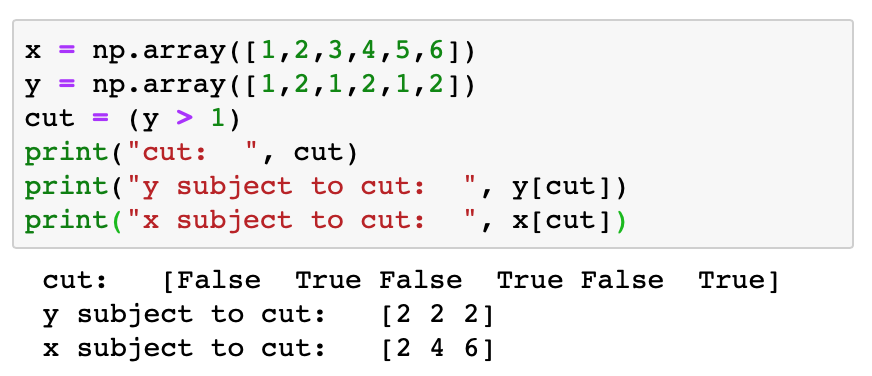
\includegraphics[width=0.65\textwidth]{figs//plotting/booleanmasks.png} 
\caption{Using boolean masks to cut on variable $y$.}
\label{fig:booleanmasks}
\end{center}
\end{figure}

A powerful technique in Scientific Python for performing analysis involving multiple variables uses boolean masks as shown in Fig.~\ref{fig:booleanmasks}.  In the example:
\begin{itemize}
\item Two numpy arrays $x$ and $y$ {\tt of the same length} are defined to contain the collected data.
\item The cut defined by $y > 1$ is a boolean array of the same length as $x$ and $y$ which is true at indices where the condition is met and false where it is not.
\item The subset of the entire $y$ array defined by {\tt y[cut]} consists only of those entries of $y$ for which the condition $y>1$ is met.
\item The subset of the entire $x$ array defined by {\tt x[cut]} consists only of those entries of $x$ for which the condition $y>1$ is met for the corresponding y value.
\end{itemize}
The last item shows the real power of this technique, one can look at one variable subject to constraints on another variable.

\begin{table}
\caption{Sample data for a voltage measurement subject to high frequency noise.}
\label{tbl:hfnoiseeg}
\begin{center}
\begin{tabular}{lll}
$t~(\rm s)$ & $v~(\rm V)$ & $n$ \\
0.4  & 0.25  &  2.8 \\
1.1  & 2.37  &  7.3 \\
1.4  & 1.69  &  9.7 \\
1.9  & 0.93  &  1.3 \\
2.5  & -1.0  &  6.2 \\
3.0  & 0.95  &  4.8 \\
3.4  & 1.22  &  6.9 \\
4.1  & 0.54  &  4.0 \\
4.4  & 0.37  &  1.9 \\
4.8  & 0.13  &  4.0 \\
5.5  & -2.04  &  9.5 \\
6.2  & -2.06  &  8.7 \\
6.5  & -0.81  &  2.3 \\
7.0  & -0.95  &  5.3 \\
7.5  & 0.98  &  9.7 \\
7.9  & 0.27  &  8.3 \\
8.5  & -0.81  &  0.1 \\
9.0  & -0.59  &  5.1 \\
9.4  & -0.37  &  4.4 \\
9.9  & 0.56  &  9.9 \\
\end{tabular}
\end{center}
\end{table}

Next consider the sample data in Table~\ref{tbl:hfnoiseeg} which comes from experimental measurements of a voltage level $v$ at discrete times $t$.  The measurement is subject to a high-frequency noise monitoring by the variable $n$.  The noise is only present for $n > 6.0$.  A straightforward way to load this data into scientific python is by defining numpy arrays for each variable as follows:
\begin{verbatim}
t = np.array([0.4, 1.1, 1.4, 1.9, 2.5, 3.0, 3.4, 4.1, 4.4, 4.8, 
                     5.5, 6.2, 6.5, 7.0, 7.5, 7.9, 8.5, 9.0, 9.4, 9.9])
v = np.array([ 0.25, 2.37, 1.69, 0.93, -1.0, 0.95, 1.22,   
                      0.54, 0.37, 0.13, -2.04, -2.06, -0.81, -0.95,  
                      0.98, 0.27, -0.81, -0.59, -0.37, 0.56])
n = np.array([2.8, 7.3, 9.7, 1.3, 6.2, 4.8, 6.9, 4.0, 1.9, 4.0,  
                      9.5, 8.7, 2.3, 5.3, 9.7, 8.3, 0.1, 5.1, 4.4, 9.9])
\end{verbatim}

\noindent
{\bf Plot 2} Prepare a plot of the sample data subject to the following:
\begin{itemize}
 \item Plot the voltage as a function of time as discrete data using red points.
 \item Define the boolean array {\tt keep} based on the noise reducing condition $n<=6.0$.
 \item Plot the voltage as a function of time, subject to the noise reducing condition using blue points.
 \item Plot the function $\sin(2 \pi x / 10)$ as a smooth function.
 \item Add appropriate axis labels.
 \item Add a legend for ``raw'' data with no cut, ``clean'' data with noise removed, and your continuous ``sin'' function.   
\end{itemize}
Your plot will reveal a clear sine function in the discrete data (after noise removal) consistent with the continuous function.  





\chapter{The Monte Carlo Method}

\section{Introduction}

This lab, which will take two lab sessions to complete, introduces the
Monte Carlo method, an approach to solving a wide range of problems by
repeatedly drawing random numbers from a probability distribution.
You will produce a sequence of pseudorandom numbers.  You will use a
histogram to directly compare values of random variables to a
probability distribution function.  With these preliminaries in hand,
you will explore several widely used Monte Calro techniques: Monte
Carlo integration, the rejection method, and the transform method.
You will finish by looking at the evolution of entropy during
diffusion, as modeled by a random walk.

\section{Generating random numbers}

The Monte Carlo method relies on the generation of random numbers, so
we will start there.  The numbers we generate using computers are
actually ``pseudorandom'' numbers, because they are deterministically
obtained from an algorithm.  However, the algorithm is choosen so that
the numbers appear random for practical purposes.  This is no small
concern.  Much of the computational work in the early 1970's had to be
redone because of the widespread use of a deeply flawed pseudorandom
number generator called RANDU.

In this section, you will generate a pseudorandom number sequence
using the linear congruential method.  This sequence is determined
iteratively from the simple relationship:
\begin{displaymath}
  I_{n+1} = (a*I_{n} + c) \mod M
\end{displaymath}
Recall that $x \mod y$ (coded as {\tt x \% y} in python) is the remainder
after integer division $x//y$.  Each $I_n$ is called a seed, and the
initial seed $I_0$ must be provided e.g. by the user.  Notice that the
seeds are all integers in the range from 0 to $(M-1)$.  If we wish to
convert these seeds into a random variable $x$ in the range from 0 to
$L$, we simply use $x_n = L * I_n / M$.  As long as $M$ is much larger
than $L$, $x$ is approximately continous.

The algorithm works because the product $a*I_{n}$ is generally many
times larger than $M$, so the remainder is effectively a uniform
random number.  The effectiveness of this algorithm is highly
dependend on the choice of $a$,$c$, and $M$.  Choose poorly and you get
RANDU.  Choose wisely and you get the highly regarded algorithm of
Park and Miller.  We will do the latter and use $a=7^5$, $c=0$, and $M
= 2^{31}-1$.

\begin{samepage}
\begin{plot} \end{plot}
Generate a sequence of ten uniform random variables in the range
$[0,1]$ from the Park-Miller sequence, using an initial seed of one.
Check your code by testing that the generator returns a {\bf seed} of
1043618065 after 10000 calls.  Change the initial seed to a value of
your choice and report the first 10 random values.  If you like, round
to two decimal places using {\tt np.around} to tidy up your output.
\end{samepage}

\section{Visualizing distributions}

\begin{figure}[htbp]
 \begin{center}
 \begin{tabular}{cc}   
  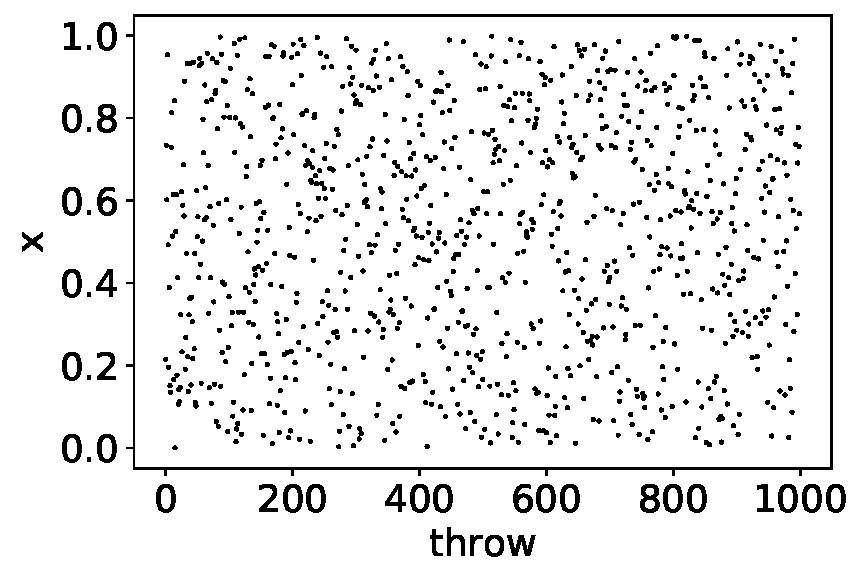
\includegraphics[height=0.22\textheight]{figs/labs/monte_carlo/flat2d.pdf} &
  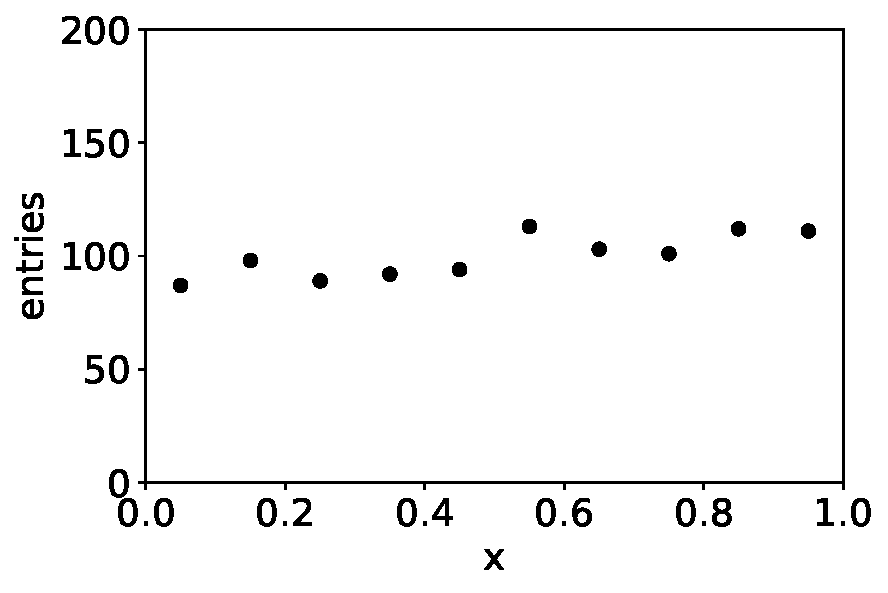
\includegraphics[height=0.22\textheight]{figs/labs/monte_carlo/flathist.pdf} \\
  (a) & (b) \\
 \end{tabular}
\caption{The (a) $x$ value of uniform random throws versus throw number and (b) corresponding histogram. }
\label{fig:flathist}
\end{center}
\end{figure}

\noindent
How can we verify that our Park-Miller random number generator
produces uniform random numbers in the range 0 to 1?  The associated
PDF is just $p(x)=1$, which we know how to plot, but how can we
compare this function to a sequence of numbers like $[0.21, 0.85,
  0.33, ...]$?  An initial attempt might look like
Fig.~\ref{fig:flathist}a, where we have simply plotted the $x$ value
of each throw versus the number of the throw.  Unfortunately, this
plot isn't particularly helpful.  If we zoomed in, we could determine
from the plot the $x$ value associated with each throw.  This is
simply too much information.

For interpreting a list of values as a distribution, there is only one
tool of choice: the histogram.  To histogram our data, we divide the
entire range $[0,1]$ into smaller ranges called {\em bins}.  Let's
start with 10 bins as an example. In this case, the first bin covers
the range from 0 to 0.1, or more precisely, the half-open interval
$\left[0,0.1\right)$ which includes $0$ and $0.099$, but not $0.1$.
  The second bin would have range $\left[0.1,0.2\right)$, the third
    bin would have range $\left[0.2,0.3\right)$ and so on, up to the
      last bin which would cover $\left[0.9,1.0\right]$.  To {\em
        fill} a histogram, you count the number of values that fall
      within the range of each bin.  So in our example, the value
      $0.21$ would add one to the count for the third bin, which has
      range $\left[0.2,0.3\right)$.  After filling, the histogram
        consists of a count associated with each bin range.

Fig.~\ref{fig:flathist}b shows a histogram filled with 1000 random
throws drawn from a uniform random number generator.  While we can now
see the shape of the distribution, we still don't have quite enough
information to answer the question, is this flat?  It is certainly not
perfectly flat!

The first feature we will need to add to the plot is the inclusion of
{\em error bars} to indicate the statistical uncertainty in our
histogram values.  Each histogram contains a {\em count} $n$ which
should follow a Poisson distribution with variance $\sigma^2 = n$.
Error bars are traditionally drawn with the size $\sigma$, which in
this case is $\sigma = \sqrt{n}$.  So when drawing a histogram, the
uncertainty in each bin is just the square root of the histogram
value.  That is the beauty of Poisson statistics!  If we have a count,
we know the statistical uncertainty.

\begin{figure}[htbp]
 \begin{center}
  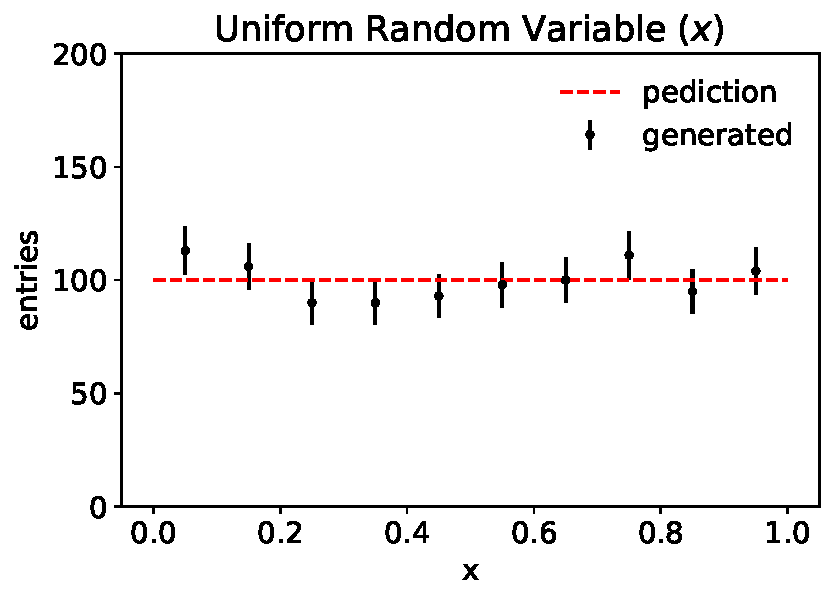
\includegraphics[width=0.50\textwidth]{figs/labs/monte_carlo/fancyhist.pdf}
  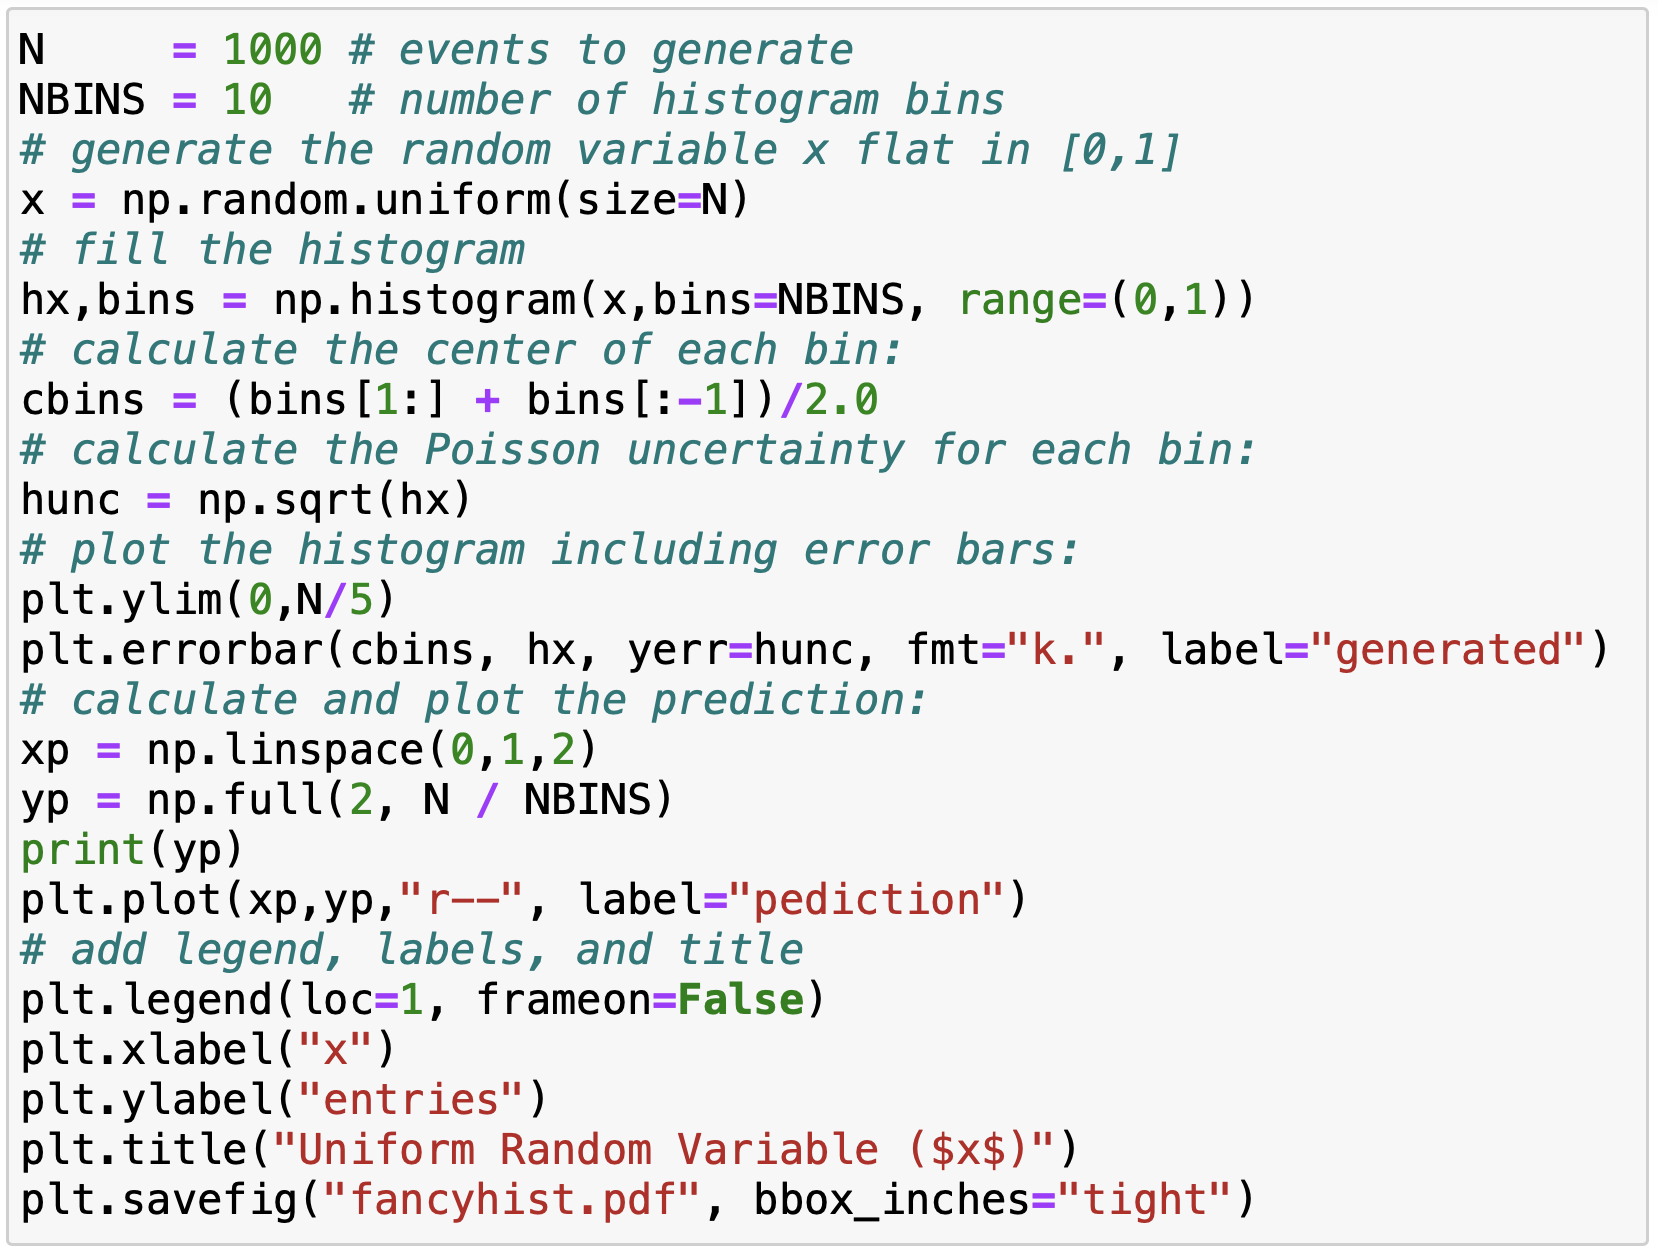
\includegraphics[width=0.75\textwidth]{figs/labs/monte_carlo/fancyhist-code.png}
\caption{Histogram of data drawn from a flat distribution compared to prediction, with the code used to produce the plot.}
\label{fig:fancyhist}
\end{center}
\end{figure}

We'll also want to add the prediction to the plot, assuming a flat
distribution for the contents of each bin.  In this case, we generated
$N$ events and we have $N_{\rm BINS}$ histogram bins, which should
therefore each contain an equal share: $N / N_{\rm BINS}$.  The
resulting histogram, along with the code used to generate it, is shown
in Fig.~\ref{fig:fancyhist}.  With the prediction and errorbars
included in the plot, one can now see that these generated values are
indeed quite consistent with a flat prediction. All of the bins are
within nearly one-sigma. With this number of bins, it is not uncommon
to see a two-sigma descrepancy.

You will produce many histograms in this class, so you will need to
(eventually) understand every single line in this example code.  Take
the time to read through the documentation for the key functions like
{\tt np.histogram} and {\tt np.random.uniform}, available on the web
(see numpy.org or just search ``np.histrogram python'').  A big part
of learning to program effectively, is learning how to read and
understand software documentation correctly and efficiently.

There are a few important features to notice:
\begin{itemize}
 \item The $x$-values are contained in an {\tt np.array} filled with
   uniform random variables generated by calling the {\tt
     np.random.uniform} function.
 \item The function {\tt np.histogram} is used to calculate a histogram
   from these $x$ values.  The call requests {\tt NBINS=10} histogram
   bins, in range $[0,1]$.  Don't confuse the python tuple {\tt (0,1)}
   used to indicate this range as indicating an open interval... often
   the computing language differs significantly from math notation, as
   is the case here!
 \item The {\tt np.histogram} function returns two items we need:  a {\tt np.array} containing the count for each bin ({\tt hx}) and a {\tt np.array} of bin edges ({\tt bins})
 \item We want to plot the count over the center of each bin, not one of the edges, so we calculate the quantity {\tt cbins} which is an {\tt np.array} containing the center of each bin.  You'll use this trick a lot, so make sure you understand what it is doing!
 \item The uncertainty on each bin {\tt hunc} is calculated as the square root of the bin counts {\tt hx}.
 \item We use the somewhat poorly named {\tt np.errorbar} function to plot {\bf both} the histogram central value {\tt and} the errorbar in each bin.
 \item We draw the prediction as a straight line defined by two points defined by {\tt xp} and {\tt yp}.
\end{itemize}

\begin{plot} \end{plot}
Modify the example code to generate a histogram for uniform random
numbers generated from your Park-Miller sequence instead of ${\tt
  np.random.uniform}$.  Increase the number of events to {\tt
  N=10000}.  Increase the number of bins to {\tt NBINS=20}.  Does your
code appear to produce uniform random numbers?

To answer a question in your notebook, simply add a cell and answer the question as a comment (each line starting with {\tt \#}).

\section{Calculating the value of $\pi$}

\begin{figure}[htbp]
\begin{center}
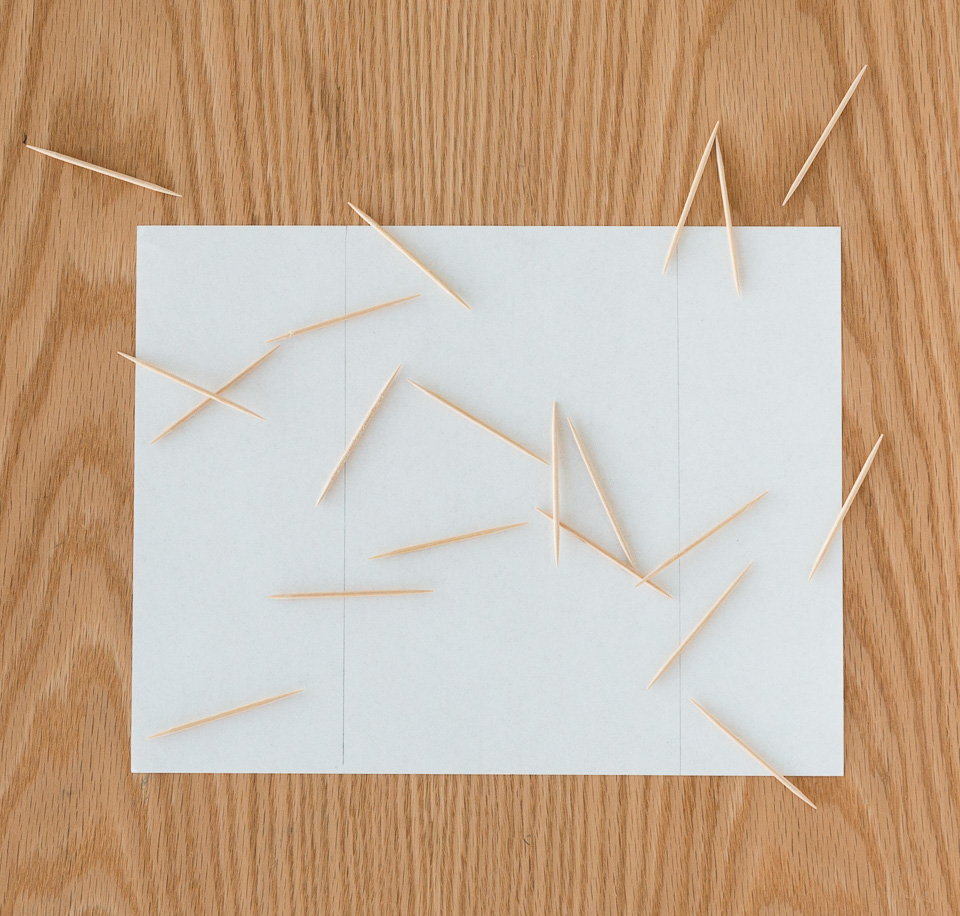
\includegraphics[width=0.65\textwidth]{figs/labs/monte_carlo/pitoss.jpg} 
\caption{Determining $\pi$ by throwing toothpicks.}
\label{fig:pitoss}
\end{center}
\end{figure}

\noindent
Hopefully 2021 will see the return of parties, so let's start by
examing a surefire way to be the life of the party: determining the
constant $\pi$ by throwing toothpicks!  The procedure is simple: you
cut a peice of paper to a width of four toothpicks, then draw two
vertical lines separated by the width of two tooth picks.  Take turns
tossing toothpicks, as in Fig.~\ref{fig:pitoss}.

From the geometry of the setup, it can be shown that the probability
that a toothpick which is entirely on the paper also crosses a line is
given by $1/\pi$.  Therefore, one can measure $\pi$ by counting the
total number of toothpicks that landed entirely on the page and
dividing by the number of those toothpicks that crossed a line.  This
is, in essence, the Monte Carlo method.

\begin{figure}[htbp]
\begin{center}
  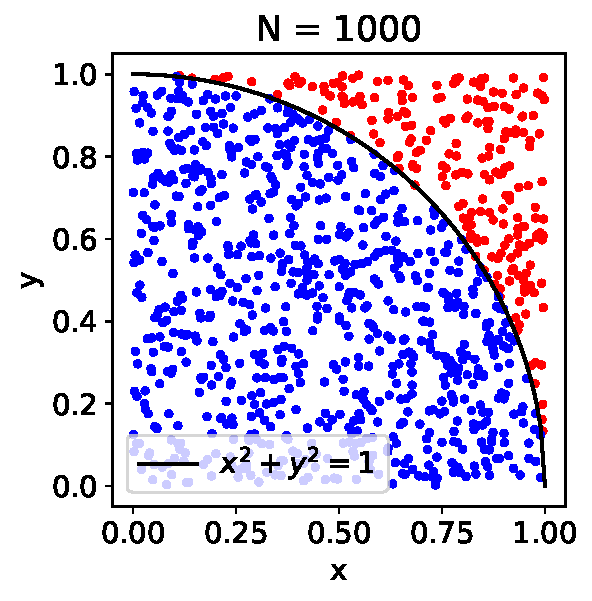
\includegraphics[width=0.50\textwidth]{figs/labs/monte_carlo/pimc.pdf}
  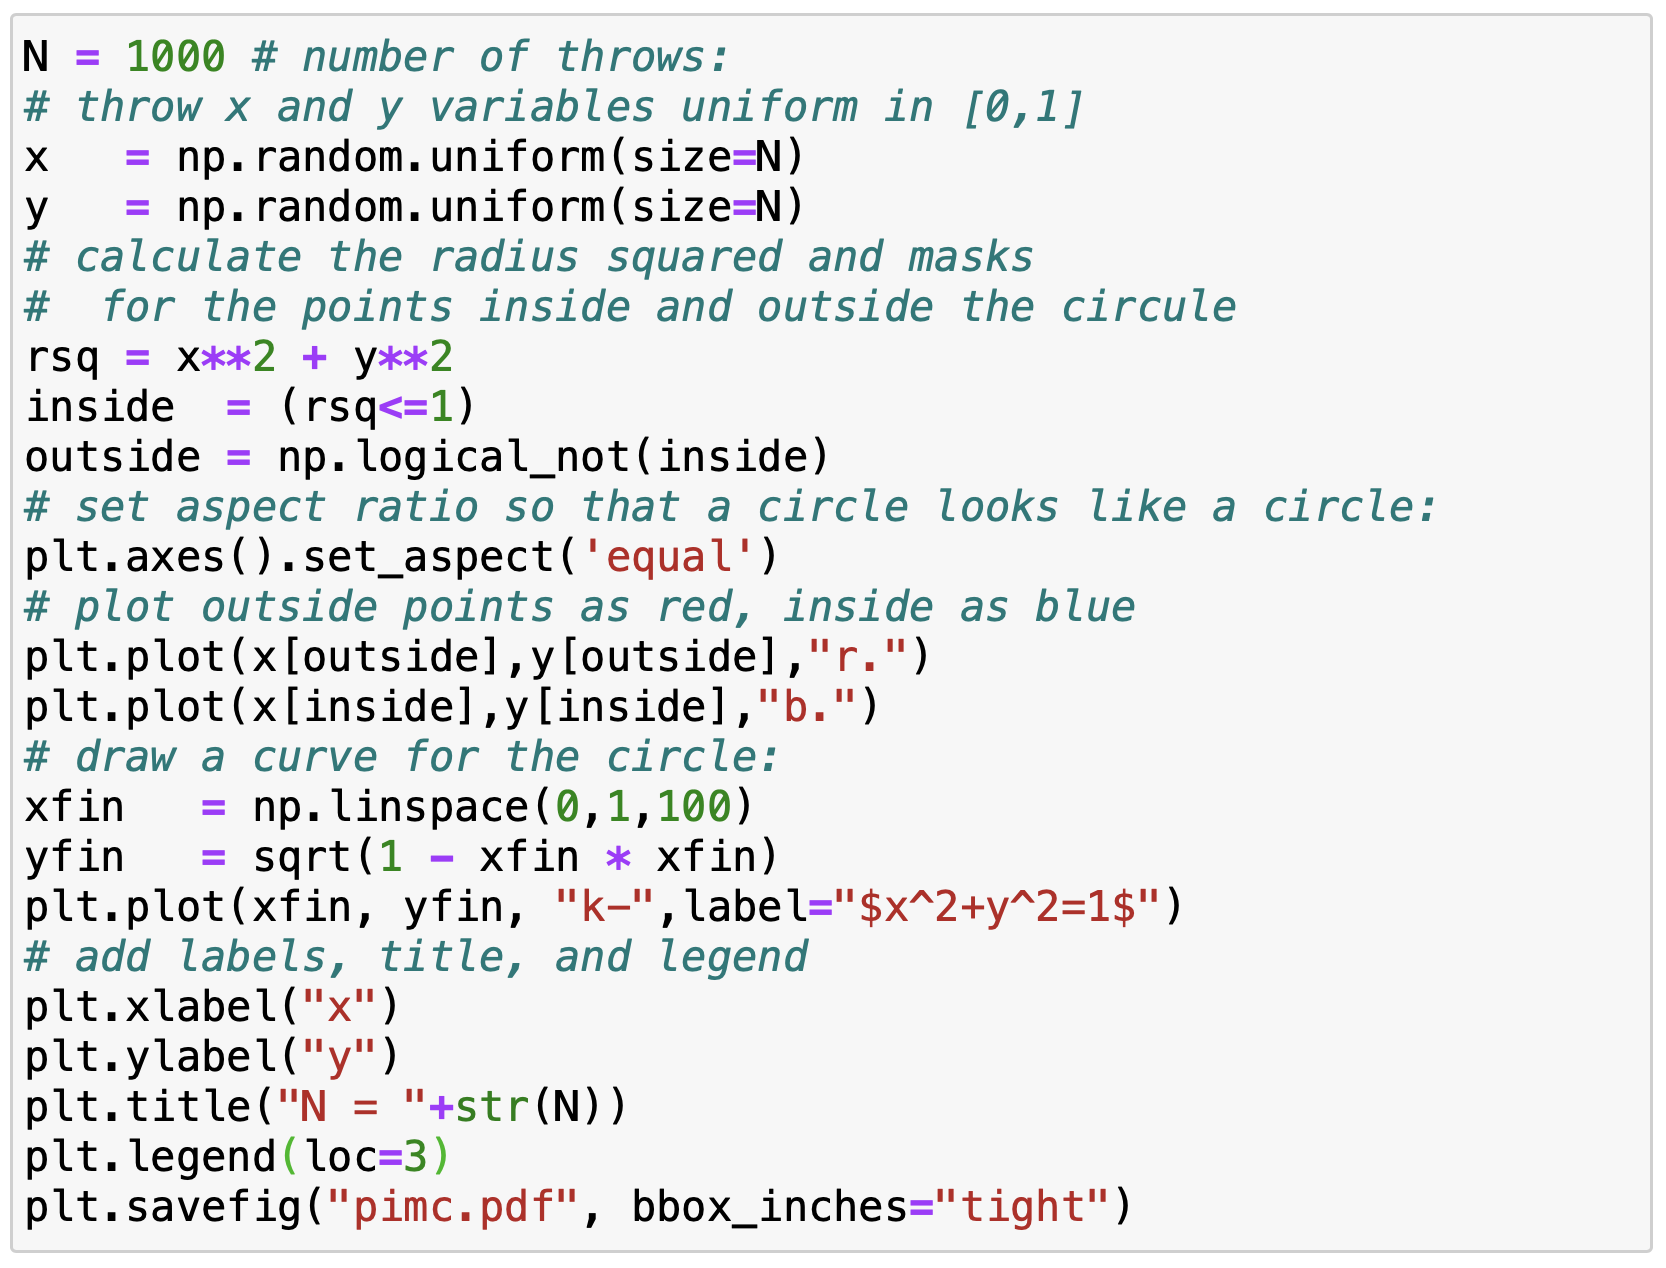
\includegraphics[width=0.75\textwidth]{figs/labs/monte_carlo/pimc-code.png} 
\caption{Monte Carlo Determination $\pi$ .}
\label{fig:pimc}
\end{center}
\end{figure}

An easier Monte Carlo method to implement computationally is shown in
Fig.~\ref{fig:pimc} along with the code used to generate the plot.
The idea is to throw points uniformly in the unit square of area 1.
Much like in the toothpick example, the value of $\pi$ can be
determined by counting the number of generated points that also landed
within the unit circle.

The key features of the example code are:
\begin{itemize}
\item The $x$ and $y$ values are each contained in an {\tt np.array} filled with uniform random variables in $[0,1]$ by the {\tt np.random.uniform} function.
\item A mask {\tt inside} is created to indicate which points are inside the circle.  Recall that the mask is an {\tt np.array} of True or False values, with the same length as the $x$ and $y$ arrays.  For example {\tt x[inside]} is an np.array containing just the subset of {\tt x} which are inside the circle.  
\end{itemize}

\begin{plot} \end{plot}
Starting from the example code, determine the numerical value of $\pi$
using the Monte Carlo method.  The easiest way to obtain the count you
need is to apply the function {\tt np.sum} to an appropriate mask.
When counting a mask, each True is treated as a one, and each False is
treated as zero.  Work out the relationship between $\pi$ and the
fraction of events in the unit circle, and use your count to
numerically determine the value of $\pi$.  Increase the number of
generated events and confirm that your calculated value of $\pi$
approaches the known value.

\begin{plot} \end{plot}
This is an example of a binomial process, because points are either
inside or outside the circle. So we expect the number of events in the
circle to follow the binomial distribution with $\sigma^2 = n \epsilon
(1-\epsilon)$.  In this case, $n$ is the total number of generated
events and $\epsilon$ is the fraction that fall inside the unit
circle.  The statistical uncertainty on your measured value of $\pi$
works out to be:
\begin{displaymath}
\sigma_\pi = \sqrt{\frac{\pi \, (4-\pi)}{n}}
\end{displaymath}
where $n$ is the number of generated events.  Does your measured value
of $\pi$ agree with the known value within your statistical
uncertainty?

\section{Monte Carlo integration}

The Monte Carlo method can also be used to numerically integrate a
function.  Monte Carlo integration methods generally only outperform
deterministic methods when the number of dimensions is large, but we
can illustrate the method most easily in one dimension. In this
section, you'll use the Monte Carlo method to perform the integral:
\begin{displaymath}
  \int_0^\pi \sin^2 \theta \, d\theta
\end{displaymath}

To do so, you should make a copy of your solution from the previous section
and modify it in the following manner:
\begin{itemize}
 \item Instead of thowing $x$ in $[0,1]$, throw $\theta$ in $[0,\pi]$.  This means the area of the rectangle $A$ is now $\pi$ instead of 1.
 \item Count the number of throws that land below the integral $y < \sin^2 \theta$.
 \item Determine the area under the curve as the fraction of the throws under the curve times the total area of the rectangle $A$.
 \item The statistical uncertainty in this case is $\pi/(2\sqrt{n})$ where $n$ is the number of generated events.
\end{itemize}  

\begin{plot} \end{plot}
Use the Monte Carlo method to calculate the integral:
\begin{displaymath}
  \int_0^\pi \sin^2 \theta \, d\theta
\end{displaymath}
Make a plot similar to that of Fig.~\ref{fig:pimc} showing the thows
above the curve in red and below the curve in blue.  Calculate the
integral and statistical uncertainty and compare it to the value you obtain analytically.

\section{The Rejection method}

\begin{figure}[htbp]
\begin{center}
  \begin{tabular}{cc}
  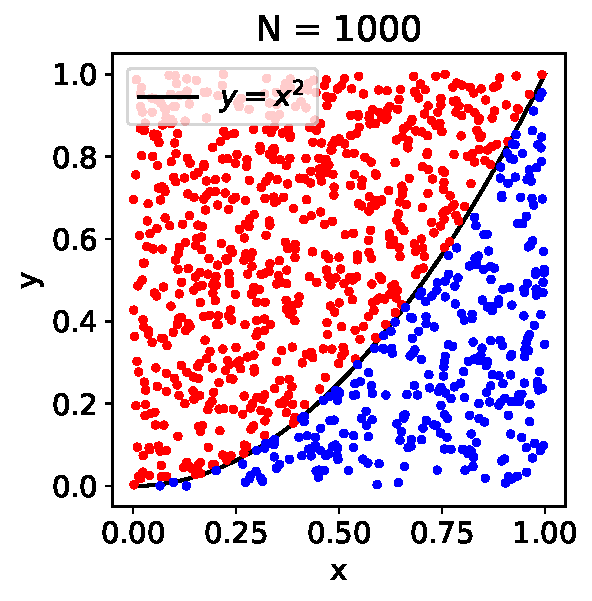
\includegraphics[height=0.30\textheight]{figs/labs/monte_carlo/rejectmc.pdf} &
  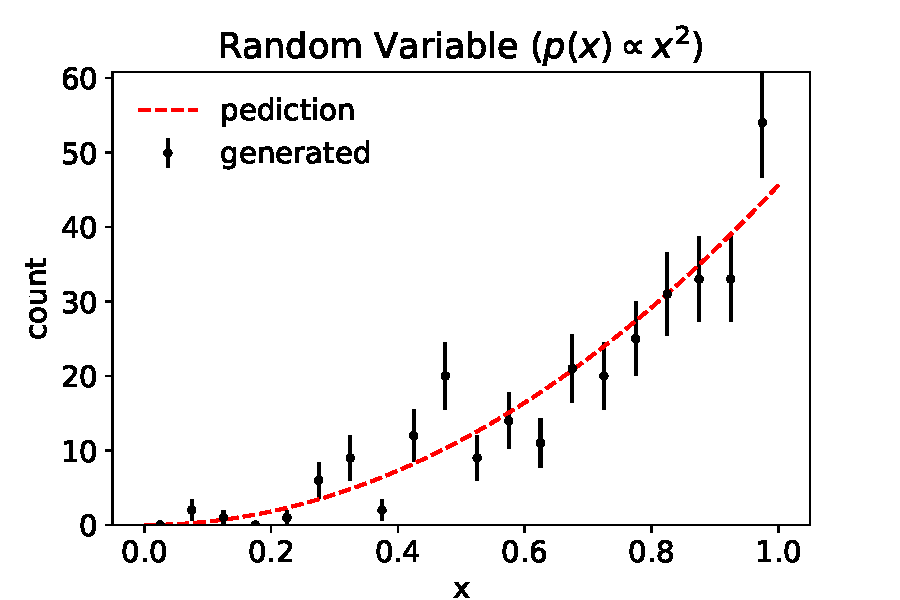
\includegraphics[height=0.30\textheight]{figs/labs/monte_carlo/quadhist.pdf} \\
  (a) & (b) \\
 \end{tabular}
  \caption{Monte Carlo rejection method applied to $p(x) \propto
    x^2$. Uniformly generated points (a) are rejected (red) if they
    are above the PDF, and the $x$ values of points below the PDF
    (blue) are selected.  A histogram (b) of the selected $x$ values
    shows that they follow the PDF.}
  \label{fig:rejectmc}
\end{center}
\end{figure}

\noindent
We now know how to generate uniform random numbers, but suppose we
need a random variable thrown according to a non-uniform probability
distribution $p(x)$?  Fig.~\ref{fig:rejectmc} demonstrates one
approach, which closely follows the procedure for numerical
integration using the Monte Carlo technique.

The rejection method produces random variables in a range from 0 to $L$
according to any desired PDF $p(x)$.  Start by finding a value $Y$ which is at
least as large as the maximum value of $p(x)$ for $x$ in $[0,L]$.  Then:
\begin{itemize}
  \item Throw $x$ as a uniform random variable in range $[0, L]$.
  \item Throw $y$ as a uniform random variable in range $[0, Y]$.
  \item If $y > p(x)$ reject the $x$ value and start over, otherwise, use the $x$ value as one throw.
\end{itemize}
Repeat these steps as necessary until a sufficent number of $x$ values have been selected.

The rejection method works because the probability of an $x$ value
being selected is, by construction, proportional to $p(x)$.  Since the
$x$ values were initially chosen from a flat distribution, the
selected $x$ values will follow the $p(x)$ distribution.  You can
visualize this in Fig.~\ref{fig:rejectmc} which leaves very little
doubt that the $x$ values of the blue points will follow the PDF.
Notice that it isn't even necessary for $p(x)$ to be normalized for
this procedure to work: any function proportional to the PDF of interest will do.

To produce a smooth function such as the quadratic prediction of
Fig.~\ref{fig:rejectmc}b, make sure you use plenty of $x$ values
(around 100 at least), via {\tt np.arange} or {\tt np.linspace}, just
as you did in the Plotting lab.  When comparing a PDF to histogrammed
data (as you will do for the second plot below) you will need to
normalize it appropriately.  The number of throws we expect to find in
a bin with edges at $a$ and $b$ is given by
\begin{displaymath}
  N \cdot \int_a^b p(x) \, dx \; = N \cdot p(x^*) \cdot (b-a) 
\end{displaymath}
The integral is simply the probability that one throw ends up in the
range, which we scale by the total number of throws $N$.  The equality
holds for at least one $x^*$ in the range $[a,b]$ and $(b-a)$ is
simply the bin size.  Therefore, we can formulate a prediction from a
normalized PDF $p(x)$ to data from $N$ throws used to fill a histogram with
bin sizes $\Delta x$ as the smooth function resulting from:
\begin{displaymath}
N \cdot p(x) \cdot \Delta x
\end{displaymath}
This is a technique we will use over and over again, so make sure you
understand it!

\begin{plot} \end{plot}
Use the rejection method to generate random numbers in the region from [0,1] that follow a distribution $p(x) \propto x^2$.  You'll do the following:
\begin{itemize}
  \item Note that there is no need to normalize the PDF when using the rejection method, so use $p(x)=x^2$.
  \item In our $x$ range $[0,1]$, $p(x)$ has maximum value at $x=1$ so set $Y = p(1) = 1^2 = 1$. 
  \item Throw $x$ as a uniform random variable in the range $[0, 1]$.
  \item As $Y=1$, throw $y$ as a uniform random variable in range $[0, 1]$.
  \item If $y > x^2$ reject the $x$ value and try a new set of $x$ and $y$ values, otherwise, use the $x$ value as one throw.
\end{itemize}
Throw 1000 (unselected) $x$ values, and produce a plot like that of
Fig.~\ref{fig:rejectmc}a showing your selected points in blue, your
rejected points in red, and the selection function ($p(x) = x^2$).

\begin{samepage}
\begin{plot} \end{plot}
Increase the number of (unselected) $x$ values thrown to 10,000.
Count the number $N$ of selected $x$ values.  Generate a plot like that of
Fig.~\ref{fig:rejectmc}b comparing the distribution of your selected
$x$ values to the prediction, which in this case is given by:
\begin{displaymath}
N \cdot 3x^2 \cdot \Delta x
\end{displaymath}
Be careful to use the number of selected $x$ values for $N$, not the total thrown (10000) before rejection.
\end{samepage}

\section{The transformation method}

Suppose that you need to throw random variables according to an
exponential distribution $p(x) = \exp(-x)$.  This PDF is defined for
$[0,+\infty)$ and properly normalized across this range as you can verify:
\begin{displaymath}
  \int_0^{+\infty} \exp(-x) \, dx = 1
\end{displaymath}    
The first problem is that we can only generate uniform random
variables up to a finite value $L$, not $+\infty$.  But let's suppose we are
willing to work aound this by simply cutting off the PDF at some large
value, like say we won't produce values with $x>100$.

With this change, the rejection method will work in principle.  But it
still has a major shortcoming.  Since $p(x)$ has a maximum value of 1,
and $x$ ranges from 0 to 100, the rectangle we will be filling with
uniform random points has area 100.  But our PDF, even when
integrated to $+\infty$, only has area 1.  So less than one out of
every 100 points we throw will be selected.  Perhaps we can live with
this, but then what if we need to go out to $x=1000000$.  Now only one
out of every million points will be selected.  In many scenarios, the
rejection method becomes too computationally inefficient to be of any
practical value.

In these case, we can use the transformation method instead of the
rejection method.  The transformation method is premised on the fact
that for {\em any} normalized PDF, we must have
\begin{displaymath}
  p(x) \geq 0
\end{displaymath}
everywhere and
\begin{displaymath}
  \int_{-\infty}^{+\infty} p(x) \; dx = 1
\end{displaymath}
as long as we take care to set $p(x)=0$ outside our range for $x$.  It follows from these properties that for any value of $y$ in the range $[0,1]$ there is a unique largest $x$ value for which:
\begin{equation} \label{eqn:mctransform}
  \int_{-\infty}^{x} p(x) \; dx = y
\end{equation}
From the fundamental theorem of calculus, we see that:
\begin{displaymath}
  dy = p(x) \, dx
\end{displaymath}
If the variables $y$ are drawn from a uniform distribution with PDF $q(y)=1$, then we see that:
\begin{displaymath}
 \int_{y_1}^{y_2} q(y) \, dy = \int_{x_1}^{x_2}p(x) \, dx.
\end{displaymath}
for $x_i$ and $y_i$ related by Eqn.~\ref{eqn:mctransform}.  This shows
that while $y$ is a uniform random variable ($q(y)=1$), the
corresponding $x$ values will distributed according to the desired PDF
$p(x)$.

That provides the mathematical justification for the transformation
method, which starts by finding the inverse function $f^{-1}(y)$ for:
\begin{displaymath}
  y = f(x) = \int_{-\infty}^{x} p(x) \, dx
\end{displaymath}
Then the procedure is:
\begin{itemize}  
 \item Throw $y$ as a uniform random variable in $[0,1]$.
 \item Find $x = f^{-1}(y)$
\end{itemize}
The $x$ values determined in this way will be drawn from the $p(x)$ distribution.  

There is an intuitive explanation for why this works.  The $y$ value is
essentially a fraction of the probability integrated by the PDF.  In a
region of $x$ where $p(x)$ is relatively large, the integral is
changing rapidly and so a large range of $y$ values map to this region
of $x$-values.  In a region of $x$ where $p(x)$ is relatively small,
the integral is not changing rapidly and so a small range of $y$
values map to this region of $x$-values.

Let's see how this applies to our exponential function.  In this case we calculate:
\begin{displaymath}
y = f(x) = \int_0^x \exp(-x) \, dx = 1 - \exp(-x)
\end{displaymath}  
which we invert to find:
\begin{displaymath}
x = - \ln(1-y)
\end{displaymath}  
To determine values of the random variable $x$, we follow this procedure:
\begin{itemize}
 \item Throw a $y$ value flat in [0,1]
 \item Caculate $x = -\ln(1-y)$
\end{itemize}
Repeat to produce as many $x$ values as needed.  Notice that this
procedure gives one usable $x$ value for every random throw.

\begin{plot} \end{plot}
Use the transformation method as described to generate 10,000 values
of a random variable thrown from an exponential function.  Produce a
plot like that of of Fig.~\ref{fig:rejectmc}b comparing the
distribution of your generated events to the prediction for $p(x) =
\exp(-x)$.  Remember to properly normalize your prediction based on
the bin size and number of events thrown.

\newpage
\section{Particle diffusion}

\begin{figure}[htbp]
\begin{center}
  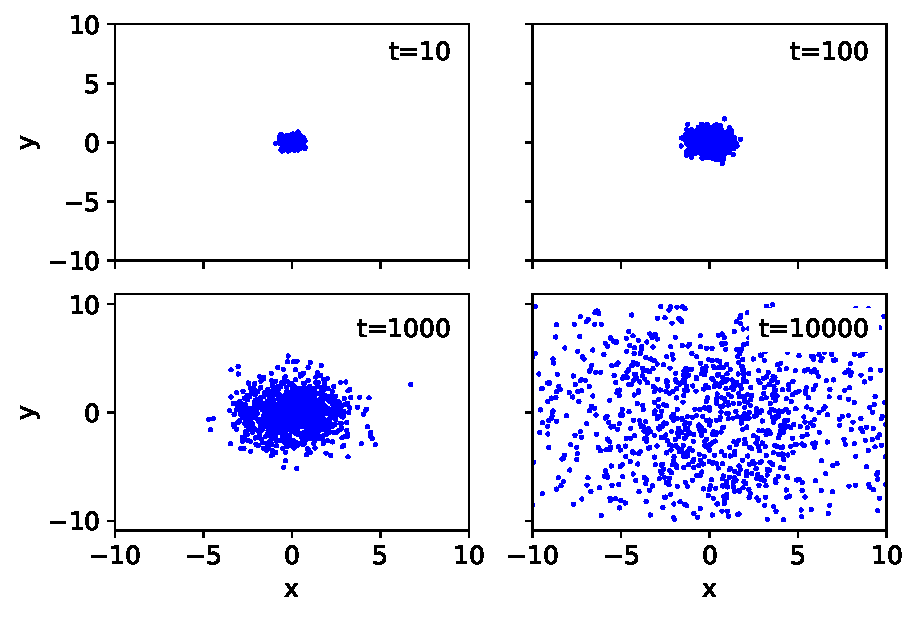
\includegraphics[width=0.80\textwidth]{figs/labs/monte_carlo/diffusion.pdf}
  \caption{Simulation of the diffusion of a drop of particles at four different times.}
\label{fig:diffusion}
\end{center}
\end{figure}

\begin{figure}[htbp]
 \begin{center}
  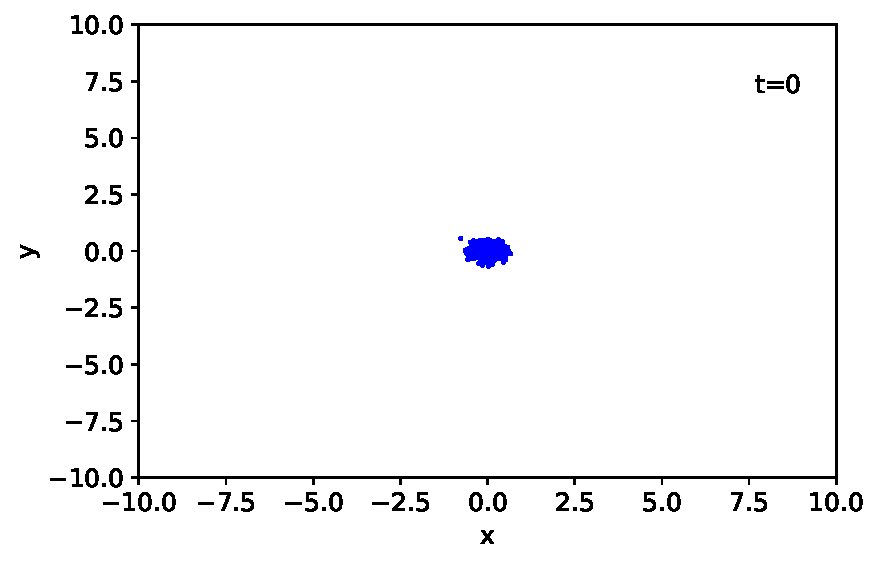
\includegraphics[width=0.50\textwidth]{figs/labs/monte_carlo/diffstart.pdf}
  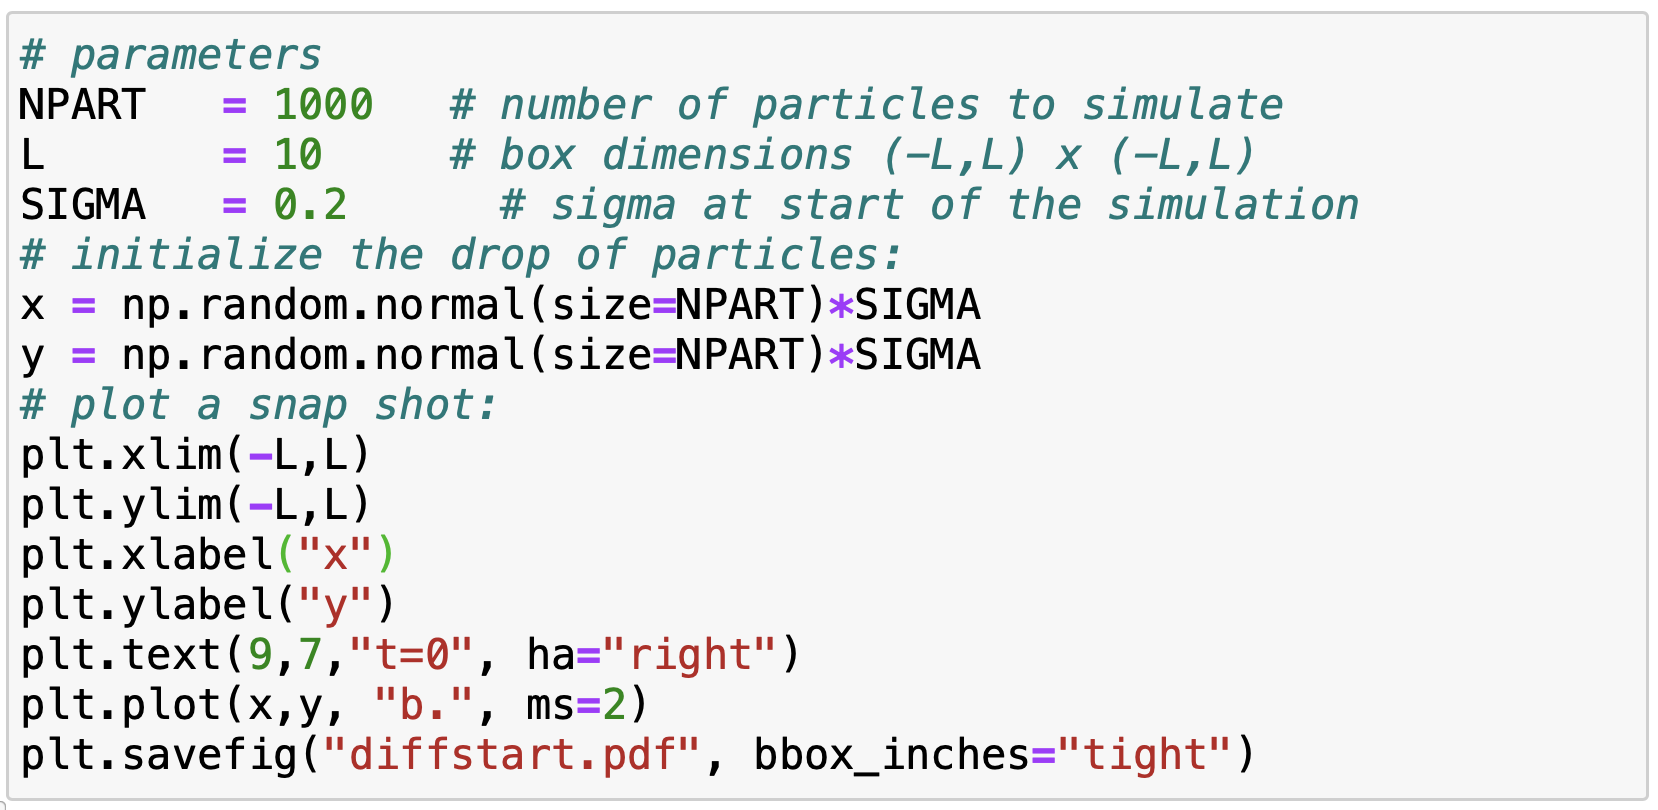
\includegraphics[width=0.75\textwidth]{figs/labs/monte_carlo/diffstart-code.png}
  \caption{Snapshot of the simulation at the start, along with the code used to produce it.}
\label{fig:diffstart}
\end{center}
\end{figure}


\noindent
In this section, we will model the diffusion of a drop of particles in
a medium, as in Fig.~\ref{fig:diffusion}, shown as snapshots at four
different times.  The starting point for the simulation, at $t=0$ is
shown in Fig.~\ref{fig:diffstart} along with the code used to produce
it.  The entire state of the system is contained in the arrays {\tt x}
and {\tt y} which contain the $x$ and $y$ positions of each particle.

The diffusion process is modeled by a random walk. During each update
(for one time step) the $x$ and $y$ values of each particle should be
randomly increased or decreased by an amount {\tt STEP=0.2} Any
particles that would leave the boundaries of the region $[-L,L]$ as a
result should be moved back into the region.  The numpy functions 
{\tt np.random.choice} and {\tt np.clip} are useful here.

Despite the symmetry of the random walk, the system clearly evolves by
diffusing outward over time.  This can be seen as a consequence of the
second law of thermodynamics.  Calculating the entropy from the
microscopic state of continuous particles is a bit tricky.  The
approach we will use is based on the Gibb's entropy.  We divide the
area into cells, and determine the fraction of the particles $f_i$ in
each cell $i$.  We calculate the entropy as:
\begin{displaymath}
  S = \sum_i f_i \ln f_i
\end{displaymath}
A python function which calculates the entropy in this manner:
\begin{tt}
\begin{verbatim}
from scipy import stats  
def entropy(x,y,l,sbins):
    h,xbins,ybins=np.histogram2d(x,y,bins=sbins,range=[[-l,l],[-l,l]])
    return stats.entropy(h.flatten())
\end{verbatim}
\end{tt}
The function takes as input parameters the position arrays {\tt x} and
{\tt y}, the boundary distance {\tt l} (set it to {\tt L} and the
number of bins in each dimension {\tt sbins} (set it to 20).  The
function returns the entropy of the current state of the system
described by {\tt x} and {\tt y}.

\begin{plot} \end{plot}
Starting from the example code, implement a random walk to model the
diffusion process, and plot four snap shops showing the evolution of
the system.

\begin{plot} \end{plot}
Calculate and record the entropy of the system as it evolves, and plot
the entropy as a function of time.


\chapter{Limits of Distributions}

\section{Introduction}

In this lab, we will use a Monte Carlo simulation to demonstrate the
convergence of statistical distributions.  We'll see that the binomial
distribution approaches the Poisson distribution for a large number of
trials, and that the Poisson distribution approaches the Gaussian
distribution for a large values of the mean value $\lambda$.  You will
produce your own numerical demonstration of the Central Limit Theorem,
by considering the average value of uniform random variables.

\section{Poisson Limit of the Binomial Distribtion}

We showed in lecture that the Binomial distribution for $n$
independent trials with success probability $\epsilon$ approaches a
Poisson distribution with mean value $\lambda = \epsilon \cdot n$ as $n\to
\infty$.  We will demonstrate this numerically by using a large but
finite value for the number of trials $n$.

A simulation of a binomial process is demonstrated in
Fig.~\ref{fig:binom} which will be a good start for the exercises.
While working through the example, note a few key features:
\begin{itemize}

\item Note the distinction between the number of trials {\tt NTRY} and
  the number of random throws {\tt THROWS}.  The simulation throws
  {\tt THROWS} random variables $m$ each of which represents the
  outcome of an binomial process with {\tt NTRY} trials.  It's easy to
  get these quantities confused!

\item The simulated binomial outcomes are contained in the array {\tt
  m} which is filled by calling the \\ {\tt np.random.binomial}
  function which is designed for this specific purpose.  It produces
  an array of the specified size containing values randomly drawn from the
  binomial distribution with {\tt n} trials of {\tt p} success probability.
  Here the computing languages uses {\tt p} for the parameter we call
  $\epsilon$.  That's life!

\item We want to keep the parameter $\lambda$ constant as we vary $n$ so we set the success probability $\epsilon = \lambda / n$ with the line {\tt EPS = LAMBDA / NTRY}.

\item We calculate and plot a histogram in much the same way as in
  previous exercises.  But notice that instead of center of each bin,
  we bplot using the left edge of each bin, determined as {\tt lbins =
    bins[:-1]}.  The reason for this choice is described in more
  detail below.

\item We compare our simulated outcomes to the probability mass function (PMF) for the Binomial process evaluated at the integer values in the array {\tt lbins}

\item The prediction for each bin is normalized by multiplying the PMF (which represents a single throw) by the number of throws {\tt THROWS}.  There is no factor for the bin size in this normalization, because the bin size is 1.

  
\end{itemize}

{\bf Binning integer data:} when plotting a histogram filled from
continuous data, we plotted the count for each bin over the central
$x$ value for the bin.  So the number of entries in the range $[0,1)$
would be plotted over the value $0.5$.  This is a good choice for
continuous data, because continuous data fills the entire range
$[0,1)$.  But in this example, our random variables are integers.  The
only value that can increment the bin at $[0,1)$ is the value
(the range is open on the right, and does not include 1, which is left
for the next bin!)  In this case, it is misleading to plot a count
of the value 0 over the center of the bin at 0.5.  Instead, when
plotting histograms of integer data with integer bins, we plot the
data over the left edge of the bin.  For example, the count of 0
values will be placed directly over 0.

\begin{samepage}
\begin{plot} \end{plot}
Adjust the example code so that the simulated binomial process is
compared to the Poisson PMF instead of the binomial PMF.  Look up the
{\tt np.stats.poisson.pmf} function.  {\bf Make sure that you leave
  the simulation unchanged:} the point of this exercise is to simulate
a binomial process but compare it to a Poisson PDF.  Leave the number
of trials (and other parameters) unchanged.  The agreement between the
Binomial simulation and the Poisson PDF should not agree for six
trials.  Do your results here confirm that?
\end{samepage}

\begin{samepage}
\begin{plot} \end{plot}
Increase the number of trials in your simulated process to 100.  Does
your binomial process now resemble a Poisson PDF?
\end{samepage}

\begin{figure}[htbp]
\begin{center}
  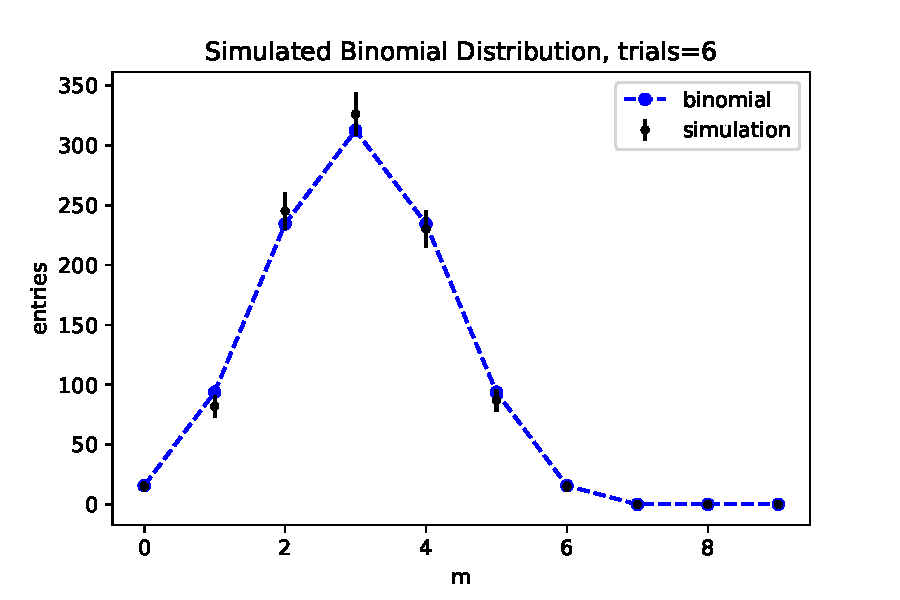
\includegraphics[width=0.50\textwidth]{figs/limits/binomial.pdf}
  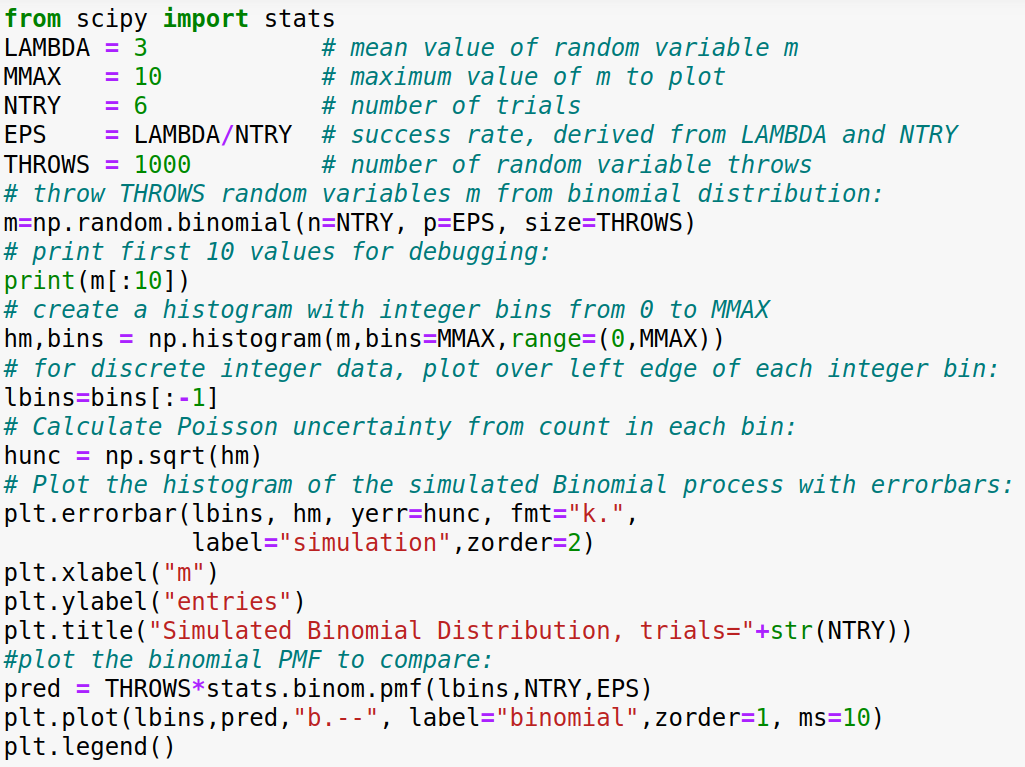
\includegraphics[width=0.75\textwidth]{figs/limits/binomial-code.png} 
\caption{Simulation of a binomial process.}
\label{fig:binom}
\end{center}
\end{figure}

\section{Gaussian Limit of the Poisson Distribtion}

We discussed in lecture that in the limit $\lambda \to \infty$, the
Poisson distribution will approach a Gaussian distribution with mean
value $\lambda$ and $\sigma = \sqrt{\lambda}$.  We will demonstrate
this result numerically using a simulated Poisson process and a large
but finite value of $\lambda$.

A simulation of a Poisson process is demonstrated in
Fig.~\ref{fig:poisson}, which is similar in many respects to the
previous example.  Note a few features:
\begin{itemize}
\item The simulated Poisson outcomes are contained in the array {\tt
  m} which is filled by calling the \\ {\tt np.random.poisson}
  function which is designed for this specific purpose.  It produces
  an array of the specified size containing values drawn from the
  poisson distribution with mean {\tt lam} (the parameter we call
  $\lambda$).

\item The $x$-values used as locations to plot the histogram counts
  are contained in the array {\tt ibins}.  These are determined from
  the bin edges as the largest integer smaller than the center of the
  bin.  This reduces to the left edge for integer bins (as in the
  previous example) but will continue to work as the bin size
  increases to include multiple integers.

\item The outcomes are now being compared to the continuous Gaussian
  PDF.  For this reason, a finely binned set of of $x$-values are
  contained in the {\tt xf} array, filled using the {\tt np.linspace}
  function.  This will plot a nice smooth function, appropriate for a
  continuous function.
  
\item The prediction is normalized by multiplying the PDF (which
  represents a single throw) by the number of throws {\tt THROWS} and
  the bin size.  The bin size factor is needed because we are using a
  probability density function and the bin size will be different than
  one in the exercises.

\item The parameters for the Gaussian PDF are poorly choosen in the
  example, on purpose.
\end{itemize}

\begin{plot} \end{plot}
Lookup the function {\tt scipy.status.norm.pdf}.  Set the parameters
{\tt loc} and {\tt scale} to values consistent with the simulation.
Leave $\lambda=3$ for now and plot your results.  How does the Gaussian distribution compare to Poisson distribution at $\lambda=3$?

\begin{plot} \end{plot}
Now set $\lambda=100$.  Adjust the range for plotting to $[70,130]$ and set the number of bins to 20.
The Gaussian distribution distribution should agree closely with the Poisson distribution at this point.  Is that what your simulation shows?

\begin{figure}[htbp]
\begin{center}
  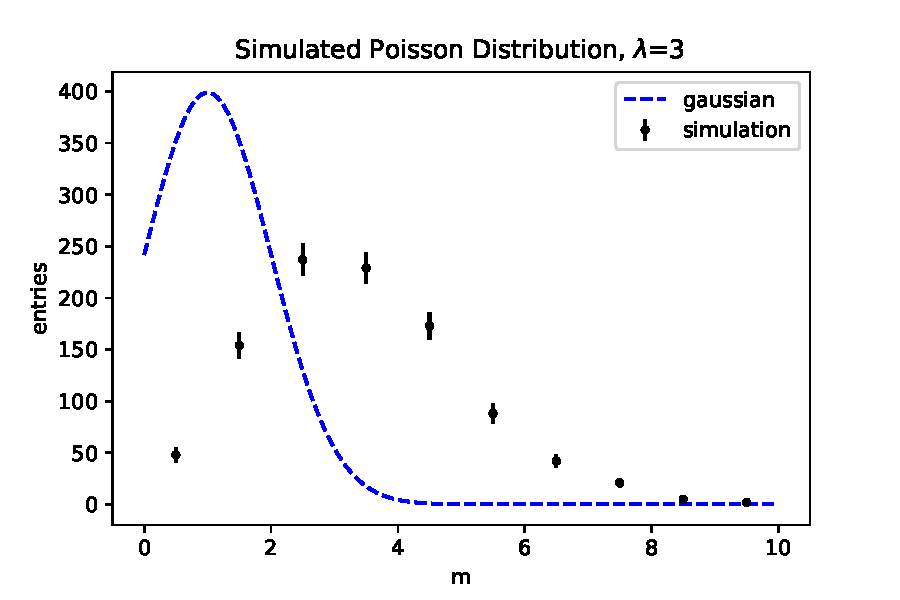
\includegraphics[width=0.50\textwidth]{figs/limits/poisson.pdf}
  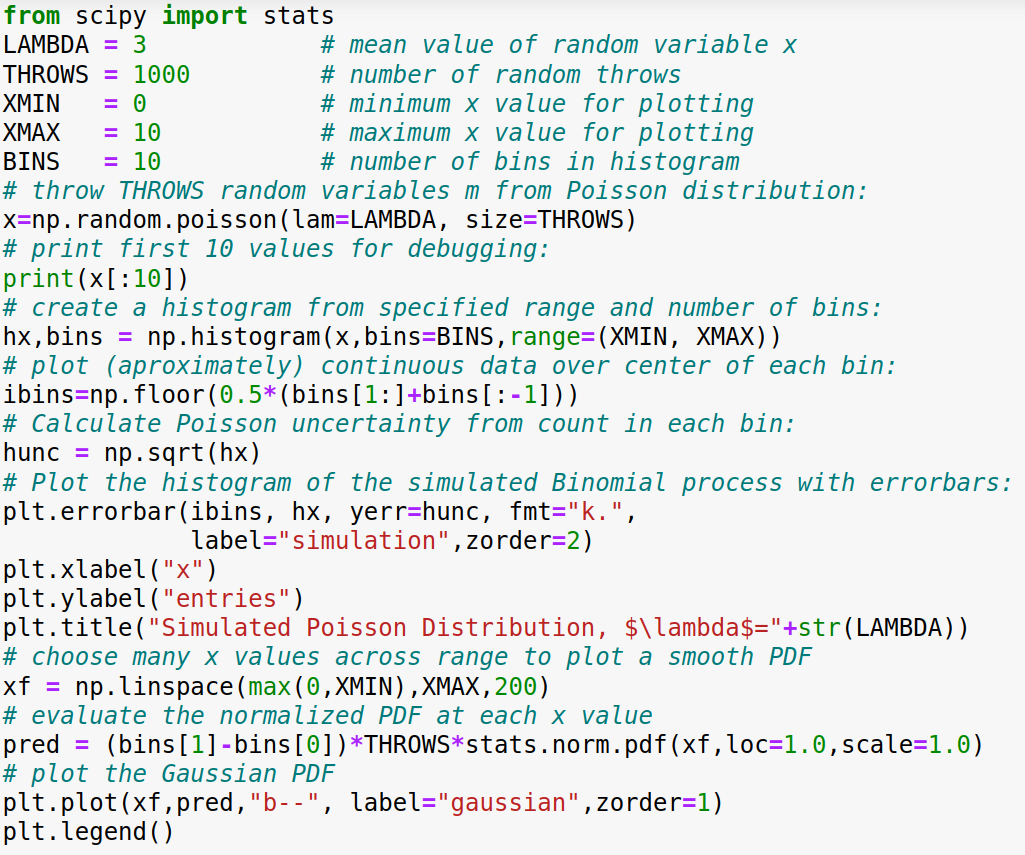
\includegraphics[width=0.75\textwidth]{figs/limits/poisson-code.png} 
\caption{Simulation of a binomial process.}
\label{fig:poisson}
\end{center}
\end{figure}


\section{The Central Limit Theorem}

The central limit theorem states that a properly normalized sum of
independent random variables will tend toward the Gaussian
distribution, even if the random variables are drawn from a different
distribution.  In this section, you will demonstrate this fact by
showing that the average of {\tt NSUM} uniform random variables does
in fact follow a Gaussian distribution.

When solving these exercises, you should consider the following points:
\begin{itemize}

\item You'll want to simulate a large number {\tt THROWS} of average
  values, where each avearge value is based on {\tt NSUM} individual
  uniform random variables.  Produce your uniform random variables in
  the range $[-1,1]$ using the {\tt np.random.uniform} function.

\item As all of the variables in this section are continuous, you should use
the bin centers when plotting histograms, as in previous labs, calculated as
{\tt cbins = (bins[1:] + bins[:-1])/2}.

\item You will be comparing your simulated results to the Gaussian
  PDF.  The best estimates for the mean and variance of the Gaussian
  from our sample of simulated data is provided by the sample mean and
  sample variance, which are calculated by the {\tt np.mean} and {\tt
    np.var} funtions.  Make sure to normalize your PDF to obtain your
  prediction.

\end{itemize}

\begin{plot} \end{plot}
Generate {\tt THROWS=10000} averages of {\tt NSUM=100} random
variables thrown from uniform distribution in the range $[-1,1]$.
Plot a histogram of these average values across an appropriate range
that clearly shows the bell shaped Gaussian distribution, using about
50 bins.  On the same axes, plot a Gaussian PDF, appropriately
normalized, to compare with your simulation.

\begin{plot} \end{plot}
Using the statistical concepts we developed in lecture, you should be
able to calculate, with pencil, the expected mean and variance of the
average values.  Determine these predicted values and compare
the values reported by {\tt np.var} and {\tt np.mean} for your
simulation.

\chapter{The Central Limit Theorem and Experimental Uncertainties}

%
% TODO:  Students were confused about how to handle bin position
% for plotting discrete data...  some clarification (text, figures) is needed.
%

\section{Introduction}

In this lab, you will produce a numerical demonstration of the central
limit theorem.  You will also model the propagation of uncertainties
and compare with the calculated uncertainties. For this lab there are only jupyter notebook entries. 


\section{Sampling Distributions}

\begin{figure}[htbp]
\begin{center}
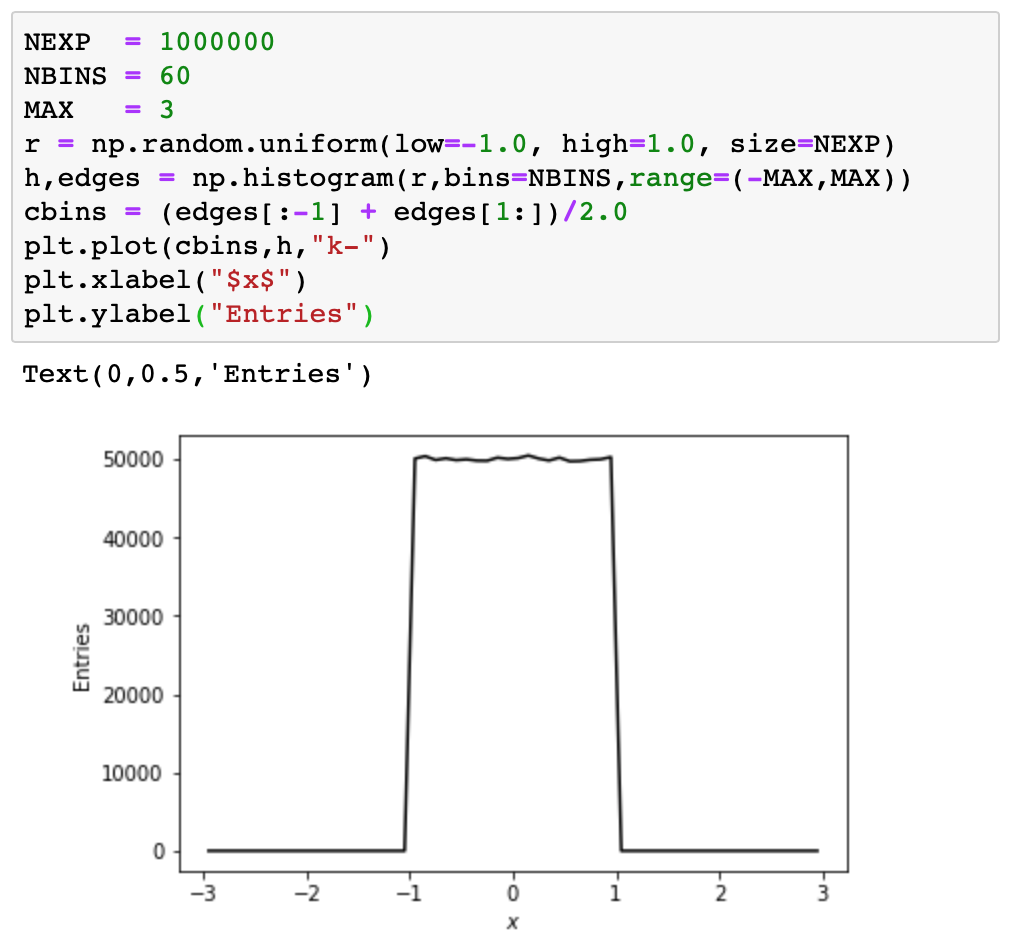
\includegraphics[width=0.75\textwidth]{figs/labs/uncertainties/step.png}\\
\end{center}
\caption{\label{fig:samplingstep} Sampling from the uniform distribution. }
\end{figure}

\begin{figure}[htbp]
\begin{center}
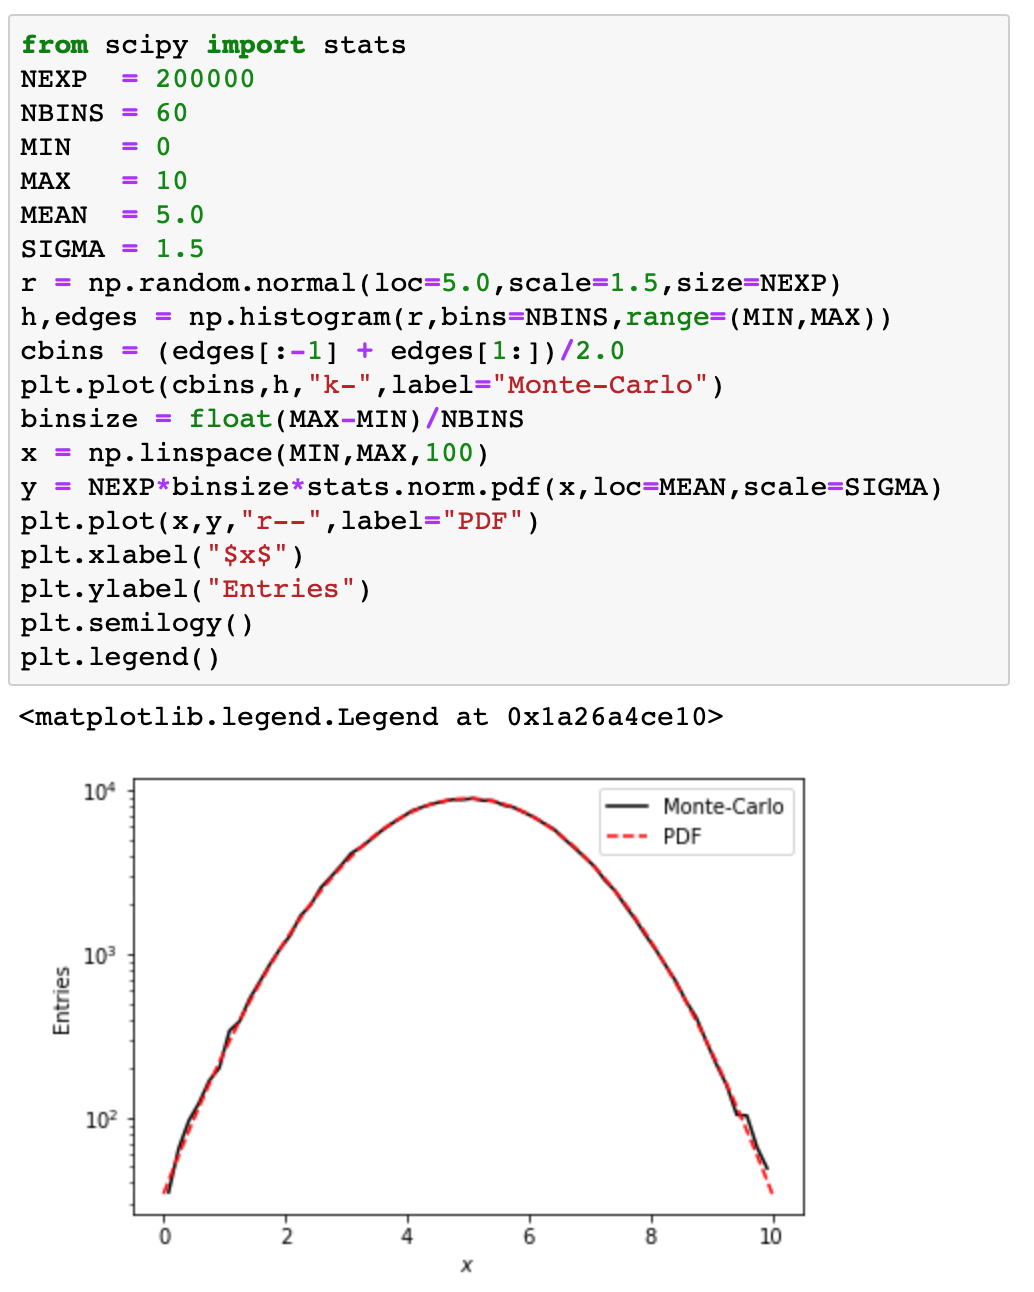
\includegraphics[width=0.75\textwidth]{figs/labs/uncertainties/gaussian.png}\\ 
\end{center}
\caption{\label{fig:samplinggauss} Sampling from the Gaussian distribution and comparison with the Gaussian PDF.}
\end{figure}

Scientific python provides functions to draw random samples according
to various distributions.  In today's lab, we will draw samples
uniformly in the interval $[-1,1]$, as demonstrated in Fig.~\ref{fig:samplingstep}.   The line
\begin{verbatim}
r = np.random.uniform(low=-1.0, high=1.0, size=NEXP)
\end{verbatim}
creates a NumPy array {\tt r} which contains {\tt NEXP} entries, with
each entry chosen uniformly and randomly in the range from -1 to 1.
In the example, these events are displayed in a histogram.  When
plotting histograms with plenty of statistics (one million entries
here) and fine binning (60 bins here) it is usually preferable to use
lines instead of points with error bars for plotting the histograms,
as is done in this example.  Notice, however, that even with one
million events, there are still statistical fluctuations which prevent
the curve from being perfectly smooth.

In Fig.~\ref{fig:samplinggauss}, entries are instead drawn from the Gaussian distribution with the line:
\begin{verbatim}
r = np.random.normal(loc=5.0,scale=1.5,size=NEXP).
\end{verbatim}
The histogram is plotted with a logarithmic $y$ scale:
\begin{verbatim}
plt.semilogy()
\end{verbatim}
which results in the Gaussian distribution appearing as a parabola.  The histogram is compared to the Gaussian PDF appropriately normalized:
\begin{verbatim}
x = np.linspace(MIN,MAX,100)
y = NEXP*binsize*stats.norm.pdf(x,loc=MEAN,scale=SIGMA)
\end{verbatim}


\section{Demonstration of the Central Limit Theorem}

In this section, you'll show that average value of random variables
chosen uniformly from -1 to 1 approaches a Gaussian distribution,
consistent with the central limit theorem.  First create a 2-D array
of size {\tt NEXP} by {\tt NAVG} filled with uniform random values in
the interval from -1 to 1, as follows:
\begin{verbatim}
r = np.random.uniform(low=-1.0, high=1.0, size=(NEXP,NAVG))
\end{verbatim}
Then calculate averages values from {\tt NAVG} entries:
\begin{verbatim}
x = np.sum(r, axis=1)/float(NAVG)  
\end{verbatim}
From the Central Limit Theorem, we expect the entries in x to approach a Gaussian distribution.

\begin{plot}  Set {\tt NEXP} to 1000000 for plenty of statistics.
Produce three different histograms with 40 bins covering the range
from -1.2 to 1.2 for three values {\tt NAVG}: 1,2, and 3.  Plot all
three histogram in the same graph with appropriate legend. \end{plot}

Your plot will show that already for three contributions to the average, the result looks quite Gaussian on a linear scale.  For more precise comparison, will use a log scale and compare to the PDF.

\begin{plot} Calculate {\tt NEXP}$=1000000$ average values {\tt x} for {\tt NAVG}$=10$.  Calculate the mean value of the entries in {\tt x} using the {\tt np.mean} function.  Calculate $\sigma$ for the entries in $x$ by taking the square root of the output from the {\tt np.var} (variance) function.  Produce a histograms with 20 bins covering the range
from -0.5 to 0.5 for the average values.  Compare with a Gaussian distribution, appropriately normalized, using your calculated values from the  mean and sigma.  Plot both the histogram and PDF on the same graph, including an appropriate legend.  Use a logarithmic $y$ axis. \end{plot}


\section{Propagation of Uncertainties}

\begin{figure}[htbp]
\begin{center}
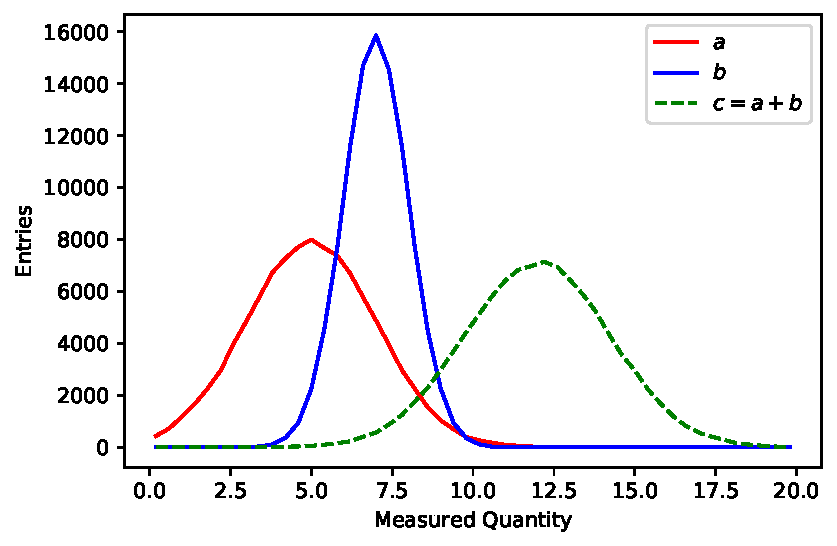
\includegraphics[width=0.75\textwidth]{figs/labs/uncertainties/addunc.pdf}\\
\end{center}
\caption{\label{fig:addunc} Simulation of many measurements of the quantity $c = a + b$. }
\end{figure}

Consider two measured values $a \pm \sigma_a$ and $b \pm \sigma_b$.  If we calculate the quantity $c = a + b$ or $c = a - b$, the uncertainty on the calculated value $c$ is given by:
\begin{displaymath}
\sigma_c = \sqrt{\sigma_a^2 + \sigma_b^2}.
\end{displaymath}
If instead, we calculate $c = a * b$ or $c = a/b$ the fractional uncertainty on $c$ is given by:
\begin{displaymath}
\frac{\sigma_c}{c} = \sqrt{\left(\frac{\sigma_a}{a}\right)^2 + \left(\frac{\sigma_b}{b}\right)^2}.
\end{displaymath}
In this section, you'll develop a numerical simulation for the
propagation of uncertainties under addition, subtraction,
multiplication, and division.  An example, for $c = a + b$ is shown in Fig.~\ref{fig:addunc}.

\begin{print} Pick values for $a$, $b$, $ \sigma_a$ and $ \sigma_b$ for simulating subtraction: $c=a-b$. Print them out in your notebook. Choose the values that are different from what is plotted in Fig.~\ref{fig:addunc}.  \end{print}

\begin{plot} 
Simulate the measurement $a$ by drawing 100,000 random variables
sampled from the Gaussian distribution with mean $a$ and sigma
$\sigma_a$, and likewise for $b$.  Calculate the values of $c = a -b $ from
the $a$ and $b$ values.  Plot the result in histogram with 50 bins and an appropriate range. \end{plot} 

\begin{print} 
Calculate the mean and variance of the mean and variance of the simulated $c$ values and compare to your expectations for the mean, variance of the distribution and variance of the mean. Apply the standard propagation of uncertainties for calculating expectation value for the variances. 
 \end{print}


This is a \textbf{sign-off point} for this lab. 

\begin{print} Pick values for $a$, $b$, $ \sigma_a$ and $ \sigma_b$ for simulating division: $c=a/b$. Print them out in your notebook.  Choose the values that are different from what is plotted in Fig.~\ref{fig:addunc}.  \end{print}

\begin{plot} 
Simulate the measurement $a$ by drawing 100,000 random variables
sampled from the Gaussian distribution with mean $a$ and sigma
$\sigma_a$, and likewise for $b$.  Calculate the values of $c = a/b $ from
the $a$ and $b$ values.  Plot the result in histogram with 50 bins and an appropriate range. \end{plot} 

\begin{print} 
Calculate the mean and variance of the mean and variance of the simulated $c$ values and compare to your expectations for the mean, variance of the distribution and variance of the mean. Apply the standard propagation of uncertainties for calculating expectation value for the variances. 
 \end{print}

 
%{\bf Plot 3-6:}  Produce four plots simulating addition, subtraction, multiplication, and division, as in Fig.~\ref{fig:addunc}.  In each case, compare the measured variance of the $c$ values with your expectation.































\chapter{Curve Fitting}
%ADD CHI2 calculation 
\section{Introduction}

In this lab, you will learn about curve fitting with Scientific Python
function {\tt curve{\_}fit}.  For this lab there are only jupyter notebook entries. 

Given a function to fit $f(x;p)$, with p
representing any number of parameters, and a set of measurements $y_i$ and points $x_i$,
the {\tt curve{\_}fit} function determines the best fit parameters by
minimizing:
\begin{equation}
\chi^2 = \sum_i \frac{(f(x_i;p) - y_i) ^2}{\sigma_i^2}.
\label{eqn:chi2}
\end{equation}
If the uncertainties $\sigma_i$ are not specified, the function
assumes $\sigma_i = 1$, and still finds the correct minimum
if the actual uncertainties are identical to one another.

\section{Fitting a Straight Line}

\begin{figure}[htbp]
\begin{center}
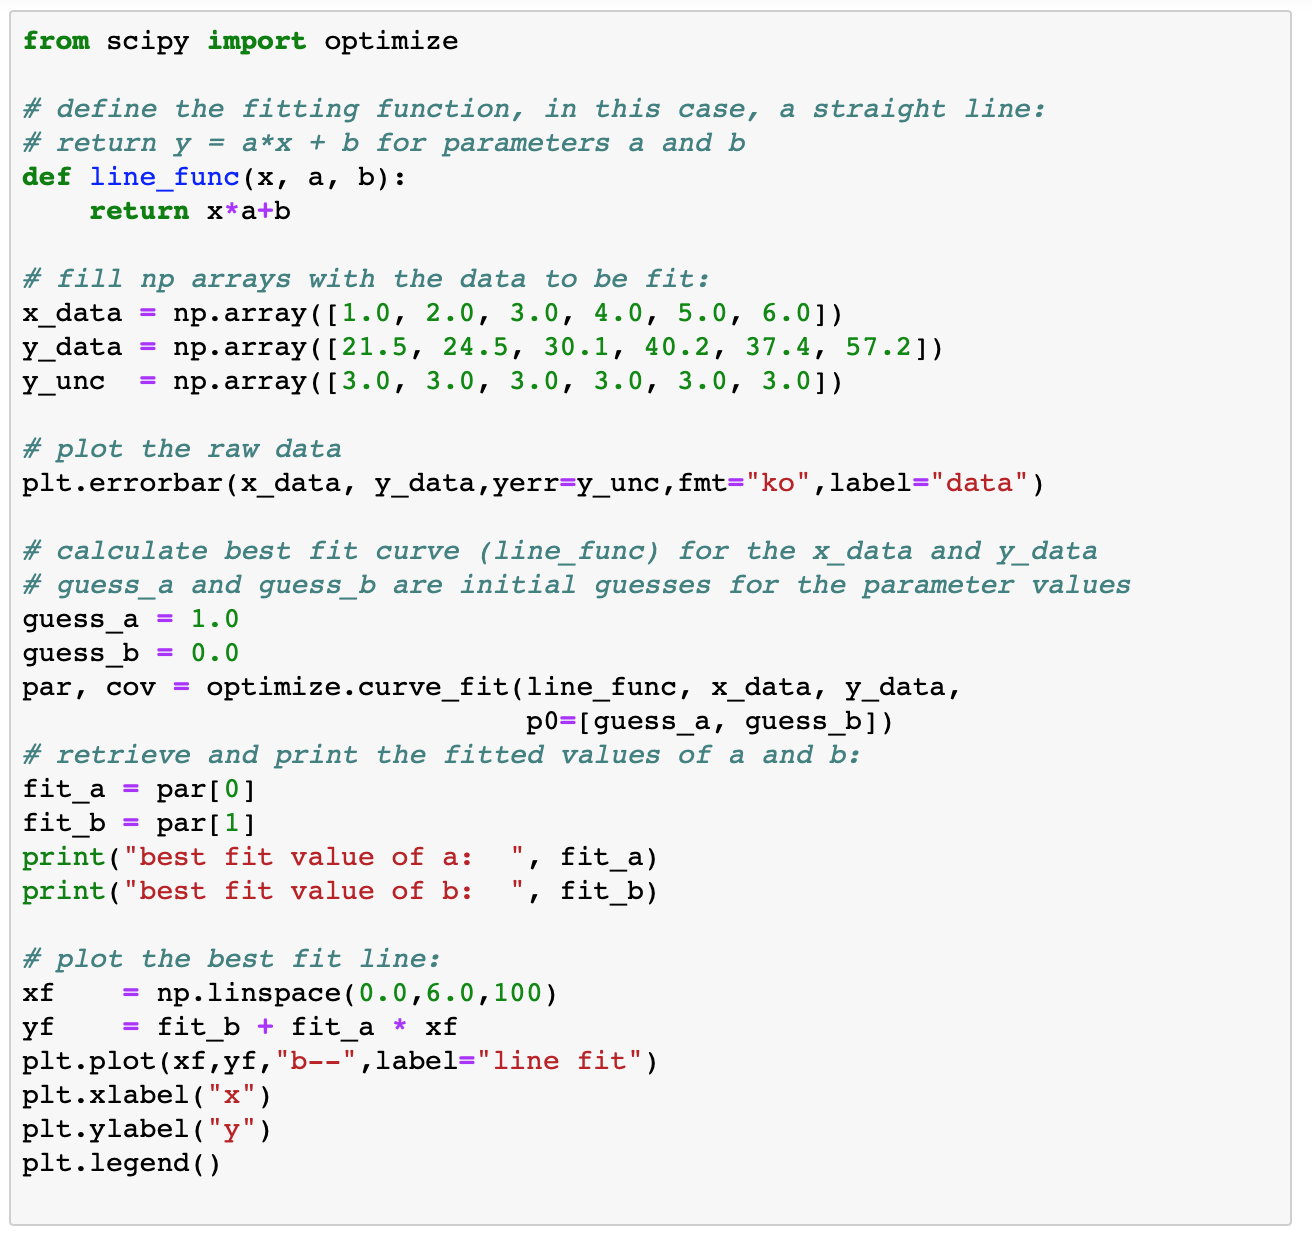
\includegraphics[width=0.65\textwidth]{figs/labs/fitting/fit_code.png} \\
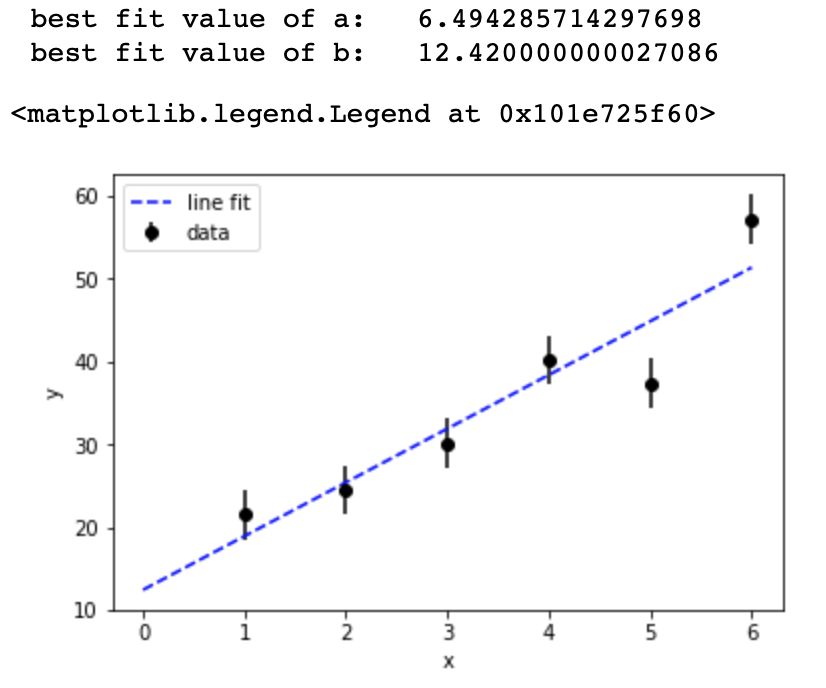
\includegraphics[width=0.65\textwidth]{figs/labs/fitting/fit_out.png} \\
\caption{Example fitting data to straight line.}
\label{fig:fiteg}
\end{center}
\end{figure}

An example using Scientific Pythons {\tt curve{\_}fit} function to fit
a straight line to data is shown in Fig.~\ref{fig:fiteg}.  A block of 
code defining the function we wish to fit, in this case, a straight
line, is defined as a function:
\begin{verbatim}
     def line_func(x, a, b):
         return a*x + b
\end{verbatim}
In this case, the function requires three parameters (in the computer
science sense) the x data in a numpy array as function parameter x,
the slope as function parameter a, and the intercept as function
parameter b.  When called, the function returns the x data multiplied
by the value a, with the value b added.  We don't directly call this
function, but in principle, it could be called like:
\begin{verbatim}
    y_data = line_func(x_data, 2.0, 0.0)
\end{verbatim}
to create a numpy array {\tt y{\_}data} constructed from {\tt
  x{\_}data} with slope 2 and intercept 0.

The next section filling numpy arrays containing the data, and
plotting it with error bars should be familiar by now.  The fit itself
is performed by the line:
\begin{verbatim}
par, cov = optimize.curve_fit(line_func, x_data, y_data, p0=[guess_a, guess_b])
\end{verbatim}
This performs a fit of the function {\tt line{\_}func} defined above
to the $x$ and $y$ data contained in the arrays {\tt x{\_}data} and
{\tt y{\_}data}.  Numerical fits generally find the local minimum,
which is not necessarily the global minimum of interest.  It is
important therefore, especially for complicated fits, to provide an
initial guess near the expected fit values.  These are provided to the
optional, named, function parameter {\tt p0}, which is set to the
python list {\tt [guess{\_}a, guess{\_}b]} which contains our initial guesses for
the fit parameters $a$ and $b$.  The function performs a least-squares
fit to find the best values of $a$ and $b$ which are returned as the
numpy array {\tt par}.  The function also returns the covariance
matrix as the numpy array {\tt cov}.

The remaining code simply uses the best fit values to plot the fitted
function as a dashed line.  Numerical fits are fickle.  Even if you
are only interested in the fitted value, you should always plot the
best-fit function and compare the results to your data as in important
check for your work.

\begin{table}
\caption{Sample data for straight line fit.}
\label{tbl:linesamp}
\begin{center}
\begin{tabular}{ll}
$x$ & $y \pm \sigma_y$ \\
1.0  & $15.9 \pm 3.0$ \\
2.0  & $23.6 \pm 3.0$ \\
3.0  & $33.9 \pm 3.0$ \\
4.0  & $39.7 \pm 3.0$ \\
5.0  & $45.0 \pm 10.0$ \\
6.0  & $32.4 \pm 20.0$ \\
\end{tabular}
\end{center}
\end{table}

%\begin{figure}[htbp]
%\begin{center}
%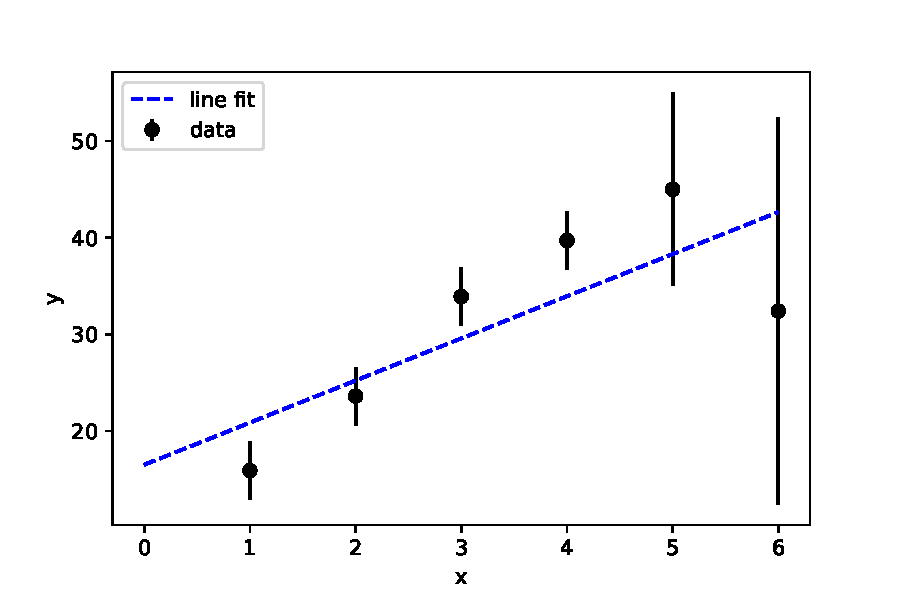
\includegraphics[width=0.65\textwidth]{figs/labs/fitting/bias.pdf} 
%\caption{This linear fit is biased by the failure to properly account for uncertainties.}
%\label{fig:fitbias}
%\end{center}
%\end{figure}

\begin{plot} Apply a code like that of Fig.~\ref{fig:fiteg}
to the data in Table~\ref{tbl:linesamp}. Plot the data including error bars and the best-fit function.
% reproduce the plot in Fig.~\ref{fig:fitbias}.  
\end{plot}

Notice that the last two data points have larger uncertainties than
the other data points.  However, the call to the {curve{\_}fit}
function does not provide the parameter uncertainties, and so the
function assumes that they all have the value $1$.  In this case,
since the uncertainties are not in fact all the same, the function
does not find the correct minimum.  The answer is clearly biased
toward the poorly measured points, because the function gives these
points the same weight as all of the other points.

\begin{print} The {\tt curve{\_}fit} function does not provide directly the $\chi^2$ value of the fit. However you can calculate it manually via equation~\ref{eqn:chi2}. The sum can be obtained via numpy function sum. Modify your code to include calculation of the $\chi^2$ value of the fit. Include also the calculation of the $\chi^2$ divided by the number of degrees of freedom (number of data points minus number of parameters), which is called reduced $\chi^2$. Print both of those values. Is the fit reasonable based on the reduced $\chi^2$ value? Print your comment as well. 
\end{print}

\begin{plot} Look-up the {\tt curve{\_}fit} function and the optional parameter
{\tt sigma}. Provide the correct uncertainties to
the fit and make a new plot with the data and the fit.  You should observe that the fit results is no longer biased,
and more closely tracks the well constrained left side of the plot. \end{plot}

\begin{print} Print $\chi^2$ and reduced $\chi^2$ value. Is the fit reasonable based on the reduced $\chi^2$ value? Print your comment as well. \end{print}

\section{Parameter Uncertainties I}
\label{sec:sigmatrue}
As discussed in the lecture the uncertainty $\sigma_{p_i}$ on the $i$th parameter $p_i$
can be determined from the second derivative of the $\chi^2$ function:
\begin{displaymath}
\frac{d^2\chi^2}{d p_i^2} = \frac{2}{\sigma_{p_i}^2}.
\end{displaymath}
In general, for $M$ parameters, the $M \times M$ covariance matrix is calculated as:
\begin{displaymath}
C(i,j) = 2 \cdot \left(\dfrac{d^2\chi^2}{d p_i d p_j} \right)^{-1}
\end{displaymath}
from which we can see that the diagonals are simply the parameter uncertainties squared:
\begin{displaymath}
C(i,i) = 2 \cdot \left(\dfrac{d^2\chi^2}{d p_i^2} \right)^{-1} = \sigma^2_{p_i}.
\end{displaymath}
The off-diagonal elements contain information about how parameters are
correlated, and for a well designed fit function they should be close to
zero.

The {\tt curve{\_}fit} function returns both the best fit parameter values and the covariance matrix:
\begin{verbatim}
par, cov = optimize.curve_fit(...)
\end{verbatim}
For a fit with $M$ parameters, we can obtain an array containing the
$M$ parameter uncertainties from the square root of the diagonals of the $M \times M$
covariance matrix:
\begin{verbatim}
unc = np.sqrt(np.diag(cov))
\end{verbatim}

We can obtain uncertainties of parameters by accessing elements of the array.

Lets study this in an example for $N=1$ parameter. Generate $x$-values as a numpy array of evenly spaced values from 0 to 99. Generate $y$-values as 100 random numbers drawn from a Gaussian distribution with mean $m = 50$ and a width $\sigma_y =10$.  Perform a fit using {\tt curve{\_}fit} function. Set the uncertainties on the $y$ values to 10 and also set parameter {\tt absolute{\_}sigma = True}.  

 The best fit constant value we expect is simply the mean of the $y$-values.  The
uncertainty on the mean value should be:
\begin{displaymath}
\sigma_m = \sigma_y / \sqrt{N} = 10 / \sqrt{100} = 1.0
\end{displaymath}

\begin{print} Calculate the expected values for the best fit value and its uncertainty. Print them together with the fitted best fit value and its uncertainty. Do those agree? \end{print}


\section{Fitting a Sine Curve}

In this section, you will fit the sample data to a sine function:
\begin{displaymath}
 y = A \, \sin( k x). 
\end{displaymath}
Use the following sample data:\\
\begin{center}
\begin{tabular}{|ll| ll|ll|}
\hline
$x$ & $y$ & $x$ & $y$ & $x$ & $y$\\
\hline
0  & 5.3    & 4  & -9.7   & 8  & 15.7  \\
1  & 15.0   & 5  & -17.4  & 9  & 18.5  \\
2  & 19.2   & 6  & -20.5  & 10 & 8.6   \\
3  & 6.8    & 7  &  2.1   & &  \\
\hline
\end{tabular}
\end{center}
Assume the uncertainty is the same for each $y$ value: $\sigma_i = 2$.
\begin{plot} Plot the data including error bars and the best-fit
sine wave. \end{plot}

\begin{print} Print the best fit parameter
values and their uncertainties. \end{print}

Remember to set {\tt absolute{\_}sigma=True}.\\

This is a \textbf{sign-off point} for this lab. 

\section{Parameter Uncertainties II}

%\begin{figure}[htbp]
%\begin{center}
%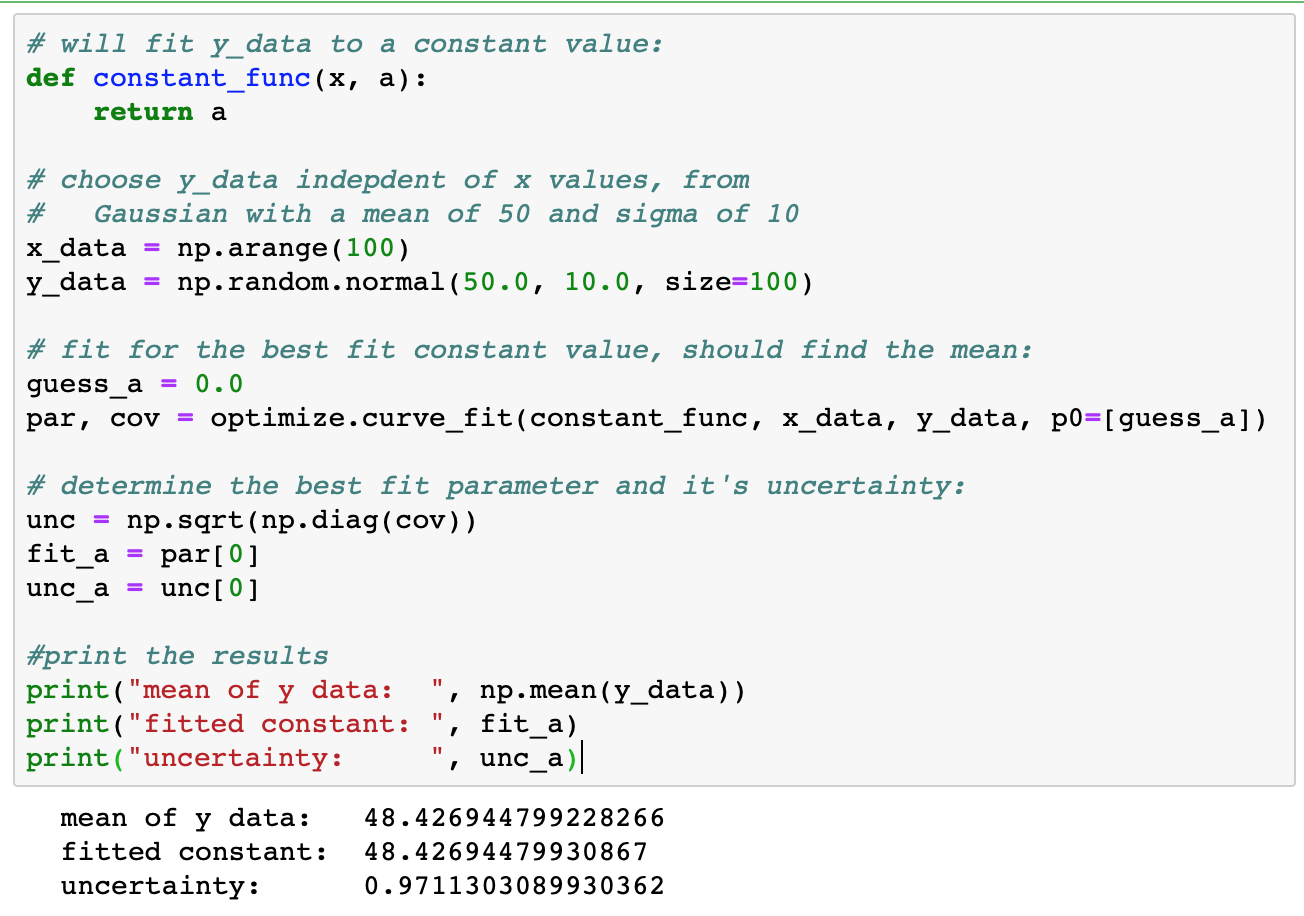
\includegraphics[width=0.65\textwidth]{figs/labs/fitting/uncertainties.png} \\
%\caption{Example obtaining parameter uncertainties.}
%\label{fig:fitunc}
%\end{center}
%\end{figure}

Lets repeat the study in~\ref{sec:sigmatrue}. Generate $x$-values as a numpy array of evenly spaced values from 0 to 99. Generate $y$-values as 100 random numbers drawn from a Gaussian distribution with mean $m = 50$ and a width $\sigma_y =10$.  Perform a fit using {\tt curve{\_}fit} function.  Leave the uncertainties on the $y$ values
unspecified and also leave parameter {\tt absolute{\_}sigma} unspecified. 

\begin{print} Print the fitted best fit value and its uncertainty. \end{print}

It's surprising actually, that the fit returns the correct
uncertainty.  Your code does not provide  the uncertainty on the $y$ parameters $\sigma_y$ to
the fit.  So how can it possible deduce the correct uncertainty
$\sigma_m = \sigma_y / \sqrt{N}$?

The answer is that behind the scenes, the {\tt curve{\_}fit} function
is being really quite clever (too clever, in my opinion, for a default
behavior!)  By default, the covariance matrix returned by the 
{\tt curve{\_}fit} function is scaled by the factor:
\begin{displaymath}
\alpha = \frac{\chi^2_{\rm min}}{\rm NDF}
\end{displaymath}
the minimum value of the $\chi^2$ divided by the number of degrees of
freedom (number of data points minus number of parameters).  As discussed in lecture that $\alpha$ is around 1 for a least-squares fit with
an appropriate model and correct uncertainties.  So nominally this
factor is one, and has no effect.  But consider what happens if the
actual uncertainties are $\sigma$ while the $\chi^2$ used in the fit assumes they
are, for example, ``1''.  In this case, the calculated $\chi^2$ is:
\begin{displaymath}
\chi^2 = \sum_i \frac{(f(x_i;p) - y_i) ^2}{1}
\end{displaymath}
which differs from the correct $\chi^2$:
\begin{displaymath}
\chi^2 = \sum_i \frac{(f(x_i;p) - y_i) ^2}{\sigma^2}
\end{displaymath}
by a factor of $\sigma^2$.  This means that while the correct value
for $\alpha$ is nearly one, the calculated value of alpha will be
$\sigma^2$.  This is precisely the factor needed to scale the squared
parameter uncertainties to account for the fact that the initial
uncertainty was $\sigma$ but we assumed $1$.

This behavior is controlled by the parameter {\tt absolute{\_}sigma}.
By default, the function sets {\tt absolute{\_}sigma = False} and
scales the covariance matrix as just described.  On the other hand, if
you want to simply use the provided uncertainties without re-scaling
the covariance matrix, you must remember to set {\tt
  absolute{\_}sigma = True}.  I think this is a really poor choice of
default behavior...  it's really quite a fancy thing to do implicitly.
In cases when you know the uncertainty on your data points, this
re-scaling actually results in less correct estimate for the
uncertainties.  This is because for a good model with proper
uncertainties, the factor $\alpha$ is near one, but not exactly one.

\begin{print} Repeat the study but leave the uncertainties on the $y$ values
unspecified and set {\tt absolute{\_}sigma = True} in the fit.  You
should obtain an uncertainty of $0.1$.  Print your value and print your explanation of
why you obtained this value. \end{print}

As a rule of thumb, when using {\tt curve{\_}fit}, if you provide
explicit uncertainties, you should remember to set {\tt
  absolute{\_}sigma = True}.  And really, for precision work, you should
almost always be providing explicit uncertainties.



















\chapter{Simulation of an Ideal Gas}

\section{Introduction}

For an ideal gas composed of molecules with mass $m$ at temperature
$T$, the probability density for the component of velocity in the $x$
direction ($v_x$) is given by:
\begin{equation}
  \label{eqn:mbvx}
P(v_x) = \sqrt{\frac{m}{2 \pi k_{\rm B} T}} \exp\left(-\frac{m v_x^2}{2k_{\rm B} T}\right)
\end{equation}
where $k_{\rm B}$ is Boltzmann's constant.  Similary for the $y$ direction:
\begin{equation}
  \label{eqn:mbvx}
P(v_y) = \sqrt{\frac{m}{2 \pi k_{\rm B} T}} \exp\left(-\frac{m v_y^2}{2k_{\rm B} T}\right).
\end{equation}

For simplicity, we will be simulating a gas in two dimensions.  The infinitesimal probability associated with a velocity $(v_x, v_y)$ is given by: 
\begin{eqnarray*}
P(v_x, v_y) \, dv_x \, dv_y &=& P(v_x) \, dv_x \, P(v_y) \, dv_y \\
   &=& \frac{m}{2 \pi k_{\rm B} T} \exp\left(-\frac{m (v_x^2+v_y^2)}{2k_{\rm B} T}\right) \, dv_x \, dv_y \\
   &=& \frac{m v}{2 \pi k_{\rm B} T} \exp\left(-\frac{m v^2}{2k_{\rm B} T}\right) \, d\theta \, dv \\
\end{eqnarray*}
where we have changed to polar coordinates $v$ and $\theta$ in the usual manner with area differential $dv_x \, dv_y = v \, dv \, d\theta$.  This allows us to read off the probability density in polar coordintes:
\begin{equation*}
P(v, \theta) = \frac{m v}{2 \pi k_{\rm B} T} \exp\left(-\frac{m v^2}{2k_{\rm B} T}\right) 
\end{equation*}
Integrating over all possible directions $\theta$, we obtain:
\begin{eqnarray}
P(v) &=& \int_0^{2\pi} P(v,\theta) d\theta \nonumber \\
     &=& \int_0^{2\pi} \frac{m v}{2 \pi k_{\rm B} T} \exp\left(-\frac{m v^2}{2k_{\rm B} T}\right) \nonumber \\
P(v) &=& \frac{m v}{k_{\rm B} T} \exp \left(-\frac{m v^2}{2k_{\rm B} T}\right) \label{eqn:mbv}\\
\nonumber
\end{eqnarray}
which is the Maxwell-Boltzmann distribution for an ideal gas in two
dimensions.  This is the probability density for a gas molecule to have speed
$v$.

In this lab, we will create a simple numerical simulation of an ideal
gas and verify that the velocity of the gas follows the
Maxwell-Boltzmann distribution.

\section{System of Units}

Choosing an effective system of units is essential for building a
well-behaved numerical simulation.  Consider the Maxwell-Boltzmann
distribution, which involves the following SI values:
\begin{itemize}
\item Boltzmann's constant: $k_{\rm B} = 1.38 \times 10^{-23}~\rm J/K$
\item Molecular masses: e.g. $N_2$ with $m =  4.65 \times 10^{-26}~ \rm kg$.
\item Temperature: e.g. room temperature $T = 293~\rm K$.
\end{itemize}
The smallest number greater than zero that a computer can represent
with a single-precision floating point number is approximately
$10^{-38}$. Representing the SI value of Boltzmann's constant at
$10^{-23}$ uses a large fraction of this precision before we even begin
our calculation.  Numerical algorithms using floating point numbers
work best when the values involved in the calculation are near one.

It is usually best, therefore, to devise an alternate system of units
for any numerical simulation which keeps the values of variables of
interest as near one as possible.  We will call this the numerical
system of units.

To start, we choose a reference temperature near the temperature
we would like to simluate, say $T_0 = 293~\rm K$.  All temperatures in
the simulation will be in units of this reference temperature.  So a
temperature {\tt T=1.2} in the program will be $1.2 \, T_0 = 352~\rm K$
in SI units.  Our model also includes mass, so we choose a reference
mass near the mass of the molecules we will be simulating, say $M_0 =
4.65 \times 10^{-26}~ \rm kg$.  A mass {\tt m=2.1} in our program would have
an SI value value of $2.1 M_0 = 9.8 \times 10^{-26}~ \rm kg$.

The physics we will simulate involves Boltzmann's constant $k_{\rm B}$
which will have a value of one in our program.  This sets the
reference energy from our reference temeperature.  For example, an
energy {\tt kT = 3} in our program will have an SI value of $k_{\rm B}
T = 3~k_B T_0 = 1.21 \times 10^{-20}~J$.  The reference energy and
reference mass together define a reference velocity:
\begin{displaymath}
V_0 = \sqrt{\frac{k_b T_0}{M_0}} = 295~ \rm m/s.  
\end{displaymath}  

The only time the actual values choosen for the numerical system of
units are needed is if you need to convert inputs in SI units to the
numerical system of units, or convert the results of your simulation
to SI units.  In this lab, we will specify all inputs and report all
results using the numerical system of units.  {\bf So there is no need for
specific values such as $M_0 = 2.32 \times 10^{-25}~\rm kg$ to appear
anywhere in your program.}  If such values do appear, outside of
comments, you are certainly making a mistake!

\begin{figure}[htbp]
\begin{center}
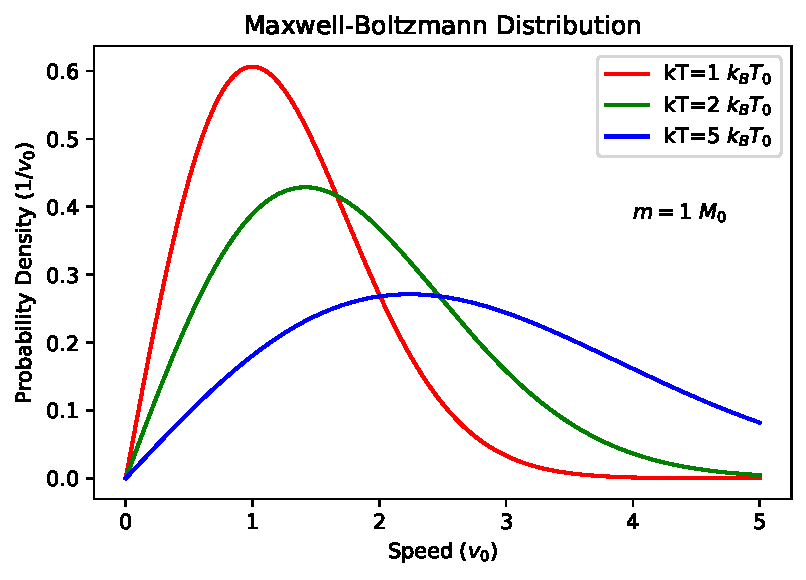
\includegraphics[width=0.65\textwidth]{figs/maxwellboltzman/maxboltz.pdf} \\
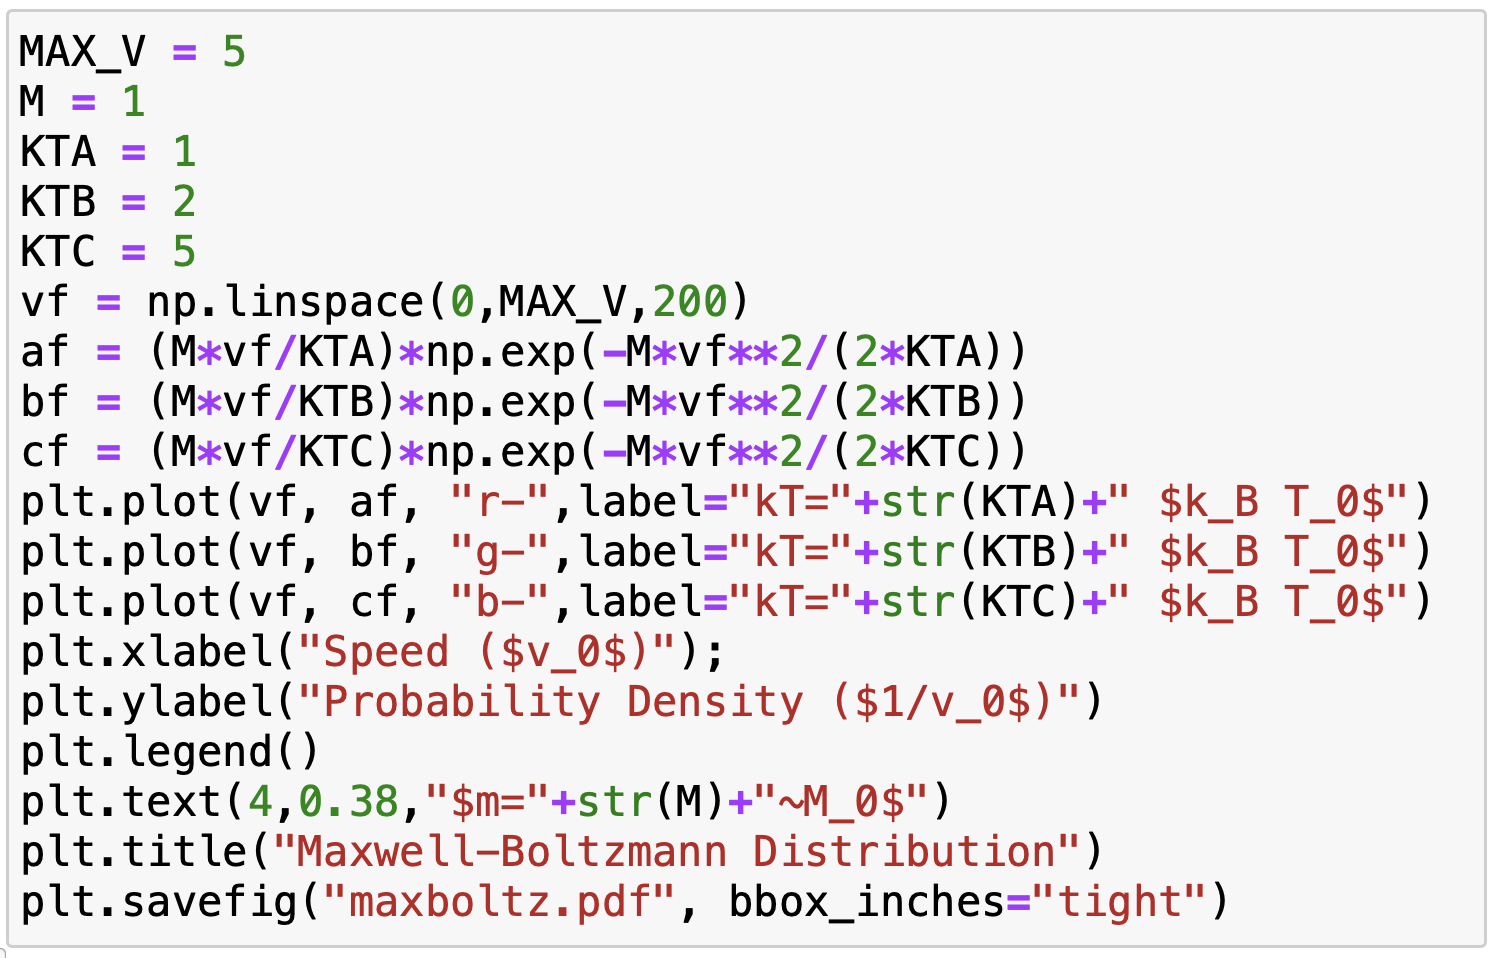
\includegraphics[width=0.65\textwidth]{figs/maxwellboltzman/maxboltz-code.png} \\
\caption{The Maxwell-Boltzmann distribution using a system of units appropriate for a numerical simulation, along with the code used to produce the plot.}
\label{fig:mbdist}
\end{center}
\end{figure}

As an example, the Maxwell-Boltzmann distribution is plotted in
Fig.~\ref{fig:mbdist} alongside the code used to produce it.  Notice
how for {\tt kT} and {\tt m} near one, the typical velcities are also
near one.  This is sign of good numerical system of units.  Notice
also that Boltzmann's constant or any other small or large numbers in
SI units do not appear anywhere in the code. 

\section{Collision Model}

At the heart of your numerical simulation is the collision model.  It
is the collisions of molecules that will allow your simulated gas to
reach thermal equilibrium.  We will use the simple elastic collision
of identical mass particles, as illustrated in Fig.~\ref{fig:collcms}, as our collision model.  We consider particles a and b with velocities $\vec{v_a}$ and
$\vec{v_b}$ in the lab frame.  The velocity of particle a in the CMS frame before the collision is
\begin{displaymath}
\vec{u} = \frac{\vec{v_a} - \vec{v_b}}{2}.
\end{displaymath}
The collision rotates the velocity of particle a by the scattering angle $\theta$ so that the velocity $\vec{w}$ after the collision is
\begin{displaymath}
\begin{pmatrix}
w_x \\
w_y \\
\end{pmatrix}
  =
\begin{pmatrix}
\cos \theta  & \sin \theta \\
-\sin \theta  & \cos \theta \\
\end{pmatrix}
\,
\begin{pmatrix}
u_x \\
u_y \\
\end{pmatrix}
\end{displaymath}
In the lab frame, the velocity of molecule a changes by an amount:
\begin{displaymath}
\Delta \vec{v_a} = \vec{w} - \vec{u}
\end{displaymath}
and the velocity of molecule b changes by an amount:
\begin{displaymath}
\Delta \vec{v_b} = \vec{u} - \vec{w}
\end{displaymath}




\begin{figure}[htbp]
\begin{center}
\begin{tikzpicture}
\draw[->, line width=1.5, blue] (-3,0) -- (-0.1,0);
\draw[->, line width=1.5, blue] (3,0)  -- (0.1,0);
\draw[->, line width=1.5, red] (0,0) -- (3*0.50,3*0.86) coordinate(A);
\draw[->, line width=1.5, red] (0,0) -- (-3*0.50,-3*0.86) coordinate(B);
\node[right] at (0.5,0.5) {$\theta$};
\node[left] at (-3,0) {a};
\node[right] at (3,0) {b};
\node[above] at (A) {a};
\node[below] at (B) {b};
\node[above] at (-1.5,0) {$\vec{u}$};
\node[above] at (1.5,0) {$-\vec{u}$};
\node[left] at (0.8,1.5) {$\vec{w}$};
\node[left] at (-0.8,-1.4) {$-\vec{w}$};
\end{tikzpicture}
\caption{The collision model in the center-of-mass:  incoming molecule $a$ with velocity $\vec{u}$ collides with the incoming particle $b$ of identical mass with velocity $-\vec{u}$.  Particle $a$ is scattered by angle $\theta$ and leaves with velocity $\vec{w}$, while particle $b$ leaves with velocity $\vec{w}$.  The magnitude of the final and initial velocities are the same:  $|\vec{u}| = |\vec{w}|$.}
\label{fig:collcms}
\end{center}
\end{figure}

\section{Implementing the Collision Model}

Our Python implementation for the collision will be computed in terms
of the components of the velocity vectors of molecule a and molecule
b:
\begin{eqnarray*}
\vec{v_a} &=& 
\begin{pmatrix}
a_x \\
a_y \\
\end{pmatrix} \\
\vec{v_b} &=& 
\begin{pmatrix}
b_x \\
b_y \\
\end{pmatrix} \\
\end{eqnarray*}
We'll use the Python variable names {\tt ax}, {\tt ay}, {\tt bx}, and {\tt by} to refer to $a_x$,  $a_y$,  $b_x$, and $b_y$.  

First calculate the $x$ and $y$ component of $\vec{u}$ as:
\begin{eqnarray*}
u_x &\equiv& \frac{a_x - b_x}{2} \\
u_y &\equiv& \frac{a_y - b_y}{2} \\
\end{eqnarray*}
Then compute the $x$ and $y$ component to the change in velocity of particle a and particle b:
\begin{eqnarray*}
  \Delta a_x &=& (\cos\theta - 1) \, u_x + \sin\theta \, u_y \\
  \Delta a_y &=& (\cos\theta - 1) \, u_y - \sin\theta \,  u_x \\
  \Delta b_x &=& (1-\cos\theta) \, u_x - \sin\theta \, u_y \\
  \Delta b_y &=& (1-\cos\theta) \, u_y + \sin\theta \,  u_x \\
\end{eqnarray*}
Finally, update the $x$ and $y$ components of the particle velocities to their value after the collision:
\begin{eqnarray*}
  a_x &\to& a_x + \Delta a_x \\
  a_y &\to& a_y + \Delta a_y \\
  b_x &\to& b_x + \Delta b_x \\
  b_y &\to& b_y + \Delta b_y \\
\end{eqnarray*}

In essential technique for programming complicated task is dividing
complicated tasks into smaller tasks, and thoroughly testing the
smaller tasks.  You cannot program effectively until you master this
technique.  I've taught students programming for many years, and the
students that finish last are invariably the ones that rush to
complete their entire program and then try to test and debug it.  This
approach always fails because when you do not get the right answer,
and you won't, ever, on the first try, you have absolutely no idea
what part of a very long chain of calculations is not programmed
correctly.

\begin{figure}[htbp]
\begin{center}
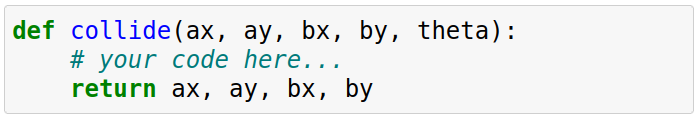
\includegraphics[width=0.65\textwidth]{figs/maxwellboltzman/collide.png} \\
\caption{Collision function.}
\label{fig:collfunc}
\end{center}
\end{figure}


To use this approach in the lab, we'll be implementing the collision
algorithm as a function, exactly as in Fig.~\ref{fig:collfunc}.  This
function takes as input the velocity components {\tt ax}, {\tt ay},
{\tt bx}, {\tt by} as defined above plus the scattering angle {\tt
  theta}.  In Fig.~\ref{fig:collfunc}, the function simply returns the
velocity components unchanged.  You should modify the function to
implement the scattering algoirthm described above.

Normally at this point, you would have to devise your own test to
validate your code.  One technique, that would work here, is to
calculate a few examples and then compare your program output to what
you obtained with paper and pencil.  For this lab, I will provide some
specific example calculations for you to validate your collision function.

\begin{figure}[htbp]
\begin{center}
  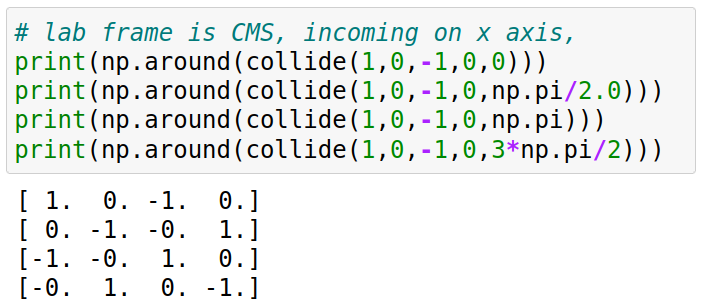
\includegraphics[width=0.65\textwidth]{figs/maxwellboltzman/collx.png} \\
  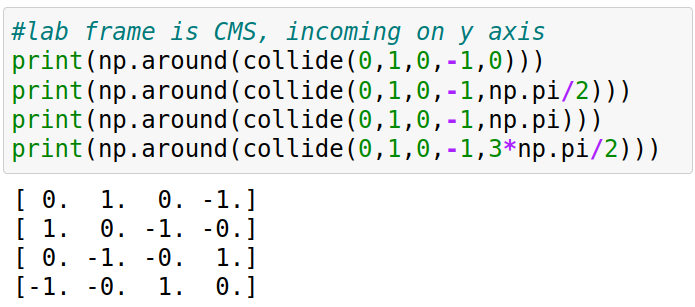
\includegraphics[width=0.65\textwidth]{figs/maxwellboltzman/colly.png} \\
  \caption{Example collisions along the $x$ and $y$ axis.}
\label{fig:collxy}
\end{center}
\end{figure}

\begin{plot} \end{plot}  Implement the collision algorithm as a function as in Fig.~\ref{fig:collfunc} and test it using example collisions from Fig.~\ref{fig:collxy}.

When testing your code, start with easy, special cases, such as used in Fig.~\ref{fig:collfunc}.  This helps makes it clearer where the program is failing.  Once your code works on the simple cases, escalate to more complicated examples.

\begin{figure}[htbp]
\begin{center}
  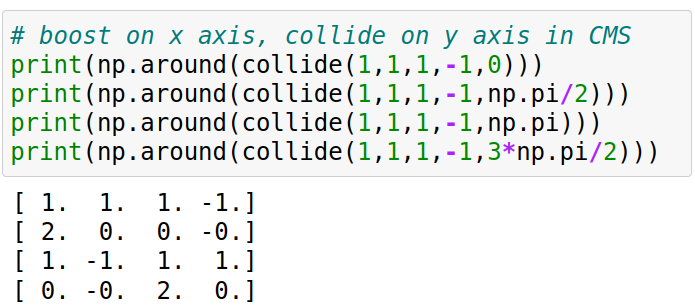
\includegraphics[width=0.65\textwidth]{figs/maxwellboltzman/collxy.png} \\
  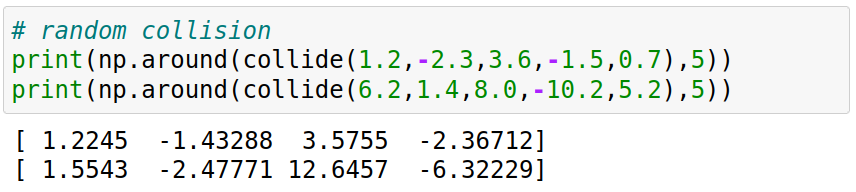
\includegraphics[width=0.65\textwidth]{figs/maxwellboltzman/collrand.png} \\
  \caption{More complicated example collisions.}
\label{fig:collcomp}
\end{center}
\end{figure}

\begin{plot} \end{plot}  Test your collision algorithm using the  example collisions from Fig.~\ref{fig:collcomp}.

\section{Initializing the Simulated Ideal Gas}

You will be modeling an ideal gas by direct Monte Carlo simulation of
{\tt NGAS} representative molecules.  We will use {\tt NGAS=1000}
intially, and you should use an even lower value while debugging.
We'll assume that the mass of each molecule in the gas is $M_0$,
or in the numerical system of units {\tt M=1}.

The state of your simulation will be completely contained in two numpy
arrays {\tt vx} and {\tt vy}, each of length {\tt NGAS}, which contain
the velocities of the particles in units of $V_0 = \sqrt{k_b T_0 /
  M_0}$.  Remember, the simulation uses a system of units that should
keep velocities near 1, so values such as 2.2, -3.1, 0.8, -0.01 are
all likely, and correspond to speeds up to several hundred meters per
second in SI units.  On the other hand, the presence of extremely
small values, like 5.3E-23, and extremely large values like 1.2E18 and
-8.2E28 are symptoms of bugs.

\begin{plot} Initialize both velocity arrays {\tt vx} and {\tt vy} of length {\tt NGAS}
with values choosen as uniform random variables in the range
$[-2,2]$. Fill two histograms, one with $v_x$ and one with $v_y$, with
an approriate range and 20 bins.  You should see that the velocities
are distributed uniformly (a flat distribution).  The distribution does not yet
resemble the Gaussian shape of Equation~\ref{eqn:mbvx} because it has not yet reached
thermal equilibrium.\end{plot}


\section{Collisions of an Ideal Gas}

To reach thermal equilibrium, you'll need to simulate collisions
betweens pairs of molecules in your gas.  For each collision, do the following:
\begin{itemize}
 \item Choose two molecules at random as particles $a$ and $b$. (See {\tt np.random.choice}.)
 \item Choose a random value $\theta$ uniformly in the range $[0,2\pi]$ (See {\tt np.random.uniform}.)
 \item Call your collision function with components of the velocity vectors for particles $a$ and $b$ and the scattering angle $\theta$.
 \item Update the velocity of particles $a$ and $b$ from the return value of your collision funciton
\end{itemize}   
For this model, you will need about 10 times as many collisions as gas
molecules in order to reach thermal equilibrium.

\begin{plot}  For {\tt NGAS=1000} simulate {\tt NCOLL = 10000} collisions as described above.
Fill two histograms, one with $v_x$ and one with $v_y$, with an
approriate range and 20 bins.  After reaching thermal equilibrium, the
distributions should resemble a Gaussian as predicted by Equation~\ref{eqn:mbvx}. \end{plot}

\section{Temperature of an Ideal Gas}

The temperature of the gas is related to the mean kinetic energy by:
\begin{equation}
\label{eqn:kt}
k_b T = m \, \frac{\braket{v_x^2} + \braket{v_y^2}}{2}  
\end{equation}  
You can estimate $\braket{v_x^2}$ from your simulation as {\tt np.mean(vx**2)}.

\begin{plot} Estimate $kT$ of the gas using Equation~\ref{eqn:kt} before and after simulating collisions.
The values should remain near the expected value 4/3.
\end{plot}

\section{The Maxwell-Boltzmann Distribution}

In this section, you'll reproduce the instructor plots of Fig.~\ref{fig:mbinst} using your own numerical simulation.

\begin{figure}[htbp]
\begin{center}
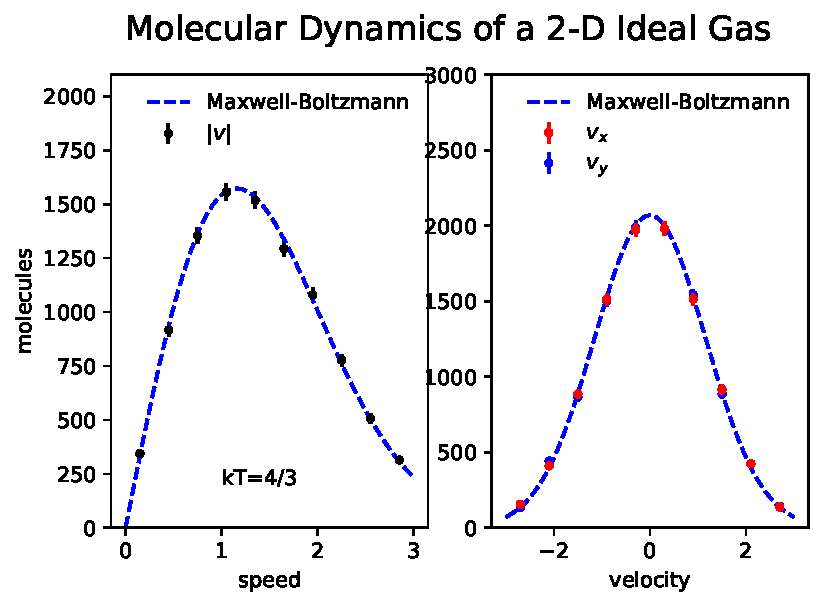
\includegraphics[width=0.85\textwidth]{figs/maxwellboltzman/maxboltz-instr.pdf} \\
\caption{Instructor plots.}
\label{fig:mbinst}
\end{center}
\end{figure}

\begin{plot}
  After your simulation reaches equilibrium, fill two histograms, one with $v_x$ and one with $v_y$, with an approriate range and 10 bins.  Compare with the prediction from Equation~\ref{eqn:mbvx}.  The results should resemble the right side of Fig.~\ref{fig:mbinst}, which were produced with {\tt NGAS=10000}.
\end{plot}

\begin{plot}
  After your simulation reaches equilibrium, fill a histograms with the magnitude of the velocity $v$, with an approriate range and 10 bins.  Compare with the prediction from Equation~\ref{eqn:mbv}.  The results should resemble the left side of Fig.~\ref{fig:mbinst}, which were produced with {\tt NGAS=10000}.
\end{plot}


  


\end{document}



\input{lab_gas.tex}

\chapter{Fourier Series and Transform}

\section{Introduction}

This lab will introduce the Fourier Series and Transform.


%\section{Example Plots} 
%\begin{figure}[htbp]
%\begin{center}
%\includegraphics[width=0.65\textwidth]{figs/labs//plotting/plotting.png} 
%\caption{Sine function sampled at discrete values.}
%\label{fig:plotsin}
%\end{center}
%\end{figure}


\chapter{Simulating a Guitar String}

\section{Introduction}

This lab will introduce the Fourier Series and Transform.


%\section{Example Plots} 
%\begin{figure}[htbp]
%\begin{center}
%\includegraphics[width=0.65\textwidth]{figs/labs//plotting/plotting.png} 
%\caption{Sine function sampled at discrete values.}
%\label{fig:plotsin}
%\end{center}
%\end{figure}



\chapter{Curve Fitting}
%ADD CHI2 calculation 
\section{Introduction}

In this lab, you will learn about curve fitting with Scientific Python
function {\tt curve{\_}fit}.  For this lab there are only jupyter notebook entries. 

Given a function to fit $f(x;p)$, with p
representing any number of parameters, and a set of measurements $y_i$ and points $x_i$,
the {\tt curve{\_}fit} function determines the best fit parameters by
minimizing:
\begin{equation}
\chi^2 = \sum_i \frac{(f(x_i;p) - y_i) ^2}{\sigma_i^2}.
\label{eqn:chi2}
\end{equation}
If the uncertainties $\sigma_i$ are not specified, the function
assumes $\sigma_i = 1$, and still finds the correct minimum
if the actual uncertainties are identical to one another.

\section{Fitting a Straight Line}

\begin{figure}[htbp]
\begin{center}
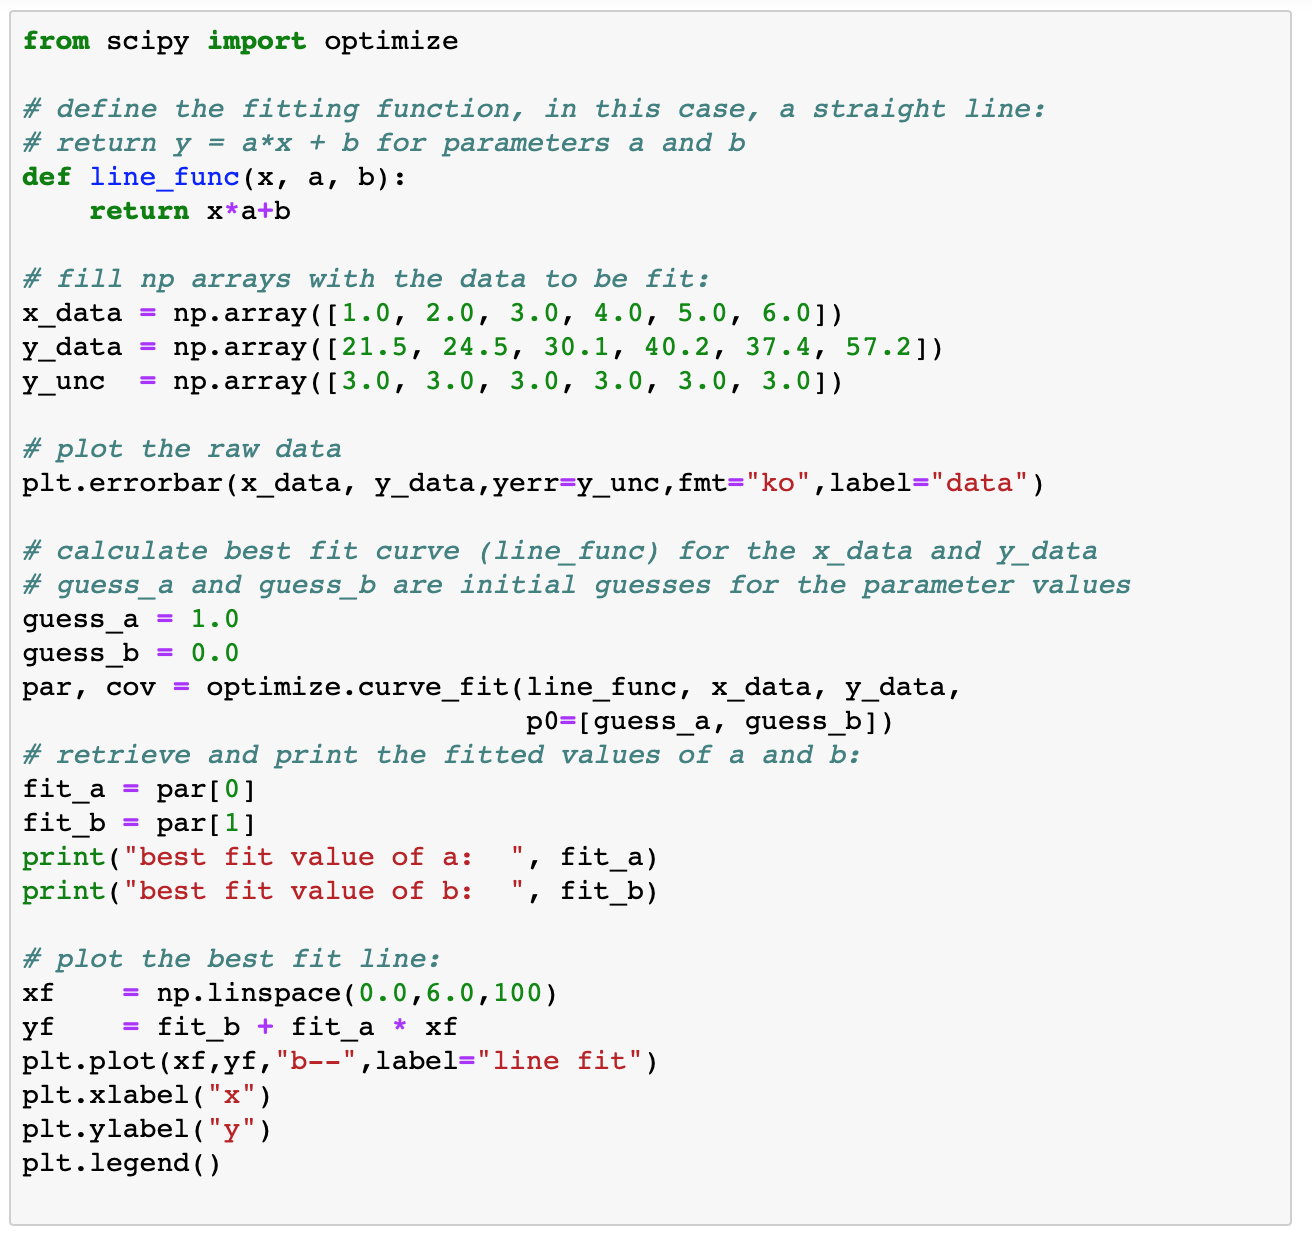
\includegraphics[width=0.65\textwidth]{figs/labs/fitting/fit_code.png} \\
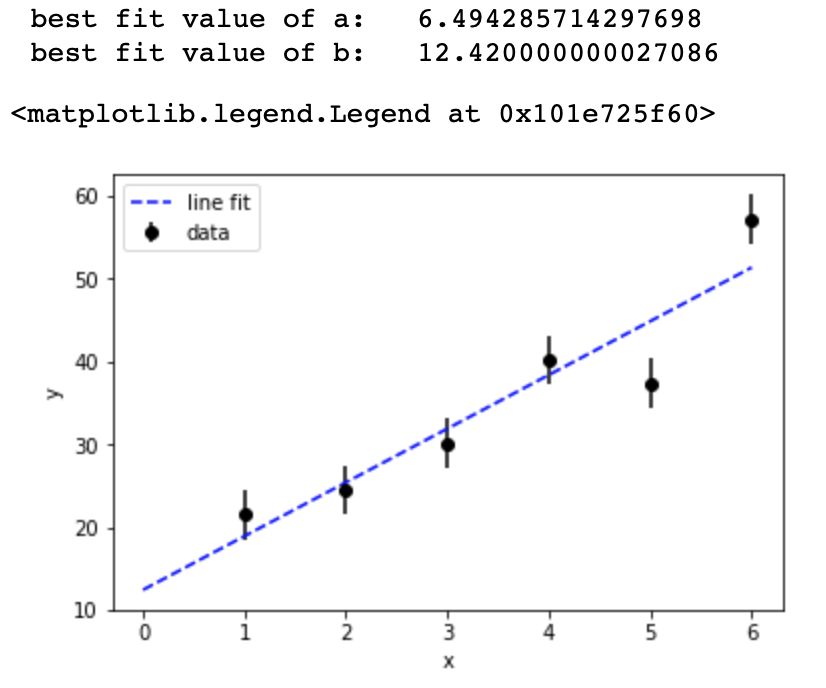
\includegraphics[width=0.65\textwidth]{figs/labs/fitting/fit_out.png} \\
\caption{Example fitting data to straight line.}
\label{fig:fiteg}
\end{center}
\end{figure}

An example using Scientific Pythons {\tt curve{\_}fit} function to fit
a straight line to data is shown in Fig.~\ref{fig:fiteg}.  A block of 
code defining the function we wish to fit, in this case, a straight
line, is defined as a function:
\begin{verbatim}
     def line_func(x, a, b):
         return a*x + b
\end{verbatim}
In this case, the function requires three parameters (in the computer
science sense) the x data in a numpy array as function parameter x,
the slope as function parameter a, and the intercept as function
parameter b.  When called, the function returns the x data multiplied
by the value a, with the value b added.  We don't directly call this
function, but in principle, it could be called like:
\begin{verbatim}
    y_data = line_func(x_data, 2.0, 0.0)
\end{verbatim}
to create a numpy array {\tt y{\_}data} constructed from {\tt
  x{\_}data} with slope 2 and intercept 0.

The next section filling numpy arrays containing the data, and
plotting it with error bars should be familiar by now.  The fit itself
is performed by the line:
\begin{verbatim}
par, cov = optimize.curve_fit(line_func, x_data, y_data, p0=[guess_a, guess_b])
\end{verbatim}
This performs a fit of the function {\tt line{\_}func} defined above
to the $x$ and $y$ data contained in the arrays {\tt x{\_}data} and
{\tt y{\_}data}.  Numerical fits generally find the local minimum,
which is not necessarily the global minimum of interest.  It is
important therefore, especially for complicated fits, to provide an
initial guess near the expected fit values.  These are provided to the
optional, named, function parameter {\tt p0}, which is set to the
python list {\tt [guess{\_}a, guess{\_}b]} which contains our initial guesses for
the fit parameters $a$ and $b$.  The function performs a least-squares
fit to find the best values of $a$ and $b$ which are returned as the
numpy array {\tt par}.  The function also returns the covariance
matrix as the numpy array {\tt cov}.

The remaining code simply uses the best fit values to plot the fitted
function as a dashed line.  Numerical fits are fickle.  Even if you
are only interested in the fitted value, you should always plot the
best-fit function and compare the results to your data as in important
check for your work.

\begin{table}
\caption{Sample data for straight line fit.}
\label{tbl:linesamp}
\begin{center}
\begin{tabular}{ll}
$x$ & $y \pm \sigma_y$ \\
1.0  & $15.9 \pm 3.0$ \\
2.0  & $23.6 \pm 3.0$ \\
3.0  & $33.9 \pm 3.0$ \\
4.0  & $39.7 \pm 3.0$ \\
5.0  & $45.0 \pm 10.0$ \\
6.0  & $32.4 \pm 20.0$ \\
\end{tabular}
\end{center}
\end{table}

%\begin{figure}[htbp]
%\begin{center}
%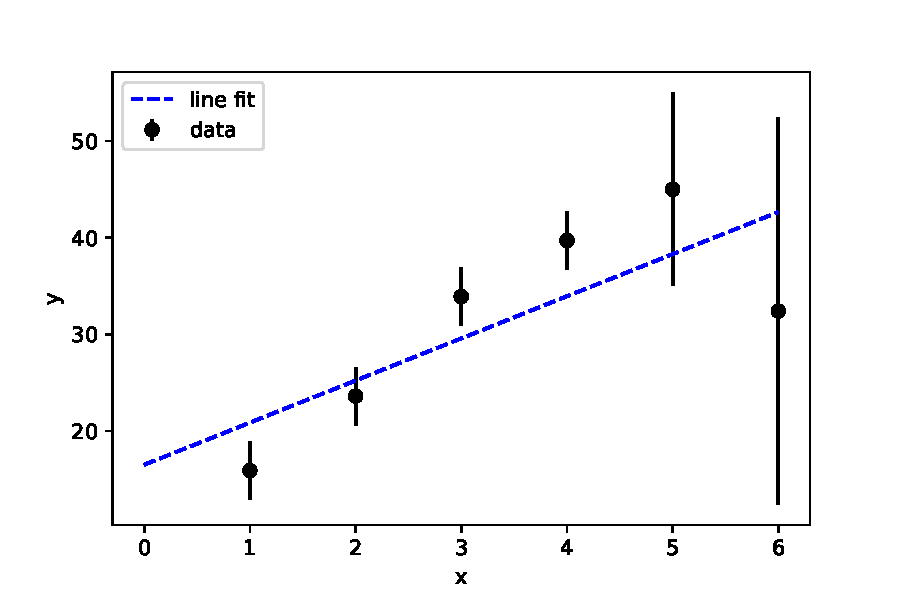
\includegraphics[width=0.65\textwidth]{figs/labs/fitting/bias.pdf} 
%\caption{This linear fit is biased by the failure to properly account for uncertainties.}
%\label{fig:fitbias}
%\end{center}
%\end{figure}

\begin{plot} Apply a code like that of Fig.~\ref{fig:fiteg}
to the data in Table~\ref{tbl:linesamp}. Plot the data including error bars and the best-fit function.
% reproduce the plot in Fig.~\ref{fig:fitbias}.  
\end{plot}

Notice that the last two data points have larger uncertainties than
the other data points.  However, the call to the {curve{\_}fit}
function does not provide the parameter uncertainties, and so the
function assumes that they all have the value $1$.  In this case,
since the uncertainties are not in fact all the same, the function
does not find the correct minimum.  The answer is clearly biased
toward the poorly measured points, because the function gives these
points the same weight as all of the other points.

\begin{print} The {\tt curve{\_}fit} function does not provide directly the $\chi^2$ value of the fit. However you can calculate it manually via equation~\ref{eqn:chi2}. The sum can be obtained via numpy function sum. Modify your code to include calculation of the $\chi^2$ value of the fit. Include also the calculation of the $\chi^2$ divided by the number of degrees of freedom (number of data points minus number of parameters), which is called reduced $\chi^2$. Print both of those values. Is the fit reasonable based on the reduced $\chi^2$ value? Print your comment as well. 
\end{print}

\begin{plot} Look-up the {\tt curve{\_}fit} function and the optional parameter
{\tt sigma}. Provide the correct uncertainties to
the fit and make a new plot with the data and the fit.  You should observe that the fit results is no longer biased,
and more closely tracks the well constrained left side of the plot. \end{plot}

\begin{print} Print $\chi^2$ and reduced $\chi^2$ value. Is the fit reasonable based on the reduced $\chi^2$ value? Print your comment as well. \end{print}

\section{Parameter Uncertainties I}
\label{sec:sigmatrue}
As discussed in the lecture the uncertainty $\sigma_{p_i}$ on the $i$th parameter $p_i$
can be determined from the second derivative of the $\chi^2$ function:
\begin{displaymath}
\frac{d^2\chi^2}{d p_i^2} = \frac{2}{\sigma_{p_i}^2}.
\end{displaymath}
In general, for $M$ parameters, the $M \times M$ covariance matrix is calculated as:
\begin{displaymath}
C(i,j) = 2 \cdot \left(\dfrac{d^2\chi^2}{d p_i d p_j} \right)^{-1}
\end{displaymath}
from which we can see that the diagonals are simply the parameter uncertainties squared:
\begin{displaymath}
C(i,i) = 2 \cdot \left(\dfrac{d^2\chi^2}{d p_i^2} \right)^{-1} = \sigma^2_{p_i}.
\end{displaymath}
The off-diagonal elements contain information about how parameters are
correlated, and for a well designed fit function they should be close to
zero.

The {\tt curve{\_}fit} function returns both the best fit parameter values and the covariance matrix:
\begin{verbatim}
par, cov = optimize.curve_fit(...)
\end{verbatim}
For a fit with $M$ parameters, we can obtain an array containing the
$M$ parameter uncertainties from the square root of the diagonals of the $M \times M$
covariance matrix:
\begin{verbatim}
unc = np.sqrt(np.diag(cov))
\end{verbatim}

We can obtain uncertainties of parameters by accessing elements of the array.

Lets study this in an example for $N=1$ parameter. Generate $x$-values as a numpy array of evenly spaced values from 0 to 99. Generate $y$-values as 100 random numbers drawn from a Gaussian distribution with mean $m = 50$ and a width $\sigma_y =10$.  Perform a fit using {\tt curve{\_}fit} function. Set the uncertainties on the $y$ values to 10 and also set parameter {\tt absolute{\_}sigma = True}.  

 The best fit constant value we expect is simply the mean of the $y$-values.  The
uncertainty on the mean value should be:
\begin{displaymath}
\sigma_m = \sigma_y / \sqrt{N} = 10 / \sqrt{100} = 1.0
\end{displaymath}

\begin{print} Calculate the expected values for the best fit value and its uncertainty. Print them together with the fitted best fit value and its uncertainty. Do those agree? \end{print}


\section{Fitting a Sine Curve}

In this section, you will fit the sample data to a sine function:
\begin{displaymath}
 y = A \, \sin( k x). 
\end{displaymath}
Use the following sample data:\\
\begin{center}
\begin{tabular}{|ll| ll|ll|}
\hline
$x$ & $y$ & $x$ & $y$ & $x$ & $y$\\
\hline
0  & 5.3    & 4  & -9.7   & 8  & 15.7  \\
1  & 15.0   & 5  & -17.4  & 9  & 18.5  \\
2  & 19.2   & 6  & -20.5  & 10 & 8.6   \\
3  & 6.8    & 7  &  2.1   & &  \\
\hline
\end{tabular}
\end{center}
Assume the uncertainty is the same for each $y$ value: $\sigma_i = 2$.
\begin{plot} Plot the data including error bars and the best-fit
sine wave. \end{plot}

\begin{print} Print the best fit parameter
values and their uncertainties. \end{print}

Remember to set {\tt absolute{\_}sigma=True}.\\

This is a \textbf{sign-off point} for this lab. 

\section{Parameter Uncertainties II}

%\begin{figure}[htbp]
%\begin{center}
%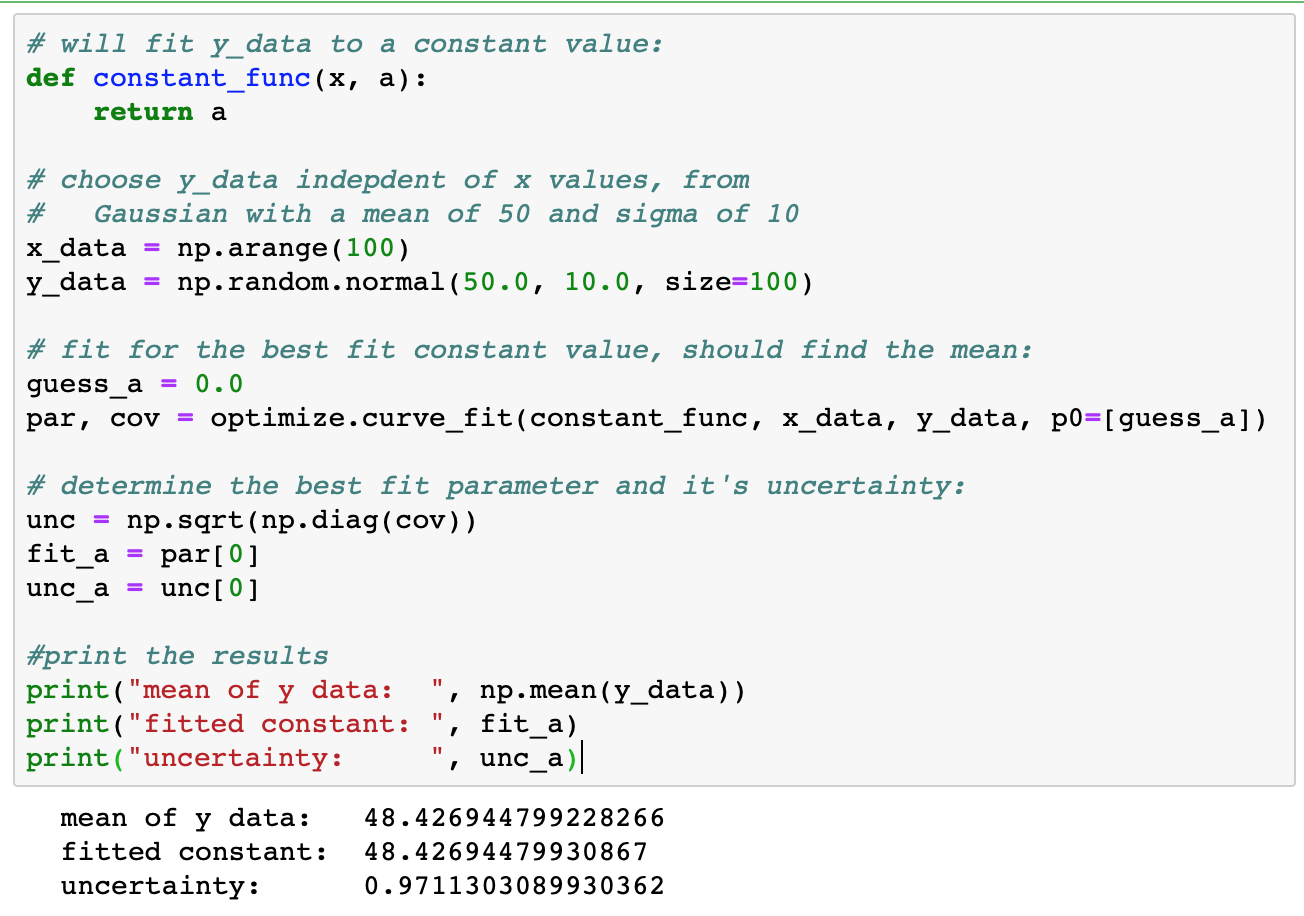
\includegraphics[width=0.65\textwidth]{figs/labs/fitting/uncertainties.png} \\
%\caption{Example obtaining parameter uncertainties.}
%\label{fig:fitunc}
%\end{center}
%\end{figure}

Lets repeat the study in~\ref{sec:sigmatrue}. Generate $x$-values as a numpy array of evenly spaced values from 0 to 99. Generate $y$-values as 100 random numbers drawn from a Gaussian distribution with mean $m = 50$ and a width $\sigma_y =10$.  Perform a fit using {\tt curve{\_}fit} function.  Leave the uncertainties on the $y$ values
unspecified and also leave parameter {\tt absolute{\_}sigma} unspecified. 

\begin{print} Print the fitted best fit value and its uncertainty. \end{print}

It's surprising actually, that the fit returns the correct
uncertainty.  Your code does not provide  the uncertainty on the $y$ parameters $\sigma_y$ to
the fit.  So how can it possible deduce the correct uncertainty
$\sigma_m = \sigma_y / \sqrt{N}$?

The answer is that behind the scenes, the {\tt curve{\_}fit} function
is being really quite clever (too clever, in my opinion, for a default
behavior!)  By default, the covariance matrix returned by the 
{\tt curve{\_}fit} function is scaled by the factor:
\begin{displaymath}
\alpha = \frac{\chi^2_{\rm min}}{\rm NDF}
\end{displaymath}
the minimum value of the $\chi^2$ divided by the number of degrees of
freedom (number of data points minus number of parameters).  As discussed in lecture that $\alpha$ is around 1 for a least-squares fit with
an appropriate model and correct uncertainties.  So nominally this
factor is one, and has no effect.  But consider what happens if the
actual uncertainties are $\sigma$ while the $\chi^2$ used in the fit assumes they
are, for example, ``1''.  In this case, the calculated $\chi^2$ is:
\begin{displaymath}
\chi^2 = \sum_i \frac{(f(x_i;p) - y_i) ^2}{1}
\end{displaymath}
which differs from the correct $\chi^2$:
\begin{displaymath}
\chi^2 = \sum_i \frac{(f(x_i;p) - y_i) ^2}{\sigma^2}
\end{displaymath}
by a factor of $\sigma^2$.  This means that while the correct value
for $\alpha$ is nearly one, the calculated value of alpha will be
$\sigma^2$.  This is precisely the factor needed to scale the squared
parameter uncertainties to account for the fact that the initial
uncertainty was $\sigma$ but we assumed $1$.

This behavior is controlled by the parameter {\tt absolute{\_}sigma}.
By default, the function sets {\tt absolute{\_}sigma = False} and
scales the covariance matrix as just described.  On the other hand, if
you want to simply use the provided uncertainties without re-scaling
the covariance matrix, you must remember to set {\tt
  absolute{\_}sigma = True}.  I think this is a really poor choice of
default behavior...  it's really quite a fancy thing to do implicitly.
In cases when you know the uncertainty on your data points, this
re-scaling actually results in less correct estimate for the
uncertainties.  This is because for a good model with proper
uncertainties, the factor $\alpha$ is near one, but not exactly one.

\begin{print} Repeat the study but leave the uncertainties on the $y$ values
unspecified and set {\tt absolute{\_}sigma = True} in the fit.  You
should obtain an uncertainty of $0.1$.  Print your value and print your explanation of
why you obtained this value. \end{print}

As a rule of thumb, when using {\tt curve{\_}fit}, if you provide
explicit uncertainties, you should remember to set {\tt
  absolute{\_}sigma = True}.  And really, for precision work, you should
almost always be providing explicit uncertainties.



















\documentclass[12pt,oneside]{book}

\usepackage[dvips,letterpaper,margin=0.75in,bottom=0.75in]{geometry}
\usepackage{cite}
\usepackage{slashed}
\usepackage{graphicx}
\usepackage{amsmath}
\usepackage{enumitem}

\usepackage[american,fulldiode]{circuitikz}
\tikzset{component/.style={draw,thick,circle,fill=white,minimum size =0.75cm,inner sep=0pt}}

\begin{document}
\ctikzset{bipoles/thickness=1}
\ctikzset{bipoles/length=.6cm}

\title{Physics 80 Lab Manual}

\maketitle

\chapter{The Speed of Light in Air }

\section{Pre-lab Calculations}
\noindent
1) Suppose .  Hint: assume a . \\ 

\noindent
2)   \\

\noindent
3) What is the definition of the meter ? What is the exact value of the speed of light in vacuum?
%The meter  is the length of the path travelled by light in vacuum during a time interval of 1/299792458 second. The exact value for the speed of light in vacuum is 299,792,458 metres per second.

\section{Introduction}

In this lab, you will measure the speed of light in the air by measuring the time between sending and receiving a flash of light over a known distance, evaluate statistical and systematic uncertainties and compare it to the known value.  In the process, you will learn how to use your scope to make time measurement.

The flash of red light is created by a pulsed laser diode, a device very similar to a laser pointer, except this laser is switched on and off (pulsed) at a very high rate: 1 million times per second (1 MHz).  Whenever laser diode is pulsed a "trigger" pulse is sent to the oscilloscope. The pulsed beam of light is detected by a fast photo-diode detector and a "signal" pulse is sent to the oscilloscope. The time difference between the two pulses $\Delta t$ can be measured as a function of the distance $L$ between the laser/detector apparatus. 
Assuming that the time difference between the two pulses depends only on the time it took the light to travel the distance $L$ one can determine the  phase velocity of laser diode light in the air:   $v_{red}=\frac{L}{\Delta t}$.


%and the
%mirror
%can be bounced off of
%a mirror and the return pulses detected by a very responsive (“fast”) detector. Each pulse of the laser
%creates two signals, one from the laser itself (the “trigger”) and one from the detector when it picks up the
%returning pulse. These two signals can be compared to each other with a fast oscilloscope, and the time
%between them can be measured as a function of the distance between the laser/detector apparatus and the
%mirror. By varying the total distance from the laser to the detector L and monitoring the time difference
% on the scope, one can determine the speed of light c. If the time difference between the two signals 
%depended only on the time it took for the light to travel that distance, then c would be given by


\section{Measuring the $I$-$V$ Curve of a Diode}

In this section you will measure the $I$-$V$ curve of a 1N914 diode, and compare your results to the curves available from the device data sheet.  To avoid taking a bunch of measurements by hand, we will use a trick to plot the curve directly on your oscilloscope using the XY mode.
\begin{figure}[htbp]
\begin{center}
\begin{tabular}{c@{\hskip 2cm}c}

\begin{circuitikz}[line width=1pt]
\draw
(0,0) to[sinusoidal voltage source,bipoles/length=1.5cm,l=$\tilde{V}$] (0,4) -- (2,4);
\draw
(2,4) node[right]{$P_2$} to[resistor,l=$R_1$,o-o] (2,2) node[right] {$P_1$} to[diode,l=$D_1$,-o](2,0) node[right]{G}-- (0,0)
;
\draw (0,0) -- ++(0,0) node[ground,yscale=2.0]{};
\end{circuitikz} &

\begin{circuitikz}[line width=1pt]
\draw
(0,0) to[sinusoidal voltage source,bipoles/length=1.5cm,l=$\tilde{V}$] (0,4) -- (4,4);
\draw
(2,4) to[resistor,l_=$R_1$,*-o] (2,2) node[left]{$P_1$} node[right]{(Ch.1)} to[diode,l_=$D_1$,o-*] (2,0)
(4,4) to[diode,l=$D_2$,-o] (4,2) node[right] {$P_2$ (Ch.2)} to[resistor,l=$R_2$,-o](4,0) node[right]{G}-- (0,0)
;
\draw (2,0) -- ++(0,0) node[ground,yscale=2.0]{};
\end{circuitikz} \\
(a) & (b) \\
\end{tabular}
\caption{Diode circuits for (a) demonstrating rectification and (b) plotting the diode IV curve on your oscilloscope.}
\label{fig:diodecircuits}
\end{center}
\end{figure}

Consider (but don't build!) the circuit in Fig.~\ref{fig:diodecircuits}a.  The voltage between points $P_2$ and $P_1$ is proportional to the current passing through the diode, and the voltage between points $P_1$ and $G$ is the voltage across the diode.  So if we could display $P_2-P_1$ versus $P_1-G$ on your scope we could use this circuit.  Unfortunately, this is not possible on your scope, because (1) the only valid place to put the scope probe ground shield clips is at the point $G$ (Why?) and (2) you can only display Channel 1 versus Channel 2 in XY mode.   

The solution is to drive two copies of the diode in series resistor, with the component order reversed, as in Fig.~\ref{fig:diodecircuits}b.  This way, we can connect the probe ground shields as required at point $G$, put the voltage across the diode on scope Channel 1 by connecting the probe tip at $P_1$, and put the voltage across the resistor (proportional to current through the diode) on scope Channel 2 by connecting the probe tip at $P_2$.

Build the circuit in Fig.~\ref{fig:diodecircuits}b using a 1N914 fast switching diode for $D_1$ and $D_2$ and $R_1= R_2 = 10~{\rm k\Omega}$.  Set your function generator for high-impedance output, providing AC with peak to peak voltage of $20~\rm V$ at a frequency of $100~\rm Hz$.  Before switching to XY mode, make certain that your Channel 1 has no voltage offset (that is, zero voltage is located at the origin) or else your diode output voltage won't be calibrated properly in your output plot.   Once you set this, try not to adjust the offset of Channel 1 or you'll have to redo it!  To minimize noise, set the bandwidth limit ``On'' for both channels (this is available in the menu for each input channel as ``BW Limit'').

\begin{figure}[htbp]
\begin{center}
\begin{tabular}{c@{\hskip 2cm}c}
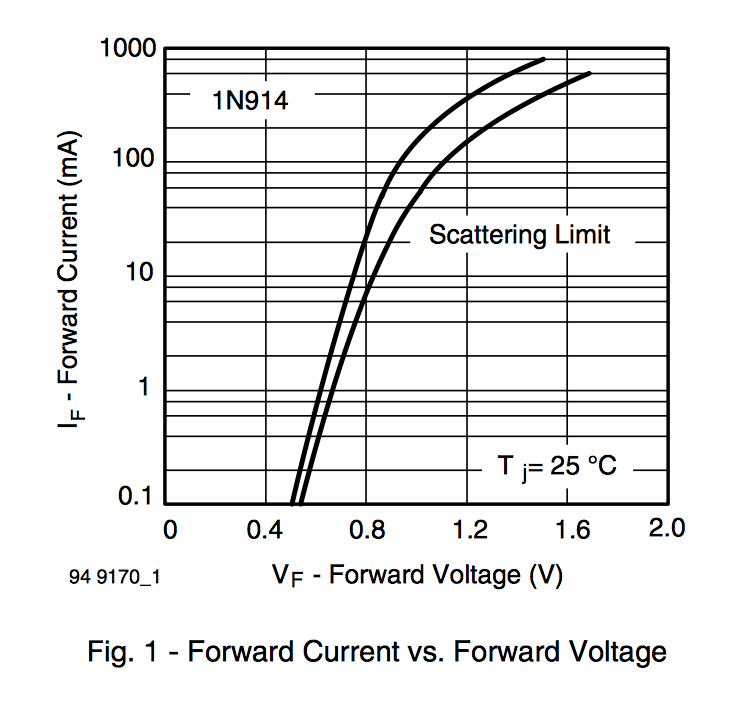
\includegraphics[height=0.25\textheight]{figs/labs/diode/1N914.png} &
\begin{picture}(200,100)
\put(0,0){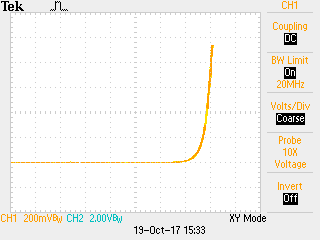
\includegraphics[height=0.25\textheight]{figs/labs/diode/diodeiv.png}}
\put(10,52){$0~mA$}
\put(10,70){$0.2~mA$}
\put(10,88){$0.4~mA$}
\put(10,106){$0.6~mA$}
\put(10,124){$0.8~mA$}
\put(10,142){$1.0~mA$}
\end{picture}\\
(a) & (b) \\
\end{tabular}
\caption{\label{fig:diodeiv} IV curves for the1N914 from (a) data sheet, and (b) as you will measure in this lab.  In the scope trace, the Channel 2 ($Y$) with scale set to $2~\rm V$ measures the voltage across a $10~\rm k\Omega$ resistor, so each division corresponds to $200~\rm \mu A$ as indicated. 
}
\end{center}
\end{figure}

Set the scope into XY mode, and see if you can reproduce the diode IV curve in Fig~\ref{fig:diodeiv}b.
Beats jotting down voltages in your logbook doesn't it?  Now jot down the voltage you expect across the diode for a current of $1~\rm mA$ in your logbook.  Where they overlap, does your measured IV curve agree with the curve from the component data sheet in Fig.~\ref{fig:diodeiv}a?

\section{Rectifying an AC Signal}

\begin{figure}[htbp]
\begin{center}
\begin{circuitikz}[line width=1pt]
\draw
(0,0) to[sinusoidal voltage source,bipoles/length=1.5cm,l=$\tilde{V}$] (0,4) -- (2,4)
(2,4) node[right]{$P_2$} to[diode,l=$D$,o-o] (2,2) node[right] {$P_1$} to[resistor,l=$R$,-o](2,0) node[right]{$G$} -- (0,0)
(2,0) -- ++(0,0) node[ground,yscale=2.0]{};
\end{circuitikz} 
\caption{A diode rectification circuit.}
\label{fig:rect}
\end{center}
\end{figure}

Set your function generator to provide an AC source with frequency $100~\rm Hz$ and peak-to-peak voltage $V_{\rm pp}=5~\rm V$.  Build the circuit in Fig.~\ref{fig:rect} using a 1N914 diode for $D$ and $R=1.8~\rm k\Omega$. 

With your scope probe ground shield clips both properly connected to the ground at $G$, monitor the voltage at points $P_1$ and $P_2$.   Sketch the voltage across the resistor $R$ and the voltage supplied by the function generator versus time on the same plot in your lab book. 

Using your scopes amplitude measurement feature, measure precisely (i.e. to within $50~\rm mV$ precision) the voltage drop across the diode at the peak current value, by measuring the difference between Channel 1 and Channel 2 of your scope at the peak.  Is this operating point consistent with your results from the previous section and the pre-lab calculations?


\section{Lab Report}

Your report should include all of your measurements and a comparison with your calculation.
 

\end{document}


%\chapter{Statistics of Radioactive Decays}


\section{Introduction}

\begin{figure}[htbp]
\begin{center}
 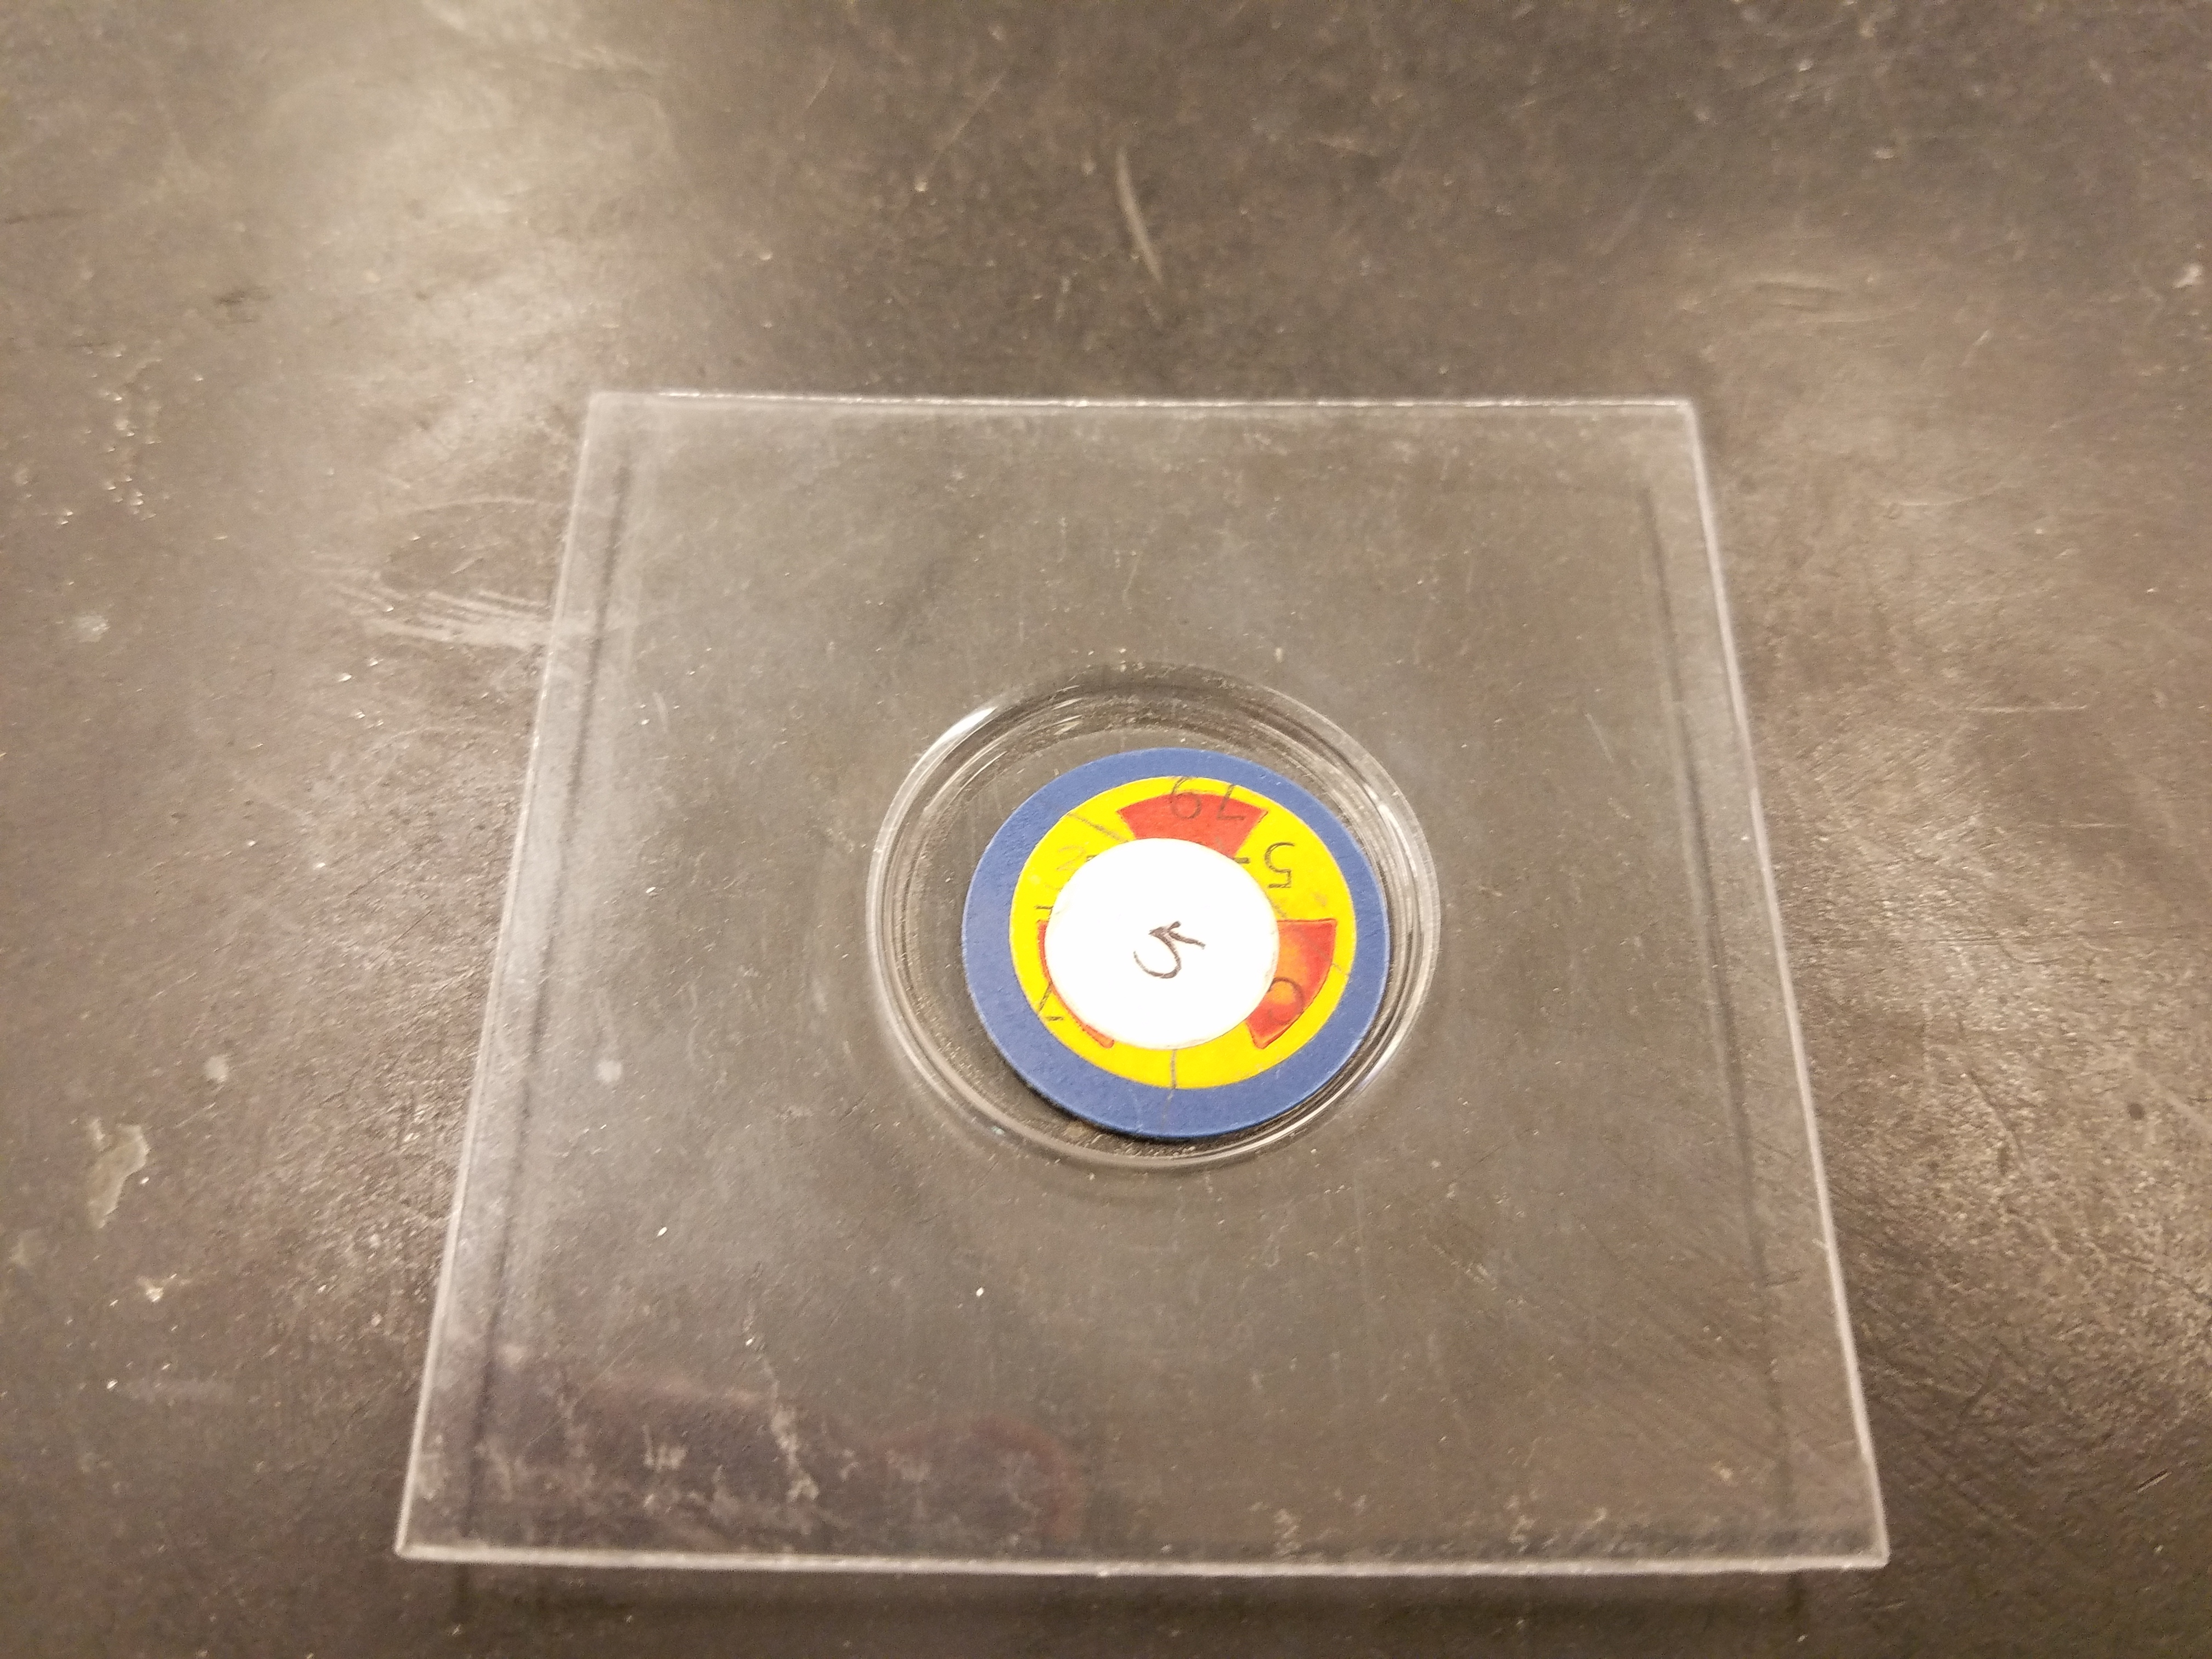
\includegraphics[width=0.55\textwidth]{figs/labs/geiger/source.jpg};
\caption{\label{fig:source} A sealed radioactive source.  A small
  amount of Cs-137 is contained within the small button shaped piece
  of plastic.  For your safety, the sources will be handled only by
  the TA.}
\end{center}
\end{figure}

In this lab, you will use a Geiger Counter to study the statistics of
radioactive decays.  For this lab there are both logbook and Jupyter
notebook entries.

\section{Precautions}

\noindent
{\bf Precautions with the Geiger counter:}
\begin{itemize}
\item Leave the cable from the Geiger counter controller to the Geiger
  counter in place {\em at all times}.  This carries voltages of
  approximately 1000 volts.  If you leave the cable in place, nothing
  can be inadvertently plugged in (including fingers).
\item Leave the Geiger tube in its holder.  It has a thin front window
  which is easily broken.
\item Do not set the high voltage higher than 1000 volts.
\end{itemize}

\noindent
{\bf Precautions with the radioactive source:}
\begin{itemize}
\item See Fig.~\ref{fig:source} to familiarize yourself with what the sources look like.
\item Don't touch the source.
\item Leave the source in the tray at all times.  The TA will provide
  the sources and handle moving them from place to place.
\item Radiation falls off as $1/r^2$.  So minimize your time near
  sources and maximize your distance from them.
\end{itemize}

\section{The Geiger Counter}

\begin{figure}[htbp]
\begin{center}
\begin{tikzpicture}
    \node[anchor=south west,inner sep=0] (image) at (0,0,0) {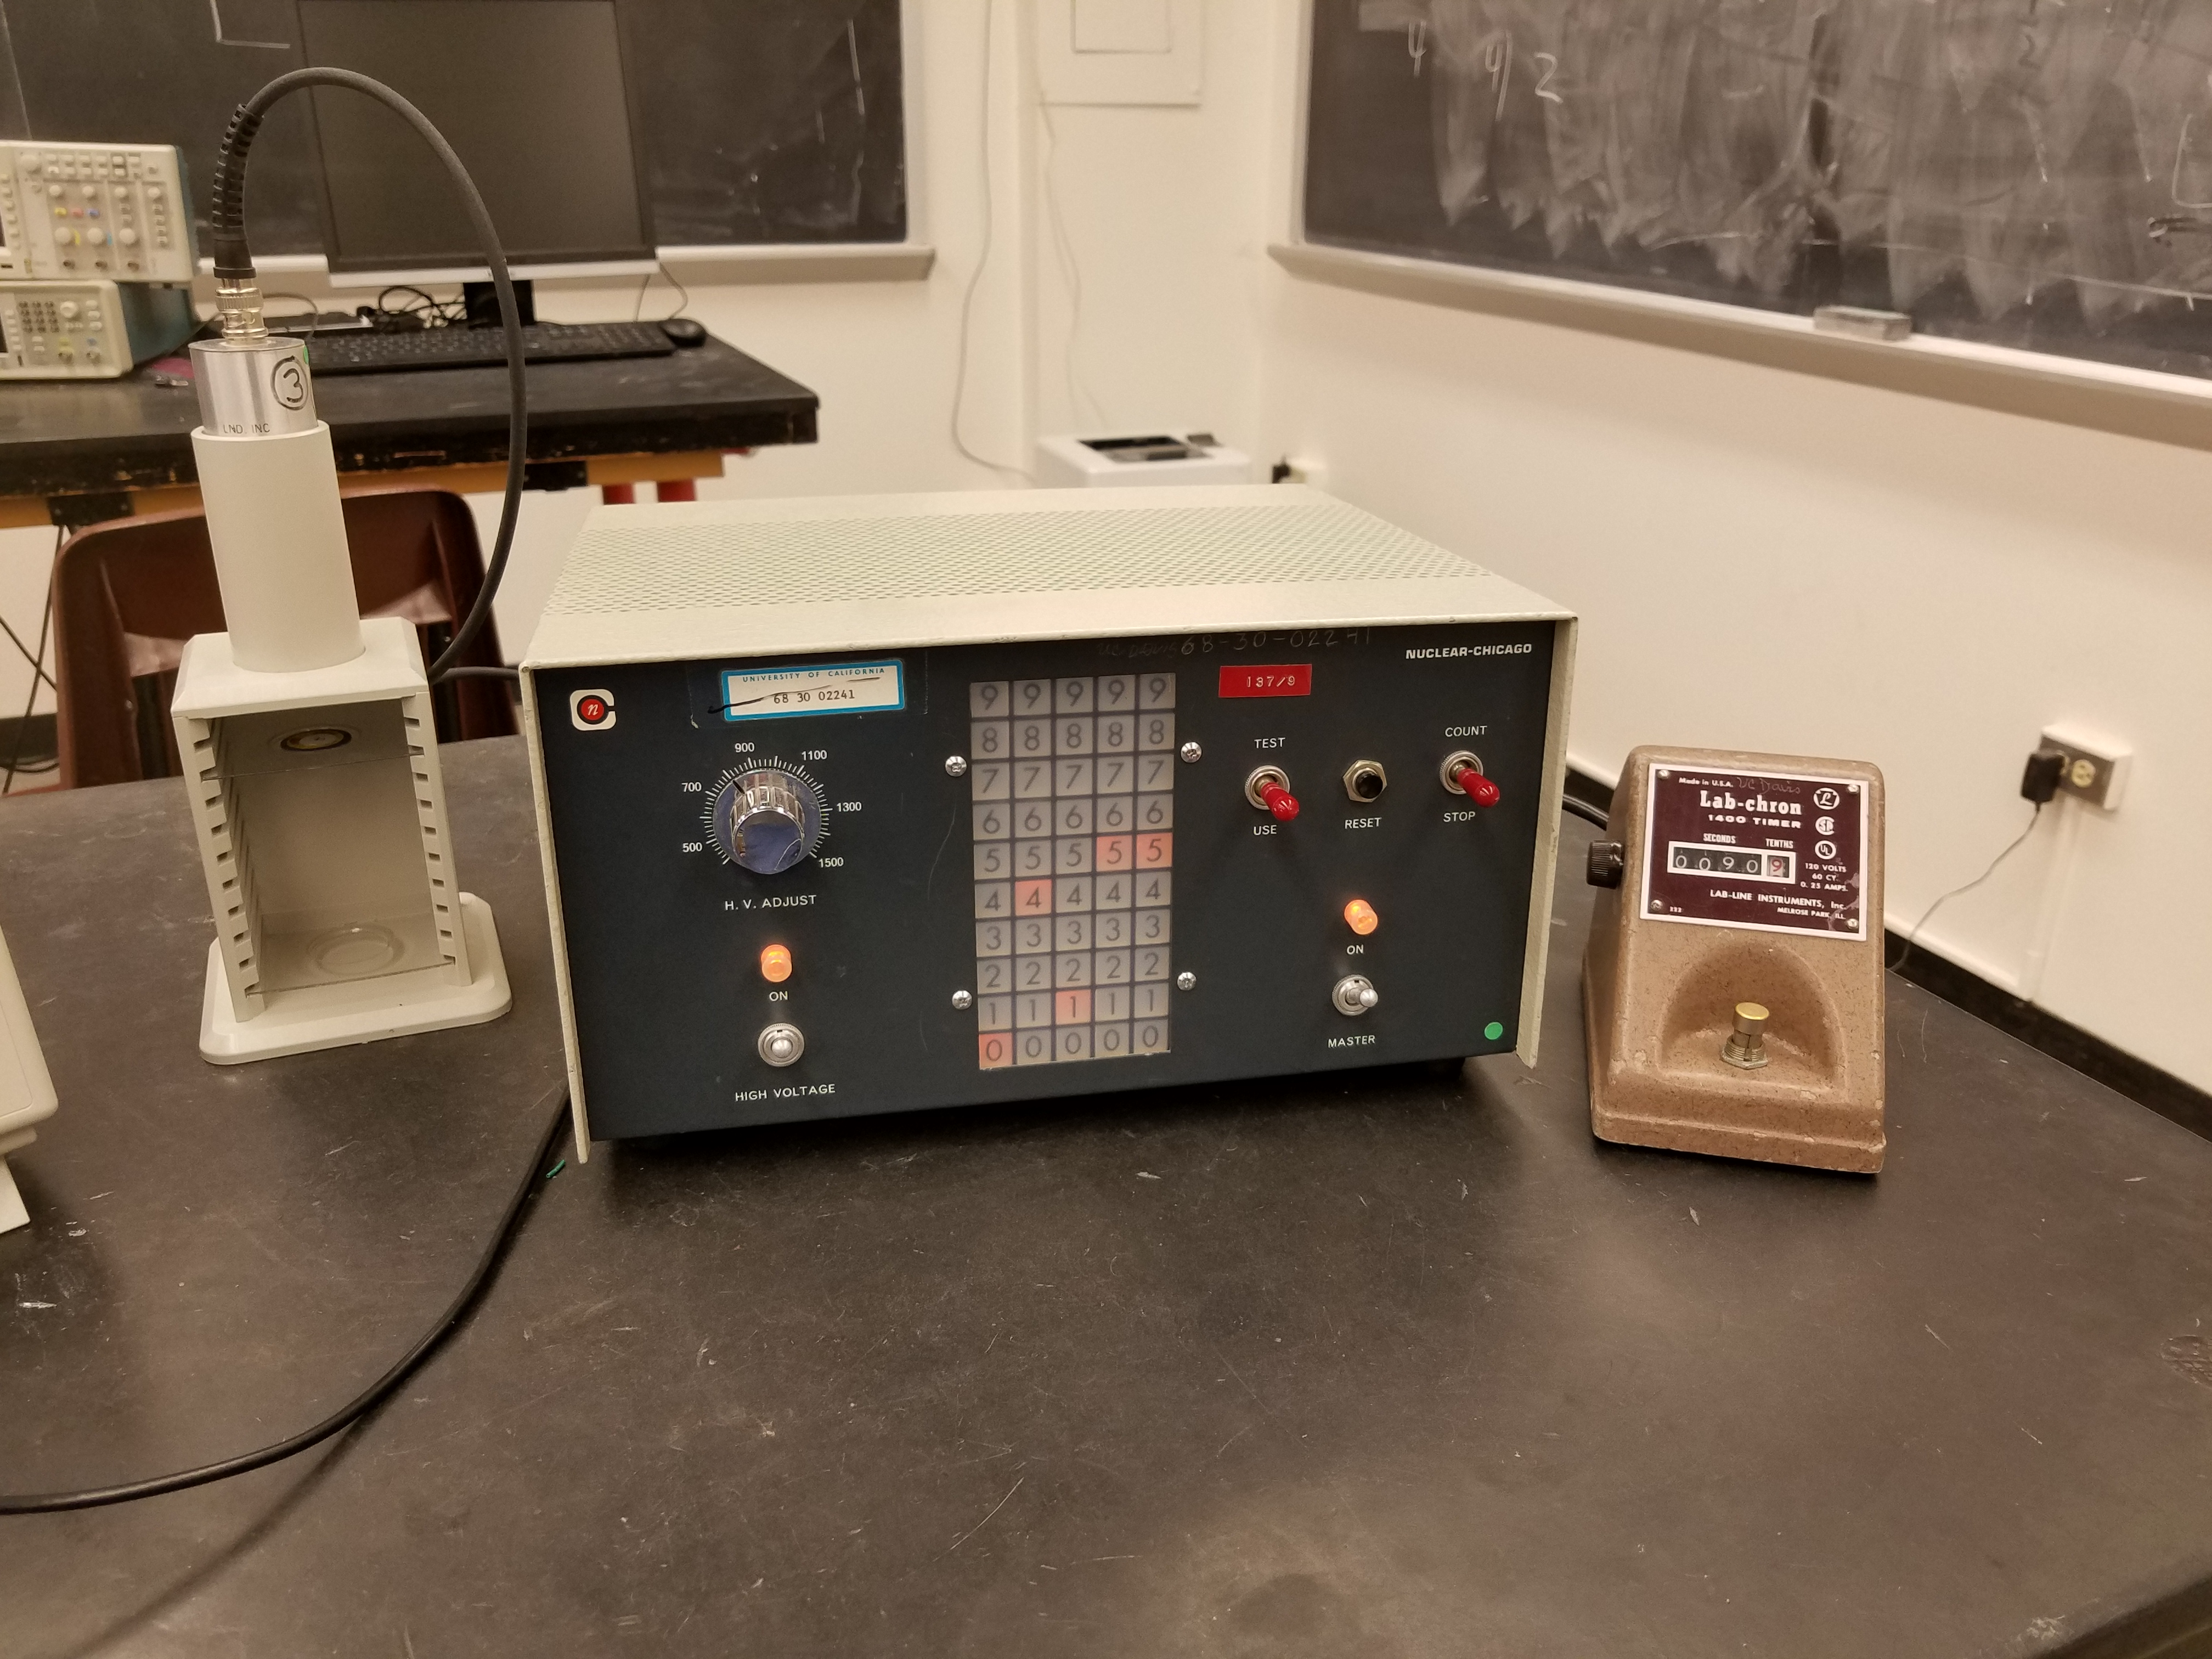
\includegraphics[width=0.55\textwidth]{figs/labs/geiger/assembly.jpg}};

    \node[right](X) at (10.0,3.0) {Timer};
    \draw (X.west) -- (8.0,3.5);

    \node[right](X) at (10.0,5.0) {\parbox{3cm}{\flushleft High-Voltage and Counter}};
    \draw (X.west) -- (5.0,4.75);

    \node[left](X) at (0.0,4.5) {\parbox{2.5cm}{\flushright Geiger Tube Holder}};
    \draw[white,thick] (X.east) -- (1.25,5.0);
    \draw (X.east) -- (1.25,5.0);

    \node[left](X) at (0.0,3.0) {Source};
    \draw (X.east) -- (1.35,4.05);

\end{tikzpicture}
\caption{\label{fig:geigersetup} The Geiger Counter assembly.}
\end{center}
\end{figure}

To begin, familiarize yourself with the counter and timer features of
your Geiger counter assembly using the built-in test mode.  Your lab
bench will already be prepared with a Geiger Counter assembly as shown
in Fig.~\ref{fig:geigersetup}.  Ensure that the high-voltage (HV) is
off by turning the knob labeled ``H.V. Adjust'' counter-clockwise all
the way to zero.  Now put the Geiger counter into test mode by
flipping the left red switch to ``TEST''.  Flip the right red switch
to ``COUNT'' and you should see the counter display begin
incrementing.  Push the button on the front of your timer and you
should see the Timer turn on and off.  Leave the timer incrementing.
Now flip right red switch to ``STOP'', and observe that the both the
counter and the timer stop simultaneously.  The knob on left side of
the old-school lab timer can be used to reset the time.  Keep turning
the knob clockwise until the time reads 0.  Use the black button on
the Counter to reset the count to zero.

Flip the right switch to ``COUNT'' and then back to ``STOP'' when 10
seconds have passed.  During this time, the $60~\rm Hz$ test signal
should increment the counter close to 600 times.  Try this a few times
and make sure you can reliably count close to $600$ test pulses in a
10 second interval.  You should reset the count each time, but there
is no need to reset the timer.  Simply stop when the timer reaches the
next factor of ten.  Due to your reaction time, you may well stop at
one-to-two tenths of a second later.  This is OK, and will only add
less than a few percent error to your measurements over 10 second
intervals.

\section{High-Voltage Calibration}

When you are confident that you know how to operate the timer, switch
the left red switch to ``USE'' mode.  Unless a sealed radioactive
source is already in place, ask the TA to provide you with a source in
the second shelf from the top of your Geiger tube holder.  Switch the
right switch to ``COUNT'' mode.  With the HV off, you should not see
any pulses.  Turn the HV up until you begin to see counts increment on
the display, and continue to the next interval of 50 volts (e.g. if it
first starts incrementing at 730 volts, set the dial to 750 volts).
Count the number of events in a ten second interval.

Repeat this measurement in 50 volt steps up to 1000 volts.  Do not exceed 1000 volts.

\begin{plot}
Plot the rate (in Hz) as a function of high voltage.  You should see a
plateau region (a leveling off) which indicates the onset of the
Geiger mode within the Geiger tube.  The Geiger tube has some
resistance even in Geiger mode, so do not expect a perfectly flat
plateau.  From your plot, chose a high-voltage near the beginning of
the Geiger mode, and set the high-voltage to this calibrated value.
If you are struggling with Python, you can make a rough plot by hand
in your logbook to determine the plateau region, and leave the fancy
plot for later.
\end{plot}

\begin{figure}[htbp]
\begin{center}
 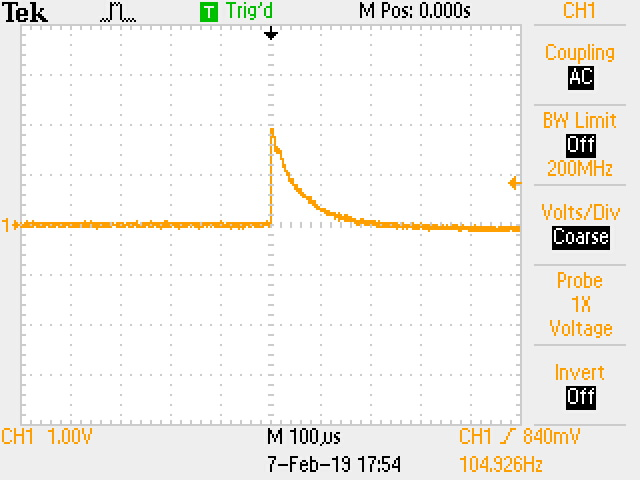
\includegraphics[width=0.55\textwidth]{figs/labs/geiger/pulse.jpg};
\caption{\label{fig:geigerpulse} An example Geiger counter pulse.}
\end{center}
\end{figure}

Connect an oscilloscope to the output of the counter assembly (on the
back, labeled ``SCOPE'').  Adjust your scope to view the Geiger pulses
like that of Fig.~\ref{fig:geigerpulse}.  Note that the Geiger counter
output contains a DC component in addition to the AC pulse, so you
will want to use your scope in AC coupling mode which will remove the
DC component and allow you to see the pulse.  You will also want to
see the attenuation to 1X because you are not using an attenuating
probe.

\begin{measurement}
Sketch a typical Geiger counter pulse in your logbook and indicates the pulse height and time duration.
\end{measurement}

\section{Data Collection}

Even in today's world of digital automation, it is still useful to
know how to collect a small amount (up to a few hundred data points)
of data manually.  Often in the lab, you have one-off measurements
that you would like to make without investing in automation.

In this section, you will collect data manually for about one hour.
Practice a routine with your lab partner that allows you to take and
record the data as fast as possible.  For instance, person A should
operate the counter, and person B should use the PC.  Person A turns
the counter on for ten seconds, turns it off, and says (quietly)
``OK''.  Person B records the value on the PC and says ``Go''.  Person
A resets the counter and continues.  Remember that there is no need to
reset the Timer each time, which would take too long, and which would
actually be counterproductive (if you consider the effect of a roughly
constant reaction time.) 

Practice your routine a few times, and make sure your count is near
1000 events in a ten second interval.  Then record 120 data points.

When you have finished recording your data with the radioactive
source, ask your TA to remove the source and return it to the
radioactive locker.

Now record an additional 120 data points with no source, to measure
the background radiation rate.  You should record around 3 background
counts per 10 second interval.

\section{Analysis}

\begin{figure}[htbp]
\begin{center}
\begin{tabular}{cc}
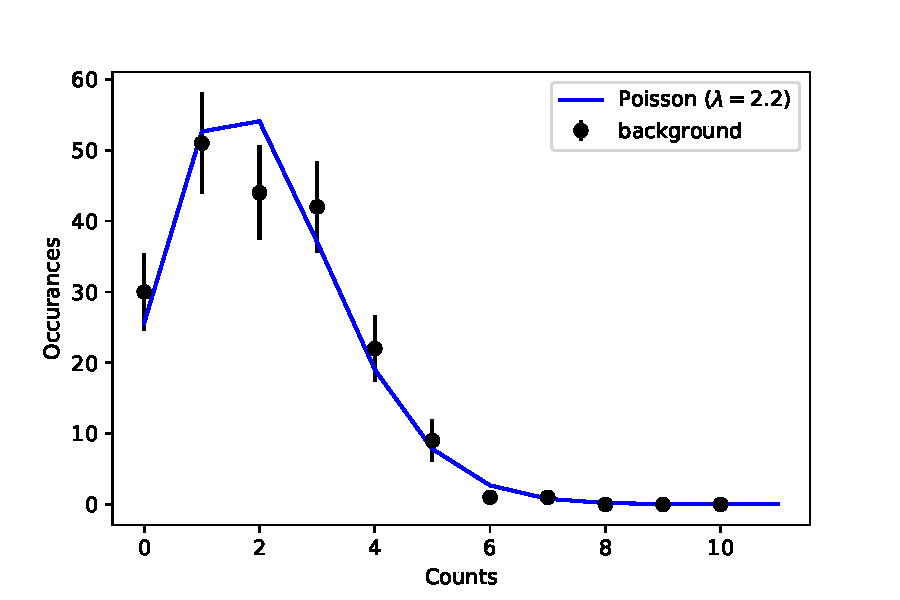
\includegraphics[height=0.22\textheight]{figs/labs/geiger/background.pdf}
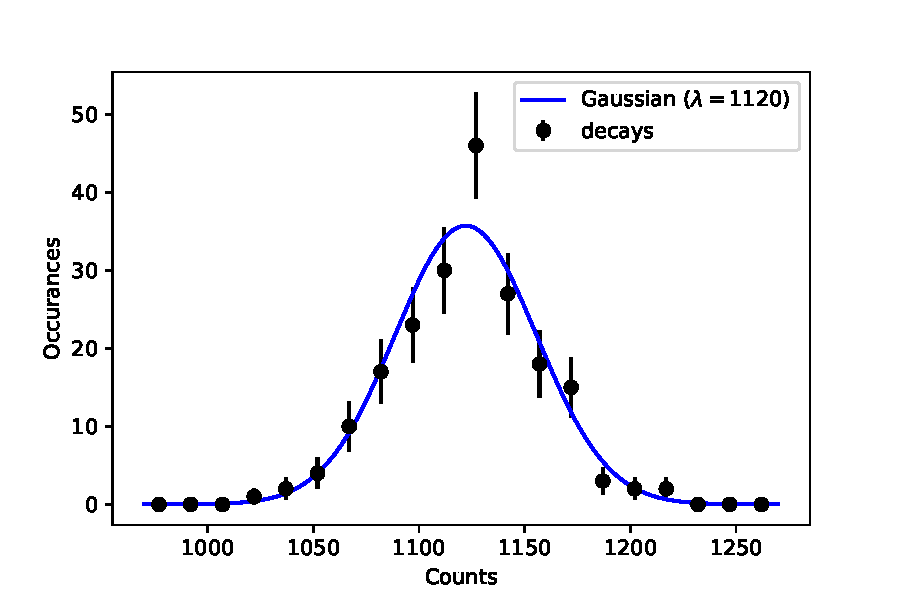
\includegraphics[height=0.22\textheight]{figs/labs/geiger/source.pdf}
\end{tabular}
\end{center}
\caption{\label{fig:geigeranalysis} Numerical simulation of the experiment
  for (a) background radiation only, and (b) radioactive source
  present.}
\end{figure}

Using Scientific Python, measure the mean and variance of your
collected background and source data.  Then produce histograms to
display your data as in Fig.~\ref{fig:geigeranalysis}.  For the
background data, plot the histogram for eleven bins: 0,1,2,...,10.
For the source data, plot about 20 bins covering a few hundred counts
around the mean value.

\begin{plot} Compare your collected background data to a Poisson distribution,
appropriately normalized, with a mean set to the mean of your data. \end{plot}
\begin{plot} Compare your collected source data to a Gaussian distribution,
appropriately normalized, with a mean set to the mean value of your
data, and sigma set to the square root of your mean. \end{plot}

This is a \textbf{sign-off point} for this lab. 
%move this earlier have them take data with source and analyze then sign off point plus data taking for only background plus analysis; so if they are late they get some plots that could be discussed.









%
\chapter{Measurement of Planck's Constant}

\section{Introduction}

In this lab, we will measure Planck's constant by measuring the
$V$-$I$ curves of three different colored light emitting diodes
(LEDs).  An LED is a particular type of diode for which the
recombination of electrons and holes produces photons, typically in
the visible light spectrum.  These diodes have an activation voltage given by:
\begin{equation} \label{eqn:va}
V_{\rm A} = \phi + \frac{hc}{e}\frac{1}{\lambda}
\end{equation}
where $\lambda$ is the wave-length of the light produced by the diode,
and $\phi$ is the contribution to the voltage drop due to other
effects in the $p-n$ junctions.  The diodes we are using have been
chosen to ensure that $\phi$ is approximately constant across all
three diodes.

The quantity
\begin{displaymath}
\frac{hc}{e}
\end{displaymath}
can therefore be determine from the slope of the activation voltage as a function of $1/\lambda$.

The 2018 redefinition of the SI is means that the quantity
\begin{displaymath}
hc = 1.23984193~\rm eV \mu m
\end{displaymath}
is technically now exactly known, because the values $h$, $c$, and $e$
are now taken as exact values which define the corresponding SI
units. Of course, it is still useful and fun to measure this quantity
ourselves in the lab.  Since we will also be measuring the speed of
light, we'll interpret this measurement as our determination of
Planck's constant.

\section{LED Model}

For the purpose of this experiment, we will model the LED as an ideal
diode with voltage drop equal to the activation voltage $V_{\rm A}$ of
Equation~\ref{eqn:va} plus a series resistance $R_{\rm LED}$.  As
shown in Fig.~\ref{fig:ledmodel}, the effect of this resistance is to
replace the vertical line at the activation voltage $V_A$ with a line
of slope $1/R_{\rm LED}$.

\begin{figure}[htbp]
\begin{center}
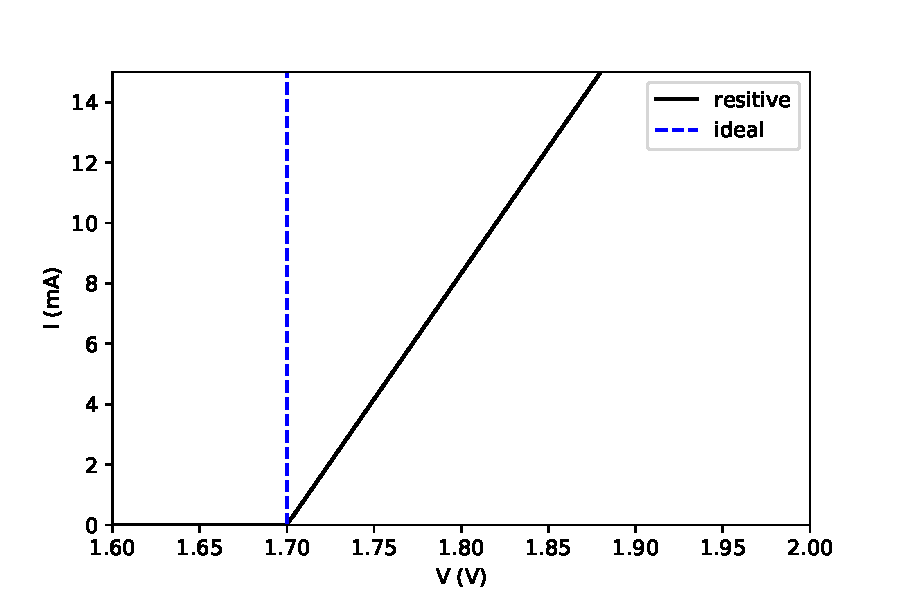
\includegraphics[height=0.3\textheight]{figs/labs/planck/model.pdf} \\
\end{center}
\caption{The LED model for $V_A=1.7~\rm V$ and $R_{\rm LED}=12~\Omega$}
\label{fig:ledmodel}
\end{figure}



\section{$V-I$ Curve from LED.}

\begin{figure}[htbp]
\begin{center}
\begin{circuitikz}[line width=1pt]
\draw (0,0) to[voltage source,bipoles/length=1.5cm,l=$V_1$] ++(0,4.0) to[short] ++(2.0,0) coordinate(C);
\draw (C) to[R, l_=$R_1$] ++(0,-2.0) coordinate(B) to[empty diode, l_=LED] ++(0,-2.0) coordinate(A) to[short] ++(-2.0,0.0);
\draw (A) to[short,*-] ++(1.5,0) to[short] ++(0,0.8) node[component]{V} to[short] ++(0,0.8) to[short,-*] ++(-1.5,0);
\draw (C) to[short,*-] ++(1.5,0) to[short] ++(0,-0.8) node[component]{V} to[short] ++(0,-0.8) to[short,-*] ++(-1.5,0);
\end{circuitikz} 
\end{center}
\caption{experimental setup.}
\label{fig:planck_setup}
\end{figure}

Construct the experimental setup shown in Fig.~\ref{fig:planck_setup}
using a $1~\rm k\Omega$ precision $1\%$ resistor for $R_1$, a green
LED (see Table~\ref{tbl:led}) , and using your bench-top DC supply to provide $V_1$, initially
set to $0~\rm V$.  Connect Mastech voltmeter across the resistor $R_1$ and
Triplett voltmeter across the LED.  When constructing your circuit,
make sure the LED can be easily removed and replaced.  Also keep in
mind that the longer lead is the positive terminal of the LED, i.e.,
the upper terminal of the LED as drawn in the
Fig.~\ref{fig:planck_setup}.  Set both voltmeters to the $20~\rm V$
setting.

Test your circuit first by turning up the voltage on your supply to
about $5~\rm V$ and checking that the LED lights up.  The voltmeter
across the resistor $R_1=1~\rm k\Omega$ is effectively measuring the
current in $mA$ as $1~{\rm V}/1~{\rm k\Omega} = 1~\rm mA$.  Do not
misunderstand this statement to mean you should set the multi-meter to
the current measurement: we measure the voltage, but from $Ohm's Law$
we know the current in resistor.  The voltmeter across the diode is
measuring the diode drop $V_{\rm D}$.

$I = 0.5,1.0,2.0,4.0,6.0,8.0,10.0,12.0~\rm mA$ are target values for your current. 
Take a series of measurements of $V_{R_1}$ and $V_D$ near target values of $I$
by adjusting the voltage provided by your DC supply until the current $I$, as derived from measured
voltage across $R_1$, is near the target value.  Remember
not to waste time fussing to make the measurement at exactly the
target value.  For instance, measuring at $I=2.16~\rm mA$ instead of
the target $I=2.0 ~\rm mA$ is perfectly acceptable.  
\begin{measurement} Record a sketch of your setup in the logbook. 
\end{measurement}
\begin{measurement} 
Record in your logbook the measured values of $V_{\rm R_1}$, the accuracy $\Delta V_{\rm R_1}$, $I$ derived from $V_{\rm R_1}$, uncertainty $\Delta I$, measured values of  $V_{\rm D}$ and the accuracy $\Delta V_{\rm D}$. In addition record the fractional uncertainty of $I$ and $V_{\rm D}$. See table~\ref{tbl:example} for example on how to log the data. See table~\ref{tbl:accuracy} for accuracy of the multimeters. You  can neglect uncertainty on $R_1$ value when calculating uncertainty of $I$.
\end{measurement}
 

\begin{table}
\begin{center}
\caption{Example of table to record data.
\label{tbl:example}
%Instructor data from a red LED not used
}
%\begin{tabular}{lll}
%target $I$ (mA) & $I$ (mA) & $V_{\rm D}$ (V) \\
%\hline
%0.5  &  0.44  & 1.62 \\
%1.0  &  0.95  & 1.66 \\
%2.0  &  1.99  & 1.71 \\
%4.0  &  4.15  & 1.77 \\
%6.0  &  6.05  & 1.81 \\
%8.0  &  8.09  & 1.85 \\
%10.0 &  10.04 & 1.88 \\
%12.0 &  12.02 & 1.91 \\ 
%\end{tabular}
\begin{tabular}{llllllllll}
target $I$ (mA) & $V_{\rm R_1}$ (V) & $\Delta V_{\rm R_1}$ & $I$ (mA) & $\Delta I$ & \% $I$ &$V_{\rm D}$ (V) & $\Delta V_{\rm D}$ (V) & \% $V_{\rm D}$ \\
\hline
0.5 & \dots &  \dots &  \dots & \dots  & \dots & \dots & \dots & \dots  \\
\end{tabular}
\end{center}
\end{table}

\begin{measurement} 
Repeat this measurement using a yellow LED (see Table~\ref{tbl:led}).
\end{measurement}

\begin{measurement} 
Repeat this measurement using a red LED (see Table~\ref{tbl:led}).
\end{measurement}


\begin{table}[htbp]
\begin{center}
\caption{LEDs used in this experiment.}
\label{tbl:led}
\begin{tabular}{llll}
color & part no. & $\lambda$ (nm) & max current \\
%blue  & WP710A10QBC & 460 & 30 mA \\
green & WP710A10GT & 565 & 25 mA \\  
yellow & TLHY4405 & 581-594 & 30 mA \\ 
red & TLHR4405 & 612-625 & 30 mA \\ 
\end{tabular}
\end{center}
\end{table}

\section{Analysis}

\begin{figure}[htbp]
\begin{center}
\begin{tabular}{cc}
\includegraphics[width=0.45\textwidth]{figs/labs/planck/fit_diode.pdf} &
\includegraphics[width=0.45\textwidth]{figs/labs/planck/fit_vi.pdf} \\
(a) & (b) \\
\end{tabular}
\end{center}
\caption{Example fit for red LED.  The (a) real diode response
  departs from the simple linear model for $I \leq 2~\rm mA$, so the
  (b) fit for the linear response is performed for $I > 2~\rm mA$.
  Note that $V_{\rm D}$ is taken as the $y$-axis for the purpose of fit,
  because the voltage uncertainties are the dominant uncertainty in
  the fit.  Notice also that the $0.02~\rm V$ uncertainty reported by
  the DMM specifications appears to be predominantly systematic.}
\label{fig:redfit}
\end{figure}

The example of the V-I response for a red diode is
plotted in Fig~\ref{fig:redfit}a.  Notice that at large values for the
current ($I > 2~\rm mA$) the V-I response is linear, indicating that it
is dominated by internal resistance of the diode.  As lower current
($I \leq 2~\rm mA$) the V-I response is exponential, as expected for a
real diode.  We will fit our simple linear model for the diode
response only in the region where this approximation is valid, for
$I>2~\rm mA$. 

As shown in Fig.~\ref{fig:redfit}b, perform a linear
fit only for the data with $I>2~\rm mA$.

%With the DMM set to the $20~\rm V$ scale, the uncertainty on your
%measured values for $V$ and $I$ is approximately $0.02~\rm V$ and
%$0.02~\rm mA$ respectively.  



\begin{measurement} 
Because the measured voltage range is
less than a volt, but the measured current range is around $10~\rm
mA$, it is the uncertainties on the voltage that dominate the
uncertainty on both the slope and intercept of the linear function in our fit range. Show this is true for your measurement by looking at the percent uncertainties of $I$ and $V_{\rm D}$ that you recorded in your logbook. Record your observation in the logbook.
\end{measurement}


We therefore choose to use $V$ as the $y$-axis and and $I$ as the
$x$-axis for the purposes of fitting, because the $\chi^2$ analysis of
the {\rm curve{\_}fit} function only considers uncertainties in the
$y$-axis.  There are straightforward ways to handle uncertainties in
both $x$ and $y$, but they add complexity which is best avoided if
possible.

\begin{plot} For red LED data, fit the $V$ versus $I$ data to a linear function, and
determine the best fit resistance and activation voltage, and the
uncertainties.  
%Assume the uncertainty on the measured voltages is $0.02~\rm V$ for each data point 
Use uncertainties on the measured voltages
and only consider $I > 2~\rm mA$ in
the fit.  Remember to set {\tt absolute(\_)sigma=True} in your fit so
that the fit uncertainties are based on the absolute uncertainties
without re-scaling. \end{plot}

\begin{plot} 
Repeat this analysis for yellow LED data.
\end{plot}

\begin{plot} 
Repeat this analysis for green LED data.
\end{plot}

\begin{figure}[htbp]
\begin{center}
\includegraphics[height=0.3\textheight]{figs/labs/planck/planck.pdf} \\
\end{center}
\caption{Example plot for determination of $hc$.}
\label{fig:planckfit}
\end{figure}

\begin{plot} 
Plot the best-fit $V_A$ of each diode versus $1/\lambda$, and
determine the slope ($hc/e$) and its uncertainty from a linear
fit.  The example plot is shown in Fig.~\ref{fig:planckfit}.
Recall that $1~\rm eV$ is the change in potential energy of one
electron passing through $1~\rm V$ of potential energy, allowing you
to conveniently convert the slope in $\rm V \mu m$ to $\rm eV \mu m$ for
comparison with the established value $hc = 1.240~\rm eV \mu m$.
\end{plot}
\begin{print}
Does your measured value of  $hc$ agree with the known value? Print how many  sigma values your  measured value lies with respect to the known value, as well as your brief comment on this.
\end{print}


\section{Systematic Uncertainties}

In addition to the statistical uncertainties reported by the fit,
their are a number of systematic uncertainties.  For this lab, we'll
consider one obvious source of systematic uncertainty, which arises
from our treatment of the real diode response as a simple linear
function.

To determine the size of this systematic uncertainty, we measure the
effect of this assumption on our measured valued.  One simple way to
estimate this effect is to remove the requirement $I>2~\rm mA$ from
our analysis.  The difference between the measured value for $hc$ as
determined with and without the cut on $I>2~\rm mA$ can be interpreted
as a systematic uncertainty due to our simplistic model.

\begin{print} Repeat your analysis without the requirement $I > 2~\rm mA$ and take
this as the overall systematic uncertainty on your measurement. Print your result in the following form 
\begin{displaymath}
 \textbf{hc}= \textit{your value here} \pm \textit{your value here} \,  ({\rm stat}) \pm\textit{ your value here} \, ({\rm syst})
\end{displaymath}
\end{print}

\noindent
This is a \textbf{sign-off point} for this lab. 














\chapter{Muon Lifetime}

\section{Introduction}

\begin{figure}[htbp]
\begin{center}
{\includegraphics[width=0.35\textwidth]{figs/labs/muon/cosmic_ray.jpg}}\\
\end{center}
\caption{\label{fig:cosmic}  Cosmic ray shower induced by a primary cosmic ray (typically protons) striking an atom in the upper atmosphere.}\end{figure}

The muon is a fundamental particle in the Standard Model of particle
physics.  It is essentially a heavier version of the electron.  Like
the electron, the muon has a corresponding anti-particle, the
anti-muon ($\mu^+$).  Muons are readily available for study because
they are produced as a result of showers that are induced by incident
cosmic rays that constantly bombard the earth.  Typical primary cosmic
rays are protons, and there collisions with nuclei in the upper
atmosphere produce mainly protons, neutrons, and pions.  The
subsequent decays of these particles produce electrons, neutrinos, and
the muons we will be studying.  The flux of muons at sea-level is
about 1 per ${\rm cm}^2$ per minute, and this population has a mean
kinetic energy of about $4~\rm GeV$.  Such muons are highly
penetrating: they pass quite readily through buildings.

The muon decays via the weak interaction, its most probable decays being:
\begin{eqnarray*}
\mu^- \to e^- + \bar{\nu}_e \nu_\mu,\\
\mu^+ \to e^+ + \bar{\nu}_\mu \nu_e.
\end{eqnarray*}
As fundamental particles, muons are indistinguishable from one
another, and therefore the decay rate for a population of $N$ muons
must be simply proportional to $N$:
\begin{displaymath}
\frac{dN}{dt} = -\frac{N}{\tau}
\end{displaymath}
The solution to this differential equation is:
\begin{displaymath}
N(t) = N(0) \exp(-t/\tau).
\end{displaymath}
In this lab, you will measure the lifetime of the muon, which has the value 
\begin{displaymath}
\tau_\mu = 2.1969811(22) \mu s
\end{displaymath}
in vacuum as reported by the Particle Data Group (PDG) with the
uncertainty in parenthesis.  Interactions with the scintillator
material in this experiment lead to a slightly different expectation
for the lifetime as discussed below.

Muons are produced at a typical height $15~\rm km$ above sea-level,
and so, in the earth frame, their transit time from the upper
atmosphere to our lab is therefore about $50~\rm \mu s$ or about 20
lifetimes.  The fact that we see an appreciable number of them at sea
level, given an upper limit on their production rate in the
atmosphere, is clear evidence for time dilation.

\section{Experimental Setup}

\begin{figure}[htbp]
\begin{center}
{\includegraphics[width=0.55\textwidth]{figs/labs/muon/setup.png}}\\
\end{center}
\caption{\label{fig:setup}  Experimental setup.}\end{figure}

The active component of the particle detector used in this experiment
is a polyvinyltoluene-based plastic scintillator in the shape of a
cylinder with a $15~\rm cm$ diameter and a $12.5~\rm cm$ height.  All
materials absorb energy due to the passage of ionizing radiation.
Scintillators are materials which re-emit a fraction of this energy as
visible light, typically in the blue to near UV range.  The light
yield is relatively low, so a sensitive photomultiplier tube is used
to amplify a modest number of photons into a large easily measurable
voltage.

\begin{figure}[htbp]
\begin{center}
{\includegraphics[width=0.65\textwidth]{figs/labs/muon/cosmics_raw.pdf}}\\
\end{center}
\caption{\label{fig:cosmics_raw}  Three days of cosmic ray data, plotted as the distribution in digitized time measurement (TDC counts).}
\end{figure}


Muons are therefore constantly passing through the scintillator,
depositing energy, and causing observable PMT pulses which are
recorded by the data acquisition system (DAQ).  Occasionally, however,
a relatively low-energy muon enters the scintillator and deposits all
of it's kinetic energy, coming to rest.  As an unstable particle, it
eventually decays into a highly-energetic electron and neutrinos.  The
electron deposits additional energy in the scintillator which is
observed as a second pulse.  The time interval between two consecutive
pulses is digitized using a time-to-digital (TDC) converter, which
converts analog time interval into a digital number.  In this case, we
use a 12-bit TDC, so the measured digital values are integers in the
range from 0 to $2^{12}-1 = 4095$.  To interpret these raw TDC counts
as a time value in microseconds, you will need to calibrate the TDC as
described below.

Three days of data has already been collected for you, and is plotted
in Fig.~\ref{fig:cosmics_raw} .  This data is available on the course
web site in the file {\tt cosmics.npy} available You load this data
using the numpy {\tt load} command, taking care to handle the
directory path correctly.  As can be seen from the plot, most of the
recorded events have the maximum possible value 4095.  This is how the
DAQ records a single pulse, with no secondary pulse in the timing
window of the TDC.  This is what happens most of the time.

The remaining events, with a measured time below the maximum value, are from events were two pulses were detected within the timing window of the TDC.  This time
interval, the decay time of the muons in this population, will have a
time-dependence given by:
\begin{displaymath}
-\frac{dN}{dt} = \frac{N(0)}{\tau} \exp(-t/\tau)
\end{displaymath}
which you will use to extract the muon life time.  This is possible because the muon decay rate ($\lambda$)
and it's lifetime $\tau$ are simply recipocrals:
\begin{displaymath}
\lambda \equiv \frac{-\frac{dN}{dT}}{N(t)} = \frac{1}{\tau}.
\end{displaymath}
This exponential decay feature is clearly visible in the raw data as the downward sloping line on the right side of this semilog plot.

There is an additional source of background for two pulse events, which arises from the possibility for two muons to arrive independently within the time window of the TDC.   Sine the arrival time of the two muons is independent, this contribution is flat in time, and is clearly visible in the raw data on the left-hand side, where the exponential contribution becomes small.

\section{Calibration}

\begin{figure}[htbp]
\begin{center}
{\includegraphics[width=0.65\textwidth]{figs/labs/muon/pulser_4_raw.pdf}}\\
\end{center}
\caption{\label{fig:pulser_raw}  Calibration run with pulses spaced $4~\mu s$ apart.}
\end{figure}

To interpret the output of the TDC (digital TDC counts as integers in
the range from 0 to 4095) as physical times in units of microseconds,
a calibration is needed.  We are using a good TDC which we can assume has a linear response, meaning that the time interval and TDC counts are related as:
\begin{displaymath}
TDC = a \cdot \Delta t  + b 
\end{displaymath}

To determine the calibration parameters $a$ and $b$ we use an LED
pulser feature built into the detector.  The LED pulser feature
flashes light into the PMT in a controlled manner, so that two pulses
a distance $\delta t$ in time apart are sent repeatedly to the TDC.
An example of 1000 pulser events with $\Delta t = 4 \mu s$ is shown in
Fig.~\ref{fig:pulser_raw}.  A total of four pulser runs of 1000 events
each with $\Delta t = 1,2,4,8$ have already been collected.  The data
from these four calibration runs available on the course website with
names like {\tt pulser{\_}4.npy} for the $\Delta t = 4~\rm \mu s$ run.

{\bf Plot 1:}  for each pulser run, compute the mean value of the recorded data and an uncertainty on this mean value.
Plot these mean values, and their uncertainties, versus $Delta t$.  Fit the linear response to obtain the parameters $a$ and $b$.  Plot the best fit linear function alongside the data.

\section{Muon Lifetime Analysis}

{\rm Plot 2: } With the calibration constants $a$ and $b$ convert the
TDC counts of the recorded comsics data and plot the distribution of
times.  You should omit all events with RAW TDC count of 4095, as
these are single pulse events.  Fit the distribution to an exponential
function plus a constant value for the flat (combinatoric) background.
Plot your fit function against the recorded data.

Report the statistical uncertainty on the fitted value for
the muon lifetime.  In addition, there are several systematic
uncertainties associated with the experiment.  The largest is the
effect of material interactions on the lifetime of the muon, which is
about $5\%$.  Other systematic effects are smaller, and can be
neglected.


%\section{Muon / Anti-Muon Ratio}

%Due to additional decay processes when captured by an atomic nucleus, the decay time of the negatively %charged muon in matter is lower than its free space value:
%\begin{eqnarray*}
%\tau_- &=& 2.043(3) \times 10^{-6} \mu s \\
%\tau_+ &=& 2.1969811(22) \times 10^{-6} \mu s
%\end{eqnarray*}
%where we have used the measured values in carbon, which should be close to value for our organic %scintillator.

%As discussed in class, you can determine the ratio $\rho$ of anti-muons to muons from the relation:
%\begin{displaymath}
%\rho = - \frac{\tau_+}{\tau_-} \cdot \frac{\tau_- - \tau}{\tau_+ - \tau}
%\end{displaymath}
%where $\tau$ is the measured valued of the muon lifetime.



\end{document}

% OTHER IDEAS:
% Fourier Transforms
% Monte Carlo techniques
% Speed of Light in Cable
% Measure e from shot noise
